% LaTeX 2e Document.
% 
% $Id: user_man.tex,v 1.12 2006/04/19 10:27:25 vdmtools Exp $
% 

%%%%%%%%%%%%%%%%%%%%%%%%%%%%%%%%%%%%%%%%
% PDF compatibility code. 
\makeatletter
\newif\ifpdflatex@
\ifx\pdftexversion\@undefined
\pdflatex@false
%\message{Not using pdf}
\else
\pdflatex@true
%\message{Using pdf}
\fi

\newcommand{\latexorpdf}[2]{
  \ifpdflatex@ #2
  \else #1
  \fi
}

\newcommand{\pformat}{a4paper}

\makeatother
%%%%%%%%%%%%%%%%%%%%%%%%%%%%%%%%%%%%%%%%

\latexorpdf{
\documentclass[\pformat,12pt]{article}
}{
\documentclass[\pformat,pdftex,12pt]{article}
}

\usepackage[dvipdfmx]{graphicx, color}
\usepackage[dvipdfmx,bookmarks=true,bookmarksnumbered=true,colorlinks,plainpages=true]{hyperref}
\usepackage{alltt}
\usepackage{makeidx}
\usepackage{ifthen}
\usepackage{verbatim}
\usepackage{cite}

\usepackage{toolbox}
\usepackage{vdmsl-2e}


\usepackage{ascmac}

\graphicspath{{figures/}}
\def\seename{$\Rightarrow$}


\makeindex

\def\vdmsl{{\small VDM-SL}}
\def\vdmpp{{\small VDM}++}
\newcommand{\vdmslpp}{VDM-SL}
\newcommand{\vdmslppEm}{VDM-SL}
\newcommand{\ToolboxName}{VDM-SL Toolbox}
\newcommand{\Toolbox}{Toolbox}
\newcommand{\toolbox}{Toolbox}
\newcommand{\vdmde}{vdmde}
\newcommand{\vdmgde}{vdmgde}
\newcommand{\vdmhome}{vdmhome}
%\newcommand{\vdmdeNineteen}{vdmde} % not in use
\newcommand{\vdmdeNineteenEl}{vdmde.el}
\newcommand{\VdmSlPp}{\VdmSl}
\newcommand{\vdmext}{vdm}
\newcommand{\vdmModView}{\guicmd{Module View}}

\newcommand{\vdmtoolsver}{v8.3.2}

\newcommand{\cg}{\vdmslpp\ to C++ Code Generator}

\newcommand{\subsubsubsection}[1]{\paragraph{#1}\mbox{}\\}

% The use of /VDMPP ifdef's have basicly been exchanged with the
% use of LaTeX ifthenelse's.  For this two LaTeX boolean value  and
% VDMpp have been defined  (Lowercase p's are used to avoid conflict with
% the VDMPP environment variable.  The typical use are:
%   \ifthenelse{\boolean{VDMsl}}{vdmsl-text}{vdmpp-text}
%   \ifthenelse{\boolean{VDMsl}}{vdmsl-text}{}
%   \ifthenelse{\boolean{VDMpp}}{vdmpp-text}{}
% The advantage of this as opposed to ifdef's is that within a general
% paragraph specific VDM-SL and VDM++ parts can be distinguished without
% problematic empty lines.
% 
% The values are initialised such that exactly one of the values is true
% and the other is false.  This should hopefully avoid strange behaviour
% due to possible preprocessing errors.  The default case is VDM-SL.
\newboolean{VDMsl}
%\setboolean{VDMsl}{true}
\newboolean{VDMpp}
%\setboolean{VDMpp}{false}
\newboolean{VDMrt}
\setboolean{VDMsl}{true}
\setboolean{VDMpp}{false}
\setboolean{VDMrt}{false}

% This macro can be used in `description' lists where
% the item given to `meti' is put on its own line,
% thereby giving proper (nicer) identation to the
% explanation.
\newcommand{\meti}[1]{\item[#1]\mbox{}\\}

\newcommand{\Index}[1]{#1\index{#1}}

\newcommand{\Lit}[1]{`#1\Quote}
\newcommand{\Rule}[2]{
  \begin{quote}\begin{tabbing}
    #1\ \ \= = \ \ \= #2  ; %    Adds production rule to index
  \end{tabbing}\end{quote}
  }
\newcommand{\SeqPt}[1]{\{\ #1\ \}}
\newcommand{\lfeed}{\\ \> \>}
\newcommand{\OptPt}[1]{[\ #1\ ]}
\newcommand{\dsepl}{\ $|$\ }
\newcommand{\dsep}{\\ \> $|$ \>}
\newcommand{\Lop}[1]{\Lit{\kw{#1}}}
\newcommand{\Sig}[1]{\Lit{{\tt #1}}}
\newcommand{\blankline}{\vspace{\baselineskip}}
\newcommand{\Brack}[1]{(\ #1\ )}
\newcommand{\nmk}{\footnotemark}
\newcommand{\ntext}[1]{\footnotetext{{\bf Note: } #1}}

%\usepackage[]{color}
\usepackage{longtable}
\usepackage{float}
\definecolor{covered}{rgb}{0,0,0}     %black
\definecolor{not_covered}{gray}{0.5}  %gray

%\restylefloat{figure}
\setcounter{topnumber}{3}
\def\topfraction{1.0}
\setcounter{bottomnumber}{3}
\def\bottomfraction{1.0}
\setcounter{totalnumber}{3}
\def\textfraction{.1}


\parindent0mm

\newlength{\keywwidth}

\newcommand{\xfigpicture}[4]{
\begin{figure}[hbt]
\setlength{\unitlength}{1mm}
\begin{center}
\mbox{
\begin{picture}(#1,#2)
\put(0,0){\special{psfile=#3 hscale=70 vscale=55}}
\end{picture} }
\end{center}
\caption{#4}
\end{figure}
}

%\newcommand{\qq}{\marginpar{\bf ???}}
\newcommand{\aaa}{\tt }
\newcommand{\cmd}{\tt }
\newcommand{\guicmd}[1]{{\sf #1}}
\newcommand{\keyw}[1]{{\sf #1}}
%\newcommand{\id}[1]{%
%  \settowidth{\keywwidth}{\tt #1}%
%  \protect\makebox[\keywwidth][l]{{\it #1}}}
%\nolinenumbering

\begin{document}
\vdmtoolsmanualscsk{VDMTools User Manual (\vdmslpp)}
       {\ifthenelse{\boolean{VDMrt}}{2.0 beta}{2.0}}

\section{Introduction} \label{introduction}

%This manual presents an introduction to the \vdmslpp\ \Toolbox.

\VDMTools\ is a set of tools that allows you to develop and analyse
precise models of computing systems. When used in the early stages of
system development, these models can serve as system specifications,
or as an aid in checking the consistency and completeness of user
requirements. The models are expressed either in the ISO VDM-SL
standard language \cite{ISOVDM96}\index{VDM Standard} or in the
object-oriented formal specification language VDM++
\cite{LangManPP-SCSK,Fitzgerald&05}. This manual describes the \vdmslpp\ Toolbox, which
provides a range of tools for automatic checking and validation of
models expressed in \vdmslpp\ 
prior to implementation. These range from traditional syntax and type
checking tools to a powerful interpreter that executes models on
request and performs automatic consistency checking during execution.
The execution facilities support the use of testing techniques in
early analysis and design and allow execution of entire test suites in
line with established software engineering practice.  Moreover, the
interpreter enables interactive debugging of models by setting
breakpoints, stepping through statements and expression evaluations,
inspecting the call stack, and checking the values of variables in
scope.

This document provides an introduction and reference manual to the
\vdmslpp\ Toolbox (called the \Toolbox\ in the remainder of the
document). The \vdmslpp\ language is described in the separate
language reference manual
\ifthenelse{\boolean{VDMsl}}{\cite{LangMan-SCSK}}{\cite{LangManPP-SCSK}}. In the
remainder of this manual we use the term {\em specification\/} to
refer to any model constructed in the language for whatever purpose.


\subsection*{VDM Input Formats}\index{Input!Formats}

The \Toolbox\ supports \vdmslpp\ specifications embedded in either
Microsoft Word or \LaTeX\ documents so that it is possible to analyse
specifications without having to extract them into a special file. We
recommend the use of either one of these two approaches as an
excellent way of combining the model of a system with its
documentation. Having just one version of the specification helps to
avoid inconsistencies arising between working and documented versions
of the specification. If you would rather not use Word or \LaTeX, you
can of course write specifications as clear text in plain ASCII files
using your preferred text editor.

The \Toolbox\ supports input documents in a range of different
languages and scripts\index{Input!Generic}. 
Appendix~\ref{sec:generic} explains how to 
configure the \Toolbox\ for different scripts. 

If you use Microsoft Word to write your \vdmslpp\ specifications, you
should save the documents containing specifications in {\em rich text
  format\/}~(RTF). The \Toolbox\ distribution contains example files in
this format. Throughout this manual, you will see examples using files
from the \Toolbox\ distribution. The names of such example files are
followed by the extension ``{\tt .rtf}'', indicating that they are in
rich text format. 

In this manual we will normally introduce features of the \Toolbox\ 
using Word and RTF.  If you use the \LaTeX\ text processing system to
write your specifications, then note that the \Toolbox\ expects input
containing \LaTeX\ commands mixed with VDM specifications using the
style and format described in Appendix~\ref{sec:latexANDvdm}. The
\Toolbox\ distribution also contains example files in this format,
indicated by the filename extension ``{\tt .\vdmext}'' rather than
``{\tt .rtf}''.  Thus, if an example refers to a file called {\tt
  sort.rtf}, you should instead use the file {\tt
  sort.\vdmext}. References to a directory structure are shown
throughout this manual in the form {\tt examples/sort.vdm} (i.e.\ with a
forward slash)   unless the reference is only relevant under Windows
in which case  it is shown as \verb+examples\sort.vdm+ (i.e.\ with a
backward slash).

If you prefer to write specifications as plain text ASCII files, 
note that the only way to incorporate explanatory text into your
specification is by means of the \vdmslpp\ comment syntax, described
in the Language Manual. Files prepared in this format are normally
given a ``{\tt .\vdmext}'' extension.


\subsection*{Using This Manual}

This manual is divided into three parts. Sections~\ref{sec:overview}
and~\ref{sec:guidedtour} provide an overview of the various tools in
the \Toolbox\ and a ``hands-on'' tutorial introduction to using the
\Toolbox\ via its graphical user interface.  Before working through
this part of the manual the \Toolbox\ should be installed and the
environment variables required should be set~(see
Appendix~\ref{sec:set_env}). The installation of the \Toolbox\ is
described in the document
\ifthenelse{\boolean{VDMsl}}{\cite{InstallMan-SCSK}}{\cite{InstallPPMan-SCSK}}.
As you work through Section~\ref{sec:guidedtour}, you will get to know
the various tools and control commands available to you.

The second part of the manual~(Section~\ref{sec:ref}) is a reference
guide covering all the features of the \Toolbox\ systematically. All three
available interfaces -- the command line interface, the Emacs interface
and the graphical user interface -- are described for each feature.

The third part of the manual consists of appendices on a range of
topics. 
%Appendix~\ref{ifadsupport} explains how to contact IFAD for support for the \Toolbox.
 Appendix~\ref{sec:vdmlinks} includes
pointers to information resources for VDM, including internet sites,
project descriptions, technical papers and books.
Appendix~\ref{sec:latexANDvdm} explains how you merge text and
specification in \LaTeX\ documents.

% \ifthenelse{\boolean{VDMsl}}{}{Appendix~\ref{sec:inheritex} presents a small
%   example used for illustration purposes in the reference part of this
%   manual.} 
Appendix~\ref{sec:set_env} describes which environment
variables and options can be set for the \Toolbox.
Appendix~\ref{getting-started} describes the Emacs interface.
Appendix~\ref{sec:testscript} presents a few test scripts used for
systematic testing of the sorting specification which is used as a
running example in this manual. \ifthenelse{\boolean{VDMsl}}{And}{} 
Appendix~\ref{sec:trouble} offers some possible solutions 
to common problems encountered when using the \Toolbox\ in conjunction
with Microsoft Word. \ifthenelse{\boolean{VDMsl}}{}{And 
Appendix~\ref{sec:priorityfile} describes the format for defining
priority files for use with the interpreter.} 


\newpage

\section{\protect\VDMTools\ Overview}\label{sec:overview}

A \vdmslpp\ specification is a document which aims to describe the
properties of a system in a precise way. The specification can be
distributed among several files in the input formats described in
Section~\ref{introduction}.  Figure~\ref{fig:toolbox} provides an
overview of the functionality of the \Toolbox\ and its additional
features. The various tools are described below:


\begin{figure}
\begin{center}
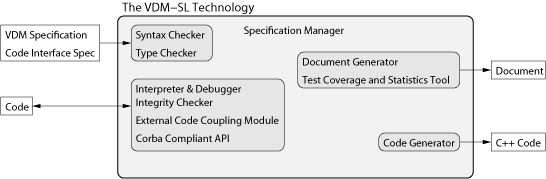
\includegraphics[width=10cm]{vdmtools_sl.png}
\caption{Overview of \protect\VDMTools}
\label{fig:toolbox}
\end{center}
\end{figure}

\begin{description}
  
\item[Specification Manager] The specification manager keeps track of
  the status of \ifthenelse{\boolean{VDMsl}}{modules}{classes} in the
  specification, which may be spread across several files.
 
\item[Syntax Checker] The syntax checker checks whether the syntax of
your \vdmslpp\ specification is correct with respect to the definition
of the \vdmslpp\ language. If the syntax is accepted it gives access
to the other tools in the \Toolbox.

\item[Type Checker]
  The type checker contains a powerful type inference mechanism which
  identifies mis-uses of values and operators and which can also show all
  places where run-time errors could occur.

\item[Interpreter and Debugger] The interpreter allows you
  to execute all the executable constructs in \vdmslpp. These range
  from simple value builders like set comprehension and sequence
  enumeration to more advanced constructs like exception handling,
  lambda expressions, loose expressions and pattern matching%
  \ifthenelse{\boolean{VDMpp}}{, or even multithreaded models}{}%
.  One of
  the benefits of executing specifications is that testing techniques
  can be used to assist in their validation. In the development
  process small or large parts of a specification can be executed to
  enhance the designer's knowledge of and confidence in the
  specification. Furthermore, an executable specification can form a
  running prototype.

  A source-level debugger is an essential aid when working
  with executable specifications. The \vdmslpp\ debugger supports the
  functionality found in debuggers for ordinary programming languages,
  including setting breakpoints, stepping, inspection of variables
  defined in the scope, and inspection of the call stack. 

\item[Integrity Examiner] The integrity examiner extends the static
  checking capabilities of the \vdmslpp\ Toolbox by scanning through
  specifications checking for potential sources of internal
  inconsistencies or integrity violations. The checks include the
  violation of data type invariants, preconditions,  postconditions,
  sequence bounds and map domains. Each \emph{integrity property} is 
  presented as a \vdmslpp\ expression which should evaluate to true --
  if it instead evaluates to false this indicates that there is a
  potential problem with the corresponding part of the specification. 

\item[Test Facility] The test facility allows you to exercise your
  specification using a predefined set of tests called a {\em test
    suite\/}. Test coverage information can be automatically recorded
  during execution of a test suite and presented back to the
  specifier, indicating which parts of the specification are most
  frequently evaluated and which parts have not been covered at all.
  The test coverage information is displayed directly in the source
  file which can be a Microsoft Word or \LaTeX\ document depending
  upon the input format used.

\item[Automatic Code Generator] The \Toolbox\ supports automatic
  generation of \ifthenelse{\boolean{VDMsl}}{C++}{C++ and Java} code
  from \vdmslpp\ specifications, helping to achieve
  consistency between specification and implementation. The code
  generator produces fully executable code for 95\%\ of all \vdmslpp\
  constructs, and there are facilities for including user-defined code
  for non-executable parts of the specification.  Once a specification
  has been tested, the code generator can be applied to obtain a rapid
  implementation automatically. The use of the C++ Code Generator is
  described in the document
  \ifthenelse{\boolean{VDMsl}}{\cite{CGMan-SCSK}}{\cite{CGManPP-SCSK}}% 
.

\item[Dynamic Link Facility] feature of the
  \Toolbox\ makes it possible to integrate external code into the
  execution of a specification.  This can be used to integrate a
  formal model with components developed in a traditional way and
  provide graphical front-ends for a model.  

\item[Corba Compliant API] The \Toolbox\ provides a Corba compliant
  Application Programmer Interface~(API) which allows other programs
  to access a running \Toolbox. This enables external control of the
  the \Toolbox\ components such as the type checker, interpreter and
  debugger. The API allows any code such as a graphical front-end or
  existing legacy code to control the \Toolbox.



\end{description}

\newpage

\section{A Guided Tour of the \protect\VDMTools} \label{guistart}
\label{sec:guidedtour}

This section provides a ``guided tour'' of the \Toolbox.  If you are
new to the principles of system modelling in VDM, we recommend that
you should first read either ``{\it Modelling Systems: Practical Tools and Techniques in
Software Development}''~\cite{Fitzgerald&98b}, by John Fitzgerald and
Peter Gorm Larsen or ``{\it Validated Designs for Object--oriented
Systems}''~\cite{Fitzgerald&05}. These are both tutorial books which 
includes many
examples built around VDM specifications which can be explored using
the \Toolbox. \cite{Fitzgerald&98b} is using the ISO standard VDM-SL
notation whereas \cite{Fitzgerald&05} is using the object-oriented
extension called \vdmpp. 
If you do have some knowledge about these general concepts,
\ifthenelse{\boolean{VDMsl}}{but are unfamiliar with the standard
  notation}{but are unfamiliar with the object-oriented extensions in
  \vdmslpp}, we recommend that you review the \vdmslpp\ language
reference manual ``{\it The  \vdmslpp\ Specification Language}''
\ifthenelse{\boolean{VDMsl}}{\cite{LangMan-SCSK}}{\cite{LangManPP-SCSK}}.


\subsection{Creating Input to \protect\VDMTools}\index{Input!Creating}

In order to use the \Toolbox\ it is necessary to produce a \vdmslpp\ 
specification. In this section we illustrate how to do that using
Microsoft Word in the rich text format (RTF) on a simple sorting
example. If you alternatively prefer using \vdmslpp\ combined with
\LaTeX\ you should consult Appendix~\ref{sec:latexANDvdm}\footnote{It
  is also possible to use plain ASCII \vdmslpp.}. In the remainder of
this section we assume some basic familiarity with Microsoft Word.

Start Microsoft Word by selecting it from the programs entry in the
Windows setup under Windows. Open the
\ifthenelse{\boolean{VDMsl}}{{\tt \vdmhome/examples/sort/sort.rtf}
  file}{{\tt \vdmhome/examples/sort/MergeSort.rtf} file} from the
\Toolbox\ distribution. Reading through this file, you will see that
the document is a mixture of explanatory text and a formal model in
\vdmslpp. All the formal parts are written in the style \texttt{VDM}.
You may not change the formatting of the text in the VDM style
directly in the source text. The pretty-printer will put VDM keywords
in the boldface font anyway. If you wish, you can modify the
appearance of this style, so long as the style's name is not changed:
the \Toolbox\ will only analyse those parts of the document written in
the \texttt{VDM} style.

A definition of the styles which are used by the \Toolbox\ inside
Microsoft Word can be found in the {\tt VDM.dot} file \index{VDM.dot file} 
from the \Toolbox\ distribution. This file can be copied to your template
directory (\verb+C:\Program Files\Microsoft Office\Templates+ normally)
so that these style definitions will be included if you
select this template when a new document is started (there are also
various ways in which the definitions can be copied into the template
file you normally use).

Now look at the end of the \ifthenelse{\boolean{VDMsl}}{{\tt sort.rtf} file}%
{{\tt MergeSort.rtf}} document.
You will see that there is an empty line typeset in the style \texttt{VDM\_TC\_TABLE}.
We will come back to the usage of this when we discuss how to record and display test coverage
information. The styles \texttt{VDM\_COV} and \texttt{VDM\_NCOV} are
also used in connection with test coverage information. We will also
come back to these styles later.

If you wish to gain more experience with using Microsoft Word for
producing your input to the \Toolbox\ we recommend that you try to
read in some of the other examples from the \Toolbox\ distribution
after completing this guided tour.


\subsection{Starting the \vdmslpp\ Graphical User Interface}\index{Graphical User Interface!Starting} 

The \Toolbox\ is normally used via its graphical user interface. Before
starting this interface, VDM source files should be copied into a
working directory. The \Toolbox\ distribution contains a specification
of different sorting algorithms, a presentation of which can be found
in the technical report
\ifthenelse{\boolean{VDMsl}}{\cite{SortEx-SCSK}}{\cite{SortExpp-SCSK}}.  During
this guided tour we will use this sorting specification as our running
example, so copy the directory {\tt \vdmhome/examples/sort} from the
\Toolbox\ distribution and {\tt cd} to it.  This will enable you to
try the tools in the \Toolbox\ directly on your computer while you are
following the tour.

The \Toolbox\ is started by selecting it from the ``Program Files''
entry in the Windows start menu or with the command {\tt \vdmgde}
\index{vdmgde command} on Unix platforms. The \Toolbox\ 
will start up as shown in Figure~\ref{fig:startgui}. This window is
called the {\em main window\/} of the \Toolbox.


\begin{figure}[tbh]
\begin{center}
\ifthenelse{\boolean{VDMsl}}{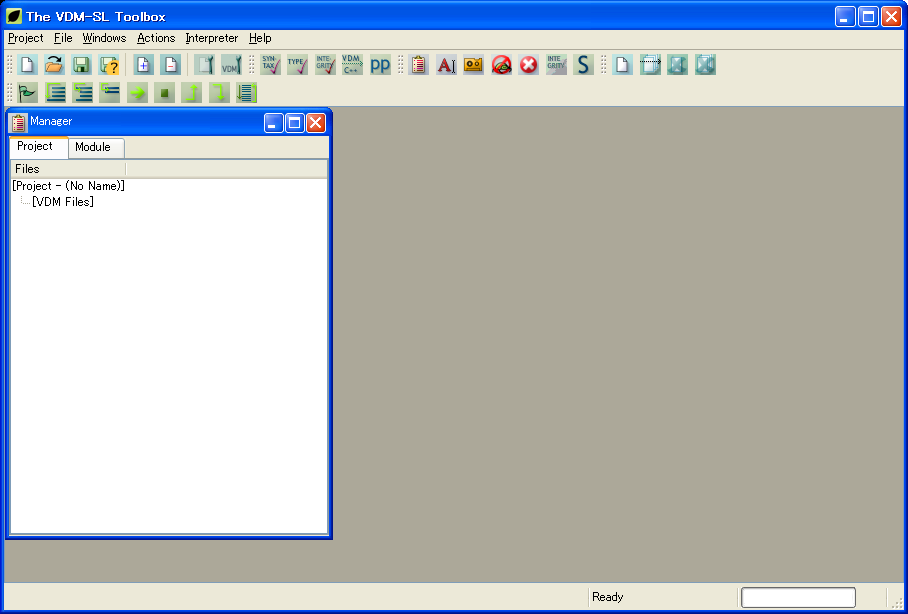
\includegraphics[width=11cm]{startgui-slENG.png}}{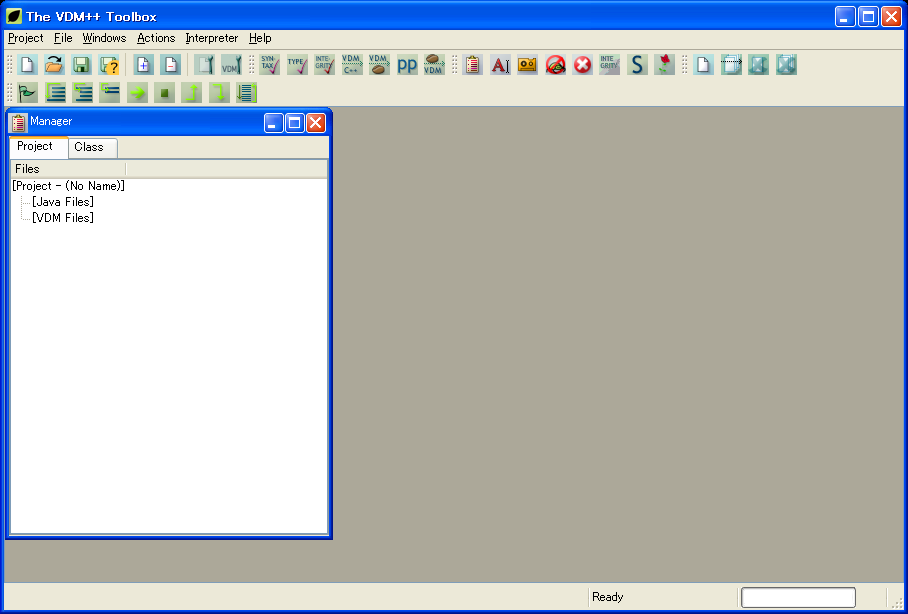
\includegraphics[width=11cm]{startgui-ppENG.png}}
\caption{Graphical User Interface Startup}
\label{fig:startgui}
\end{center}
\end{figure}

\subsection{On-Line Help}\index{Help}
 
% %%%%% The next paragraphs should be reinserted when help window is
% %%%%% implemented -- RM
%
% At any time when you are using the \Toolbox\ you can press the ``{\tt
%   F1}'' button and a help window~(as shown in
% Figure~\ref{fig:guihelp}) will appear with
% on-line help for the 
% graphical user interface. The part of the help text that is shown at
% the top of the help window is related to the particular part of the
% \Toolbox\ window in which the cursor is placed. The help text is
% organised in a hypertext format so it is possible to follow links from
% one part of the help text to another.

% \begin{figure}[tbh]
% \begin{center}
% #ifdef 
% \resizebox{\textwidth}{!}{\includegraphics{guihelp-sl}}
% #endif 
% #ifdef VDMPP
% \resizebox{\textwidth}{!}{\includegraphics{guihelp-pp}}
% #endif VDMPP
% \caption{The Help Window\label{fig:guihelp}}
% \end{center}
% \end{figure}

% The help window can also be accessed by pressing the  
% \raisebox{-0.8mm}{
\includegraphics[width=0.03\textwidth]{help}}
% button on the \guicmd{Help} toolbar or by selecting the corresponding
% item from the \guicmd{Help} menu. 

On-line help for the \Toolbox\ and the interface in general can %also
be accessed through the \guicmd{Help} toolbar or
the \guicmd{Help} menu. Currently only the following
very limited help is available:


\begin{description}
 \item[\guicmd{About} (\hspace{-1.8mm}
\raisebox{-0.8mm}{
\includegraphics[width=0.03\textwidth]{help.png}}):]
  Displays the version number of the \Toolbox.
 \item[\guicmd{aboutqt}  (\hspace{-1.8mm}
\raisebox{-0.8mm}{
\includegraphics[width=0.03\textwidth]{qt.png}}):]
  Displays information about and a reference to Qt, the multiplatform
  C++ GUI toolkit which the \Toolbox\ interface uses.
% \item[\guicmd{What's This?} (\hspace{-1.8mm}
%\raisebox{-0.8mm}{
\includegraphics[width=0.03\textwidth]{whatsthis}}):]  
%  Select this item then click the left mouse button over some part of
%  the \Toolbox\ to get a brief description of it. (Currently only
%  partly implemented.) \\
\end{description}

\subsection{Menus, Toolbars and Subwindows}

The top of the main window consists of a menu line with six pull-down menus:

\begin{description}
\item[\guicmd{Project}:] A project consists of a
  collection of file  
  names that together form a \vdmslpp\ specification. Under this menu
  heading it is possible to open and save projects, to configure (add
  files to and remove files from) projects, and to create new
  projects. This is also the place from which to exit the \Toolbox\
  and to set options for the various tools in the \Toolbox, for
  example to govern the level of type checking.

\item[\guicmd{File}:] Here you can invoke a file editor for making
  corrections to your specification and also remove displays of source
  files generated by the \Toolbox\ when it reports errors.

\item[\guicmd{Windows}:] Controls to determine which windows are
  displayed in the bottom pane of the main window. Each menu item
  toggles opening/closing of a particular window.

\item[\guicmd{Actions}:] This offers the various
  actions that can be applied to a specification: syntax and type
  checking, generation of integrity properties, code generation, 
and pretty printing.

\item[\guicmd{Interpreter}:] This offers
  functions for controlling the interpreter (see Section~\ref{interpreter}).
\end{description}

%  Below this menu line are six\footnote{When the \Toolbox\ is started,
%  only the three which correspond to the first, third and fourth menus are
%  displayed open; the other three are displayed in iconised form above
%  them.} toolbars comprising buttons which offer the same
%  actions\footnote{Except that the function for exiting from the toolbox
%  is only available on the \guicmd{Project} menu.}.
  Below this menu line are six toolbars comprising buttons which offer the same
  actions\footnote{Except that the function for exiting from the toolbox
  is only available on the \guicmd{Project} menu.}.
  
  Finally, the lower pane of the main window is used to display various
  subwindows which either present information about the status of the
  current project or offer interfaces to tools within the \Toolbox. The
  available windows are as follows:

\begin{description}
\item[\guicmd{Manager}]\index{Manager} Displays the current status of
  the current project. It consists of two parts:

  \begin{description}
  \item[\guicmd{Project View}]\index{Project View} This shows a tree
  representation of the contents of the project comprising the files in the project and
  (only after successfully syntax checking the file) the
  \ifthenelse{\boolean{VDMsl}}{modules}{classes} declared in each file.
  \ifthenelse{\boolean{VDMsl}}{
     \item[\guicmd{Module View}]\index{Module View} This displays the
       status of each of the individual \vdmslpp\ modules in the project.
  }{
     \item[\guicmd{Class View}]\index{Class View} This offers both a
  \guicmd{VDM View} 
       and a \guicmd{Java View}, which display the status of each of
       the individual \vdmslpp\ classes or Java files in the project
       respectively.} 
  \end{description}

\item[\guicmd{Source Window}]\index{Source Window}  Displays the part
  of the source specification in which the error currently selected in
  the \guicmd{Error List} was discovered.

\item[\guicmd{Log Window}]\index{Log Window} Displays messages from the \Toolbox.
% \item[\guicmd{References}] Displays the dependencies between classes,
%   that is the classes which use the selected class and the classes
%   which the selected class uses~(a class {\em uses\/} another class if it
%   has references to objects of that class, for example through its
%   instance variables or operation calls). 
\item[\guicmd{Interpreter Window}]\index{Interpreter Window} The
interface to the interpreter. 

\item[\guicmd{Error List}]\index{Error List} Reports errors found by the \Toolbox.
\item[\guicmd{Integrity Properties Window}] Displays the integrity properties
  that have been generated for the specification.
\end{description}

When the \Toolbox\ is started, only the \guicmd{Manager} is open.

\subsection{Configuring your Project}

First you need to configure the \Toolbox\ by indicating which 
files (in your desired input format) are to be analysed. For this
purpose you can select the action \guicmd{Add File to Project} on the
\guicmd{Project} menu or simply press the 
\raisebox{-0.4mm}{
\includegraphics[width=0.03\textwidth]{plus.png}}  
(\guicmd{Add Files}) button on the (\guicmd{Project Operations})
toolbar\footnote{In the remainder of this guided tour we concentrate
  on interactions via the toolbar buttons. You can of course always
  use the equivalent menu item if you prefer.}. The dialog box shown
in Figure~\ref{fig:addFiles} will then appear\index{Project!Adding files}.

\begin{figure}[tbh]
\begin{center}
\ifthenelse{\boolean{VDMsl}}{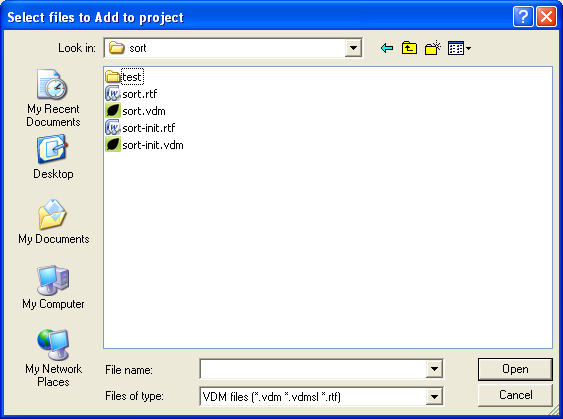
\includegraphics[width=11cm]{addFiles-slENG.png}}{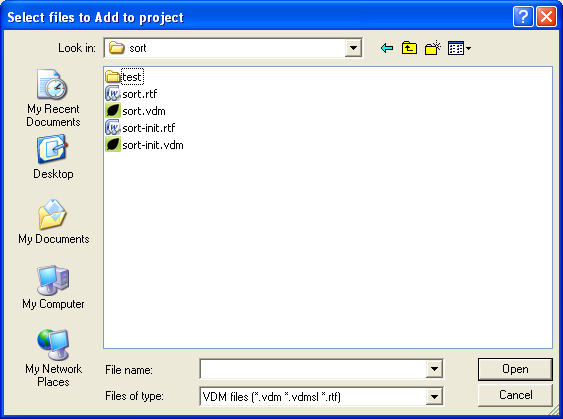
\includegraphics[width=11cm]{addFiles-slENG.png}}
\caption{Adding Files to a Project}
\label{fig:addFiles}
\end{center}
\end{figure}

\ifthenelse{\boolean{VDMsl}}{%
Here you double click on the {\tt sort-init.rtf} file (or select the
file and add it to the project by 
pressing the ``\guicmd{Add to project}'' button).  This file will then
be included in the project. You can mark more than one file at a time
by holding down the {\cmd Ctrl} key and clicking the left-hand
mouse button on each of the files in turn, and you can mark a list of
files by selecting the first and last files in the list (in either
order), holding down the {\cmd Shift} key while making the second
selection.  Note that {\tt sort-init.rtf} contains a number of
errors for illustration purposes in this guided tour.
}
{%
Mark the six {\tt .rtf} 
files (minus the {\tt MergeSort.rtf} file) by holding down the {\cmd
  Ctrl} key and clicking the left-hand mouse button on each of the
files in turn, then press the ``Open'' button.  These files will then
be included in the project. You can also add a single file to a
project by double clicking the left-hand mouse button on it (but note
that this also closes the dialog box so it is not an efficient way
of adding a number of files), and you can also mark a list of files at
the same time by selecting the first and last files in the list (in
either order), holding down the {\cmd Shift} key while making the second
selection. Note that {\tt MergeSort-init.rtf} contains a number of
errors for illustration purposes in this guided tour.
}

The \ifthenelse{\boolean{VDMsl}}{{\tt sort-init.rtf} file}{six {\tt .rtf} files}
  will now appear in the \guicmd{Project View}
  of the \guicmd{Manager} in the main \Toolbox\ window as
  shown in Figure~\ref{fig:addedfiles}.

\begin{figure}[tbh]
\begin{center}
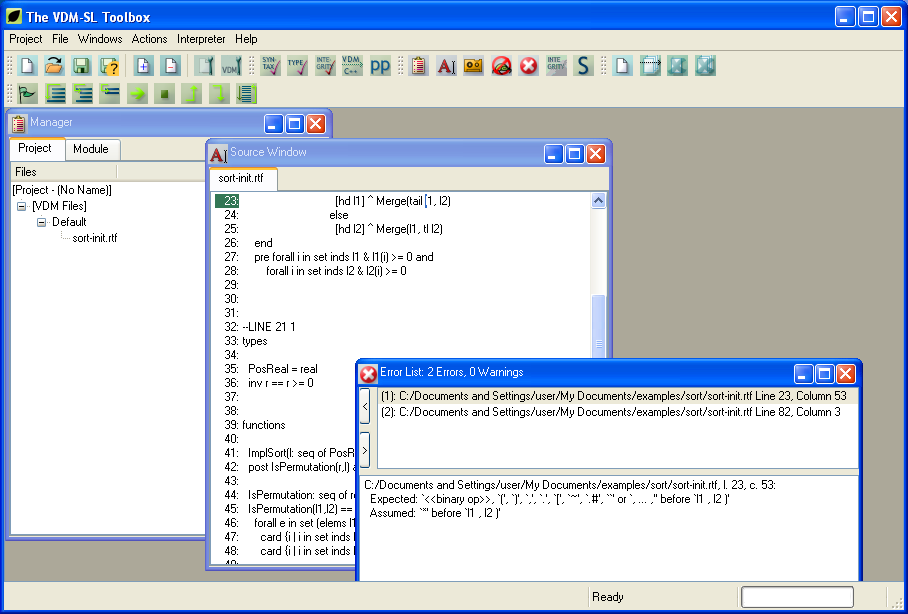
\includegraphics[width=11cm]{addedFiles-slENG.png}
\caption{Main Window After Addition of Files}
\label{fig:addedfiles}
\end{center}
\end{figure}


\subsection{Syntax Checking your VDM Specification}\index{SyntaxChecking}

Having configured your project you now need to check whether all the
\ifthenelse{\boolean{VDMsl}}{modules}{classes} obey the syntax rules
of \vdmslpp.  The syntax checker checks whether the syntax of your
specification is correct. Note that when you change a source file you
must syntax check it again before the other tools will be aware of the
changes you have made.


\subsubsection{Parsing the specification}

Select the files for syntax checking by
\ifthenelse{\boolean{VDMsl}}{clicking on the {\tt sort-init.rtf}
file}{marking the six {\tt .rtf} files} in the \guicmd{Project View}
of the \guicmd{Manager}, then press the 
\raisebox{-0.7mm}{
\includegraphics[width=0.03\textwidth]{syntaxcheck.png}}  
(\guicmd{Syntax Check}) button on the (\guicmd{Actions})
toolbar to invoke the syntax checker. (Selecting the containing level
 ``Default'' folder and applying the syntax check operation to that
 has the same effect -- this applies the operation to each of the
 files in the folder.) Notice that at this point the
\guicmd{Log Window} opens automatically (if it is not already open)
and displays the message 
\ifthenelse{\boolean{VDMsl}}{``{\tt Parsing "sort-init.rtf"
    ...}''}{``{\tt Parsing "..../DoSort.rtf" ...}'' etc.}.
(More than one file can be selected and
  in that case all of them are syntax checked.) If syntax
  errors\index{Syntax
  Errors} are discovered the \guicmd{Error List}\index{Error List} is
also au\-to\-matically invoked and the \guicmd{Source Window} is
automatically opened. Our sorting example contains two
deliberate syntax errors by way of illustration.


% \subsubsection{Traversing errors}
\subsubsection{Correcting syntax errors}\index{Syntax Errors!Correcting}

The \guicmd{Error List} is shown in Figure~\ref{fig:error}. Its top
pane shows a list of the places (file name, line number, column
number) at which errors and warnings arose, while the bottom
displays a more detailed explanation of the currently selected
error. Initially, the first error in the list is selected
automatically.


\begin{figure}[tbh]
\begin{center}
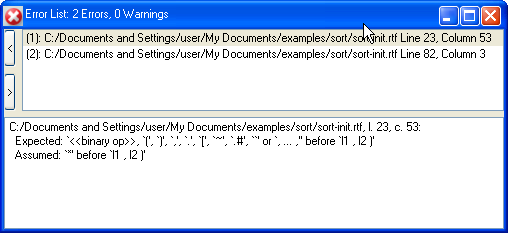
\includegraphics[width=\textwidth]{errorList-slENG.png}
\caption{The Error List}
\label{fig:error}
\end{center}
\end{figure}

The \guicmd{Source Window} displays the part of the source
specification in which the currently selected error was discovered,
the actual position being marked by the window's cursor. For the first
syntax error, the \guicmd{Source Window} appears as shown in
Figure~\ref{fig:source1}.

\begin{figure}[tbh]
\begin{center}
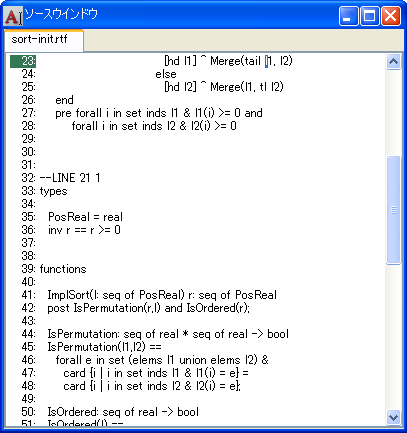
\includegraphics[width=9cm]{sourceWindow-sl.png}
\caption{The Source Window for the First Error}
\label{fig:source1}
\end{center}
\end{figure}

\newpage

The first error message is as follows:
\begin{verbatim}
C:/Documents and Settings/user/My Documents/examples/sort/sort-
    init.rtf, l. 23, c. 53:
  Expected: `<<binary op>>, `(', `)', `,', `.', `[', `~',
    `.#', ``' or `, ... ,'' before `l1 , l2 )'
  Assumed: `*' before `l1 , l2 )'
\end{verbatim}


Messages of this form indicate the text which was expected but not
found at the error point. The syntax checker reports the error and
makes an assumption about what should have been at the error point in
order to allow it to recover and carry on with the syntax check.

In our example, the error message tells us that a multiplication symbol
`{\tt*}' was assumed between `{\tt tail}' and `{\tt l1}' in order to
recover from the syntax error (the `{\tt tail}' symbol was read as the
name of an identifier). However, this assumption is incorrect and  you
can see from the  description of the \vdmslpp\ syntax in the Language
Manual~\cite{LangMan-SCSK} that the error is in fact that the `{\tt tl}'
operation which returns the tail of a sequence has been wrongly
written as `{\tt tail}'. The error can therefore be fixed by using the
file editor to rewrite `{\tt tail}' as `{\tt tl}'.

(Note that the source file is not changed by the syntax checker when
it ``assumes'' something: corrections to the source text should be
done manually by the user.)

You can correct the syntax errors by invoking your preferred editor
(see Appendix~\ref{sec:set_env}) directly from the \Toolbox\
interface. Select the file \ifthenelse{\boolean{VDMsl}}{{\tt
  sort-init.rtf}}{{\tt MergeSort-init.rtf}} in the main window and 
press the \guicmd{External Editor}\index{External Editor} button (%
\raisebox{-0.8mm}{
\includegraphics[width=0.03\textwidth]{externaleditor.png}}) 
on the (\guicmd{File Operations}) toolbar. Note that if more than
one file is selected when you invoke the \guicmd{External Editor} in
this way you actually get one \guicmd{External Editor} for each of the
selected files.

You can get to the next reported error by pressing the {\fbox{\tt >}}
button which appears to the left of the list of errors or by selecting the
error notifier directly in the top pane of the \guicmd{Error
  List}. Here the explanation is: 

\begin{verbatim}
C:/Documents and Settings/user/My Documents/examples/sort/sort-
    init.rtf, l. 82, c. 3:
  Expected: `<<binary op>>, `(', `.', `;', `operations', `state',
    `traces', `functions', `mease', `.#', `post', `pre',
    `types' or `values'' before `InsertSorted : PosReal *'
  Assumed: `;' before `InsertSorted : PosReal *'
\end{verbatim}

This tells us that there is a syntax error before `{\tt InsertSorted :
  PosReal *}' and that a preceding semicolon `{\tt ;}' was assumed in
  order to recover from the syntax error. In this case the assumption
  is in fact correct -- you can see from the  description of the
\vdmslpp\ syntax in \cite{UMLMan-SCSK} that two function definitions must
  be separated by the delimiter \Lit{;}. The error can therefore be
  fixed by returning to the file editor and adding the character
  \Lit{;} to the end of the definition of the function {\aaa DoSort}.



When you have corrected the syntax errors and saved the file, you must
re-run the syntax checker\index{Syntax Checking} to check your
corrections were right. This time the file should be syntactically
correct, and if you switch to the \vdmModView\ in the 
\ifthenelse{\boolean{VDMsl}}{}{(\guicmd{Class View} of the)} 
\guicmd{Manager} you will see 
that the status\index{Status Information} of 
\ifthenelse{\boolean{VDMsl}}{the module representing our specification
  (called {\tt DefaultMod} because no module structuring has
  been used in this small example)}{each of the six classes ({\aaa
    DoSort, ExplSort, ImplSort, MergeSort, Sorter, SortMachine}) in
  our specification} is now marked with the symbol 
\raisebox{-0.7mm}{
\includegraphics[width=0.03\textwidth]{syntaxcheckdone.png}}
in the syntax column indicating that it is syntactically
  correct. (See Figure~\ref{fig:vdmModView}.) Note that the blanks in the
other columns mean that no attempt has yet been made to type check,
code generate or pretty print  the specification.

\begin{figure}[tbh]
\begin{center}
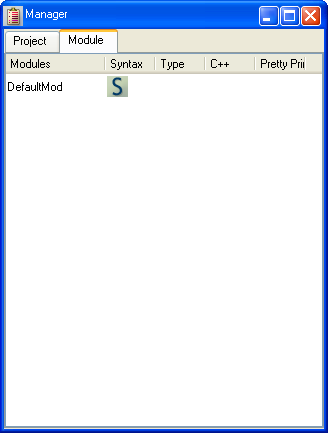
\includegraphics[width=9cm]{moduleViewENG.png}
\caption{The Module View}
\label{fig:vdmModView}
\end{center}
\end{figure}

Now that the syntax checking has been completed successfully, the
files can be selected for further processing directly in the \vdmModView.

\subsection{Type Checking your VDM Specification}
\index{Type Checking}\label{sec:gde-tc}

Once a specification has passed the syntax check, the type checker
can be applied. This is invoked by pressing the 
\raisebox{-1.0mm}{
\includegraphics[width=0.03\textwidth]{typecheck.png}}  
(\guicmd{Type Check}) button on the (\guicmd{Actions}) toolbar.

Select \ifthenelse{\boolean{VDMsl}}{the module {\tt DefaultMod}}{all
  six classes} in the \vdmModView\ and run the type 
checker. After type checking, the \Toolbox\ updates the status 
  information\index{Status Information} in this view to indicate,
using the symbols 
\raisebox{-1.0mm}{
\includegraphics[width=0.03\textwidth]{typecheckdone.png}}
and
\raisebox{-1.0mm}{
\includegraphics[width=0.03\textwidth]{typecheckerror.png}}
(this is the first symbol
\raisebox{-1.0mm}{
\includegraphics[width=0.03\textwidth]{typecheckdone.png}}
with a red line through it) 
respectively, whether the type check succeeded or failed for each
\ifthenelse{\boolean{VDMsl}}{module}{class}.

In this example it in fact failed \ifthenelse{\boolean{VDMsl}}{because
the sort specification}{for the {\tt MergeSort} class, which}
generated four type errors and one warning. The errors\footnote{The
  format of type errors is described in more detail in the reference
  part of this manual. See Section~\ref{type check}.} are displayed in
the \guicmd{Error List} as before.

The first error, which is shown in Figure~\ref{fig:type_error1},
is that the function {\tt Merge} is actually called with two sequences of
{\tt real} numbers (see the corresponding \guicmd{Source Window} shown in
Figure~\ref{fig:source-type}) whereas the types of the expected
parameters (as given in the signature for 
{\tt Merge}) are a sequence of {\tt int}~(integers) and a sequence of
{\tt bool}~(Boolean values). As {\tt int} is a subtype of {\tt real}
the first actual parameter could be type correct if all
the numbers in the sequences actually are integers. However, the
second parameter, which is supposed to be a sequence of {\tt bool},
causes the problem.  This error is corrected by changing {\tt bool} to
{\tt int} in the signature for the {\tt Merge} function.


\begin{figure}[tbh]
\begin{center}
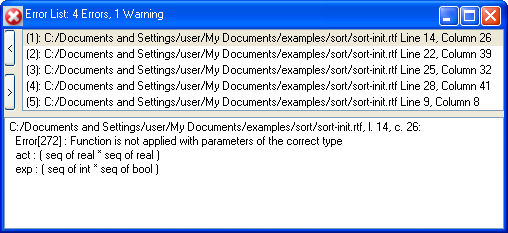
\includegraphics[width=11cm]{typeError1-slENG.png}
\caption{First error reported when type checking}
\label{fig:type_error1}
\end{center}
\end{figure}

\begin{figure}[tbh]
\begin{center}
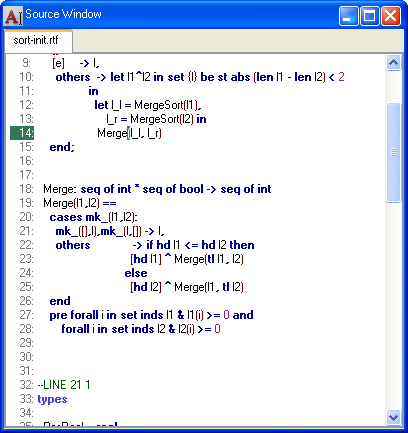
\includegraphics[width=9cm]{sourceWindow-type-slENG.png}
\caption{The Source Window for the Type Errors}
\label{fig:source-type}
\end{center}
\end{figure}

The second error, which is shown in Figure~\ref{fig:type_error2},
tells us that we tried to apply the \Sig{<=} operator with a
right-hand argument (Rhs) which does not belong to a numeric
type. More specifically, the actual argument (denoted by the keyword
{\sf act:} in the error message) is of type {\tt bool} while the 
expected argument (denoted by the keyword {\sf exp:}) is a real number
({\tt real} is the most general numeric type). Information like this
can be valuable when trying to determine the cause of an error.


\begin{figure}[tbh]
\begin{center}
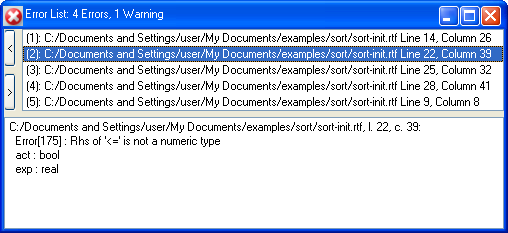
\includegraphics[width=11cm]{typeError2-slENG.png}
\caption{Second error reported when type checking}
\label{fig:type_error2}
\end{center}
\end{figure}

\ifthenelse{\boolean{VDMsl}}{This error, as well as the third error
which is similar except that it involves the left-hand argument (Lhs) of
the \Sig{<=} operator, is in fact also caused by having written {\tt
  seq of bool} instead of {\tt seq of int} in the signature of the
{\tt Merge} function. Thus, both of these errors are just 
follow-on errors from the first one. So just correct the first
error}{This mistake is in fact caused by the {\tt seq of bool} in the
signature of the {\tt Merge} function, which should be {\tt seq of
  int}. The same mistake also caused the third error, which is similar
to the second, and this disappears when the second error is
removed. So just correct the first two errors} and syntax and type
check the specification again.

Notice how the status information in the main window is updated
during this process. First, when the source file is edited the symbol 
\raisebox{-0.7mm}{
\includegraphics[width=0.03\textwidth]{syntaxcheckdone.png}}  
which indicated in the \vdmModView\ that the file was
syntactically correct is replaced by the symbol 
\raisebox{-0.7mm}{
\includegraphics[width=0.03\textwidth]{syntaxcheckmodified.png}}
indicating that there is an inconsistency between the version
currently in the \Toolbox\ and the version on the file system. The
file must be syntax checked again before proceeding. Second, after the
syntax check and type check are re-run, the symbols 
\raisebox{-0.7mm}{
\includegraphics[width=0.03\textwidth]{syntaxcheckdone.png}}
and
\raisebox{-1.0mm}{
\includegraphics[width=0.03\textwidth]{typecheckdone.png}} 
are shown in the respective status fields to indicate that both
operations were successful.

Note also that the type check operation is considered to be successful
even though the type checker returns a warning. This is because
warnings generally represent redundancy in a specification rather than
actual errors, for example that a particular Boolean expression will
always evaluate to false or that a particular parameter or local
variable is never used in the body of a function or operation. Of
course, such redundancy can actually be the result of an error -- the
expression or statement which raises the warning may have been
mis-typed -- so it is useful to check the warnings to make sure that
this is not the case. In our example, the warning tells us that the
local variable `{\tt e}' which is introduced in the second pattern in
the cases expression in the function {\tt MergeSort} is never
used. This is in fact not an error and the specification is correct as
it stands, but we could remove the warning if we wanted to by
replacing the `{\tt e}' with the ``don't-care'' pattern `{\tt -}'.

Although our specification has now passed the type checking operation
this does not mean that it is guaranteed to be correct and there may
still be some errors (just as there may be run-time errors such as
division by zero in a program even though that program has passed the
syntax and type checks of the compiler for the appropriate programming
language). In order to help to identify potential sources of these
``run-time'' errors in the model, the type checker has an option which
causes it to report an error at all points in the specification which
are potential sources of run-time errors. Then, if one can convince
oneself that the potential errors reported cannot occur, no run-time
errors will appear.  More information about this can be found in the 
reference part of this manual in Section~\ref{sec:def-typechedk}.


% Ueki 2005/01/06 ここまで

% 
% %%%%%%% Next bit needs reinstating and updating when References
% %%%%%%% window is working -- RM 
%
% #ifdef VDMPP
% \subsection{Getting an Overview of the Classes}

% {\bf whole section needs revising -- RM}

% It can be difficult to gain an overview of the structure of a \vdmpp\ 
% specification simply from its ``flat'' documentation. The \Toolbox\ 
% includes two tools which can show the structure of the classes which
% have been read in and syntax checked.  These are called the
% \guicmd{Inheritance Tool} and the \guicmd{Dependency Tool}.
% Alternatively, if you prefer to use UML, the Rose-\vdmslpp\ link could
% be used instead. However, that link will not be considered in this
% manual, instead we refer the interested readers to \cite{UMLMan-SCSK}.
% % (see \cite{} for more information).

% \subsubsection{Using the inheritance tool}

% Invoke the \guicmd{Inheritance tool}\index{Inheritance Tool} from the
% \guicmd{Tools} menu in the main window. The inheritance tree of the
% sort specification will now appear in a new window as shown in
% Figure~\ref{fig:inhtree}. The inheritance tree shows that {\tt Sorter}
% is a superclass of {\tt DoSort}, {\tt ExplSort}, {\tt ImplSort} and
% {\tt MergeSort}. The {\tt SortMachine} class has no super- or
% subclasses. The tool gives the inheritance information of those
% classes that have been accepted by the syntax checker.

% \begin{figure}[tbh]
% \begin{center}
% %\resizebox{8cm}{!}{\includegraphics{inhtree}}\
% \caption{The Inheritance Tree of the Sorting Specification\label{fig:inhtree}}
% \end{center}
% \end{figure}

% Besides giving a survey of the inheritance structure of the
% specification, the inheritance tree can also be used to navigate
% through your specification. Select one class in the inheritance tree
% by clicking with the leftmost mouse button. The class will now be
% selected in the main window of the \Toolbox.


% \subsubsection{Using the dependency tool}\label{sec:dependencytool}

% Another way to get a better overview of the structure of a \vdmpp\ 
% specification is to use the \guicmd{Dependency Tool}\index{Dependency
%   Tool} which for a selected class shows:
% \begin{itemize}
% \item its superclasses, 
% \item its subclasses, 
% \item the classes it uses~(a class {\em uses\/} another class if it
%   has references to objects of that class, for example through its
%   instance variables or operation calls), and
% \item the classes which use the selected class.
% \end{itemize}

% Select the \guicmd{Dependency Tool} in the \guicmd{Tools} menu bar in
% the main window. A new window with the \guicmd{Dependency Tool} will
% now pop up. If you select the class {\tt Sorter} in the classes list
% in the main window the \guicmd{Dependency tool} will appear as shown
% in Figure~\ref{fig:dep_sorter}. You can see that {\tt DoSort}, {\tt
%   ExplSort}, {\tt ImplSort} and {\tt MergeSort} are subclasses to the
% {\tt Sorter} class and that the {\tt Sorter} class uses the {\tt
%   SortMachine} class (the {\tt SortMachine} has an instance variable
% which is an object reference to the {\tt Sorter} class).


% \begin{figure}[tbh]
% \begin{center}
% %\resizebox{9cm}{!}{\includegraphics{dependency_sorter}}
% \caption{The Dependency Information on the {\tt Sorter} Class\label{fig:dep_sorter}}
% \end{center}
% \end{figure}

% As with the \guicmd{Inheritance Tool}, you can navigate through the
% specification in the \guicmd{Dependency Tool}. Just click on a class
% in the \guicmd{Dependency Tool} and that class will be selected
% in the main window, in the \guicmd{Dependency Tool} and in the
% \guicmd{Inheritance Tool} if it is open. Now try clicking on class
% {\tt SortMachine}, and you will get the dependency information for
% this class as shown in Figure~\ref{fig:dep_sortmachine}. From this you
% can see that the class has no super- or subclasses, nor is it used by
% any other classes, however, it uses the class {\tt Sorter}.


% \begin{figure}[tbh]
% \begin{center}
% %\resizebox{9cm}{!}{\includegraphics{dependency_sortmachine}}
% \caption{The Dependency Information on the {\em SortMachine} Class\label{fig:dep_sortmachine}}
% \end{center}
% \end{figure}
% #endif //VDMPP

\subsection{Validating your Specification}

Specifications are developed for a purpose: usually in order to gain a
better understanding of the desired behaviour of a proposed computing
system, or in order to check that some design has desired properties
such as safety, or in order to serve as the basis for subsequent
detailed design or coding. Whatever its purpose, it is not sufficient
for a specification merely to be syntax- and type-correct -- it must
also faithfully express the behaviour of the system being modelled,
albeit at an abstract level.

{\em Validation\/} is the process of increasing confidence that a
formal specification accurately reflects the informally expressed
requirements for the system which is being modelled. A wide range of
validation 
techniques are available when the specification is given in a formal
specification language: specifications may be inspected and they may
be tested; it is even possible to conduct highly rigorous proofs that
specifications exhibit desired properties. The \Toolbox\ provides
support for validation through animation and testing using the
interpreter and the debugger -- executing parts
of the specification on chosen input values -- and through the
generation of integrity properties. This section shows you
how the interpreter, the debugger and the integrity examiner can be
used to check your specification and improve its quality.


\subsubsection{Evaluating expressions using the interpreter}
\label{interpreter}\index{Interpreter}

The interpreter allows you to evaluate and debug expressions and
statements.  These can be arbitrarily complex, including application
of functions and operations and use of variables defined in the scope
of the specifications read into the \Toolbox.  The debugger allows you
to set breakpoints, step through the evaluation, and inspect variables.

The \guicmd{Interpreter Window}\index{Interpreter Window}, shown in
Figure~\ref{fig:interpwin}, is opened by pressing the 
\raisebox{-1.0mm}{
\includegraphics[width=0.03\textwidth]{interpreter.png}}  
(\guicmd{Interpreter}) button on the (\guicmd{Window Operations})
toolbar. The \guicmd{Interpreter} toolbar is opened at the same
time if it is not already open.



\begin{figure}[tbh]
\begin{center}
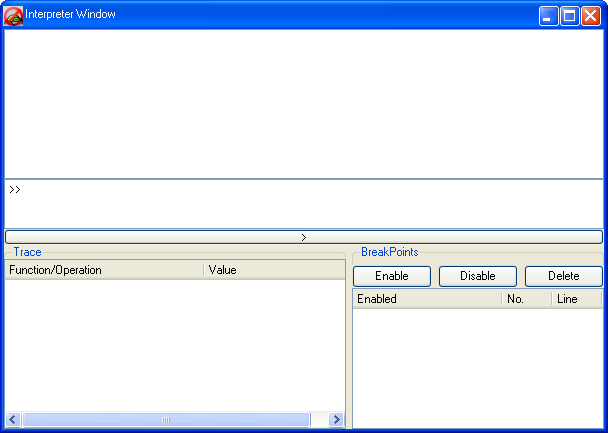
\includegraphics[width=11cm]{interpreterWindowENG.png}
\caption{The Interpreter Window}
\label{fig:interpwin}
\end{center}
\end{figure}

The top two panes of the tool are respectively the
\guicmd{Response} and \guicmd{Dialog} panes: you
can give commands directly to the interpreter in the
\guicmd{Dialog} pane and you receive output from the
interpreter in the \guicmd{Response} pane. To evaluate a \vdmslpp\
expression, you type it directly on the command line in the
\guicmd{Dialog} pane.

Type the following expression into the \guicmd{Dialog} pane:


\begin{verbatim}
  print { a | a in set {1,...,10} & a mod 2 = 0 }
\end{verbatim}

then press RETURN.  The answer is a set of even
numbers. The expression you evaluated was a set comprehension, a value
construction which is explained further in
\ifthenelse{\boolean{VDMsl}}{\cite{UMLMan-SCSK}}{\cite{LangManPP-SCSK}}.

It is also possible to refer to the \vdmslpp\ constructs which have
been read in from the 
\ifthenelse{\boolean{VDMsl}}{{\tt sort-init.rtf} file}{specification
  files}, but before doing this you must first
initialise\index{Interpreter!Initialising} the 
interpreter by pressing the 
\raisebox{-1.0mm}{
\includegraphics[width=0.03\textwidth]{runI.png}}  
(\guicmd{Init}) button. 
During initialisation, constants are 
evaluated and \ifthenelse{\boolean{VDMsl}}{state values}{instance
  variables} are initialised. 
After initialisation you can refer to any of the functions,
operations, \ifthenelse{\boolean{VDMsl}}{}{instance variables,}
values, types etc.\ which are defined in the
\ifthenelse{\boolean{VDMsl}}{}{classes in the} specification.

In order to see which functions\index{Interpreter!Callable Functions}
you can call 
currently, type {\tt functions} at the prompt in the \guicmd{Dialog}
pane and press RETURN. This displays the list of available
functions. From this list you can see that it is, for example,
possible to call the invariant function\index{Invariant Functions|see
  {\\ Functions, \\ Invariant}}\index{Functions!Invariant} for
types which have an invariant attached to them, like the type {\aaa
  PosReal}. The dialogue is illustrated in Figure~\ref{fig:evalgui}.


\begin{figure}[tbh]
\begin{center}
\mbox{}
%\resizebox{0.8\textwidth}{!}{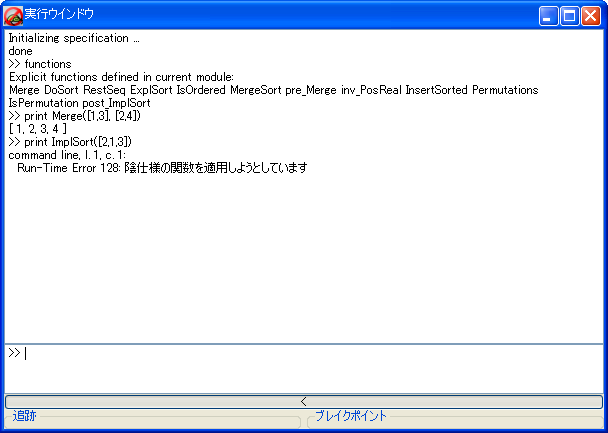
\includegraphics{evalExpr-sl}}
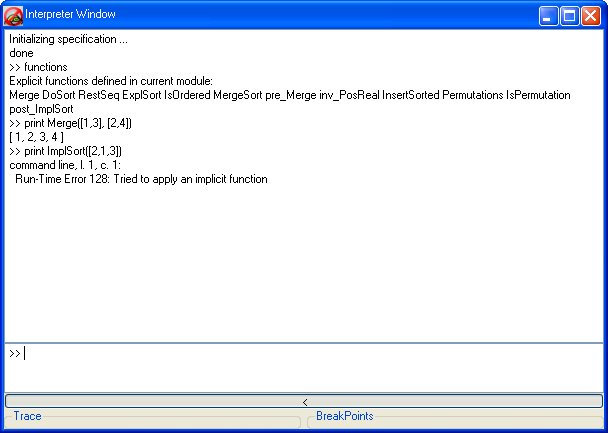
\includegraphics[width=15cm]{evalExpr-slENG.png}
\caption{Evaluation of Expressions}
\label{fig:evalgui}
\end{center}
\end{figure}

Now you can use the {\tt print} command to call, for example, the
{\aaa Merge} function with two ordered sequences of integers (type,
for instance, {\tt print Merge([1, 3], [2, 4])}) and the
interpreter will display the result of evaluating the {\aaa Merge}
function with those particular arguments~({\tt [1, 2, 3, 4]};
see Figure~\ref{fig:evalgui}).

Note that a few \vdmslpp\ constructs are not executable and therefore
cannot be evaluated using the interpreter. For example, if you try
to call the implicitly defined function \index{Implicit
  Functions|see{\\ Functions, \\ Implicit}} \index{Functions!Implicit} {\aaa
  ImplSort}, the interpreter will return an error saying that it
encountered a non-executable construct\index{Non-executable
  Constructs} during evaluation.  See Figure~\ref{fig:evalgui}. 



\subsubsection{Setting breakpoints}
\label{sec:gui-breakpoints}\index{Breakpoints}\index{Breakpoints!Setting} 

Breakpoints cause the interpreter to break execution when evaluating 
functions or operations.

Set a breakpoint in the function \ifthenelse{\boolean{VDMsl}}{{\aaa
MergeSort} by typing {\aaa break MergeSort}}{{\aaa
MergeSorter} in the class {\aaa MergeSort} by typing {\aaa break
MergeSort`MergeSorter}}.

(\ifthenelse{\boolean{VDMsl}}
{
If you are setting a breakpoint in the
current module you can simply refer to the function/operation name.
If you are setting a breakpoint in another module you must qualify the
function/operation name with the name of the module in which it is
defined.
}{When setting a breakpoint the name of the function or
operation must be qualified with the name of the class in which it is
defined.}) The location of the breakpoint will now appear in the
\guicmd{BreakPoints} pane at the bottom right of the
\guicmd{Interpreter Window} together with the number allocated to the
breakpoint (1 in this case since this is the first breakpoint we have
set) and the symbol \raisebox{0.5mm}{{\fbox{\tt\tiny $\surd$}}}\ which
indicates that the breakpoint is enabled.  You can now use the {\cmd
  debug} command\index{debug command} to start the evaluation
instead of the {\cmd print} command\index{print command} used
before. The only difference between the two commands is that {\cmd
  debug} forces the interpreter to stop at breakpoints whereas
{\cmd print} ignores breakpoints.\index{Breakpoints!Ignoring} 

\begin{verbatim}
  debug MergeSort([ 3, 56, 34-12, 0 ])
\end{verbatim}

will cause the interpreter to stop at the breakpoint when it enters
the function \ifthenelse{\boolean{VDMsl}}{{\aaa MergeSort}}{{\aaa
    Sort}}. At the same time, the source file containing the
specification of the function \ifthenelse{\boolean{VDMsl}}{{\aaa
    MergeSort}}{{\aaa Sort}} is displayed in the \guicmd{Source
  Window} and the current point of evaluation (at the moment this is
the location of the breakpoint, i.e.\ the beginning of the function
\ifthenelse{\boolean{VDMsl}}{{\aaa MergeSort}}{{\aaa
    Sort}}) is indicated by the cursor. In addition, the
\guicmd{Trace} pane, which is situated at the bottom left of the
\guicmd{Interpreter Window}, shows the function call stack\index{Call
  stack}.

You can now inspect the values of the parameters of the
    \ifthenelse{\boolean{VDMsl}}{{\aaa MergeSort}}{{\aaa Sort}} 
function, either by printing them using {\cmd print} (e.g.\ by typing
{\aaa print l} in the \guicmd{Dialog} pane)\index{print command}
or by clicking the left mouse button on the \Sig{...} adjacent to
the function name in the \guicmd{Trace} pane at the bottom left of
the \guicmd{Interpreter Window}. Clicking the left mouse button on the
parameters which are revealed will replace them with the \Sig{...}
again.

You can also set breakpoints by selecting the desired position
directly in the appropriate source file. In addition, breakpoints need
not be at the start of a function/operation but can be at any position
within its body.

If the source file is not an RTF file you can set breakpoints by
double-clicking the left or middle mouse button on the desired
position in the file in the \guicmd{Source Window}. If you are using
an RTF source file you must position the cursor at the appropriate
position in the file in Microsoft Word, then press
\texttt{Control-Alt-spacebar} %\index{control-alt-spacebar} 
to set a breakpoint.

You can set breakpoints at any time during debugging, so now use the
source file to set a new breakpoint inside the function {\aaa Merge}
\ifthenelse{\boolean{VDMsl}}{}{in the class {\aaa MergeSort}} as
described above.

Return to the interpreter and press the
\raisebox{-1.0mm}{
\includegraphics[width=0.03\textwidth]{continueI.png}} 
(\guicmd{Continue}) button on the (\guicmd{Interpreter}) toolbar.  
This causes the execution to carry on to the next breakpoint. In fact
because of the recursive call of \ifthenelse{\boolean{VDMsl}}{{\aaa
    MergeSort}}{{\aaa Sort}} the interpreter will stop at the same
breakpoint again, so press the \guicmd{Continue} button repeatedly
until the execution stops inside the {\tt Merge} function.

As the execution proceeds, the various function/operation calls are
logged in the \guicmd{Trace} pane, and you can use this function call
stack\index{Call stack} to navigate through the steps of the
execution so far. Press the 
\raisebox{-1.0mm}{
\includegraphics[width=0.03\textwidth]{upI.png}}  
(\guicmd{Up}) button a couple of times to see how the position in the
function trace context can be changed. The 
\raisebox{-1.0mm}{
\includegraphics[width=0.03\textwidth]{downI.png}}  
(\guicmd{Down}) button can be used to move back down the
trace again.

You can also step through the execution expression by expression by
pressing the 
\raisebox{-1.0mm}{
\includegraphics[width=0.03\textwidth]{singlestepI.png}}
(\guicmd{Single Step}) button. Press this a few times and 
see how the cursor in the \guicmd{Source Window} moves to mark the
changes in the current point of evaluation. You now have access not
only to the parameters of the function but also to all the variables
(including local variables) that are in scope at the current point of
evaluation, and you can inspect their values using, for example, the
{\cmd print} command.

This debugging is shown in Figure~\ref{fig:guidebug}.  


\begin{figure}[tbh]
\begin{center}
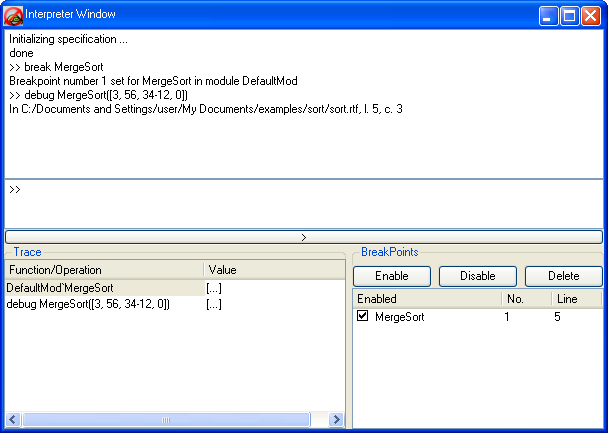
\includegraphics[width=\textwidth]{debugging-slENG.png}
\caption{Debugging a Specification}

\label{fig:guidebug}
\end{center}
\end{figure}

You can delete breakpoints, also at any time during the
debugging.\index{Breakpoints!Deleting} Try this by typing 
{\tt delete 1} (i.e.\ delete breakpoint number 1) in the
\guicmd{Dialog} pane of the \guicmd{Interpreter Window}. Selecting the
breakpoint in the \guicmd{BreakPoints} pane of the \guicmd{Interpreter
  Window} and pressing the \guicmd{Delete} button at the top of that
pane has the same effect.

The other two buttons at the top of the \guicmd{BreakPoints} pane are
for enabling and disabling
breakpoints.\index{Breakpoints!Disabling}\index{Breakpoints!Enabling}
Set the breakpoint in the function \ifthenelse{\boolean{VDMsl}}{{\aaa
    MergeSort}}{{\aaa MergeSort`MergeSorter}} again, then select
it in the \guicmd{BreakPoints} pane and press the \guicmd{Disable}
button. Note how the symbol \raisebox{0.5mm}{{\fbox{\tt\tiny
      $\surd$}}}\ is replaced by the symbol
\raisebox{1mm}{{\fbox{\rule[-0.75mm]{0mm}{1.5mm}{\hspace*{1.5mm}}}}}\
to indicate that the breakpoint is disabled. Pressing the
\guicmd{Enable} button will re-enable the breakpoint and the symbol
will change back to \raisebox{0.5mm}{{\fbox{\tt\tiny $\surd$}}}\ to
confirm this.


% It is also possible to make
% nested debugs.\index{Debugging!Nested} Try doing this and try using the
% {\tt popd}\index{{\tt popd} command} command to restore the context
% that existed when the last {\tt debug} command was invoked.

\subsubsection{Dynamic type checking}
\index{Type Checking!Dynamic}

Although the type checker reported no errors in our specification,
there may still be type errors because in general it is not possible
to find all type errors by a simple static analysis of type
information (i.e.\ an analysis based only on the types declared in the
signatures of functions and operations). Thus, for example, if a
function is declared as taking an integer (of type {\aaa int}) as its
argument but is applied to an expression which evaluates to a real
number (of type {\aaa real}) this will not raise a static type error
because {\aaa int} is a subtype of {\aaa real} so the application
might be correct provided the function is called at run-time with
parameters which are actually integer reals.

In order to help discover this kind of type error at the specification
level, the interpreter can be configured to perform dynamic type
checking during evaluation.  This option is enabled through the
\guicmd{Interpreter} pane of the \guicmd{Project Options} window, 
which is displayed by pressing the
\raisebox{-1.0mm}{
\includegraphics[width=0.03\textwidth]{projectoptions.png}} 
(\guicmd{Project Options}) button on the (\guicmd{Project Operations})
toolbar. This is shown in Figure~\ref{fig:interoptions}.

\begin{figure}[tbh]
\begin{center}
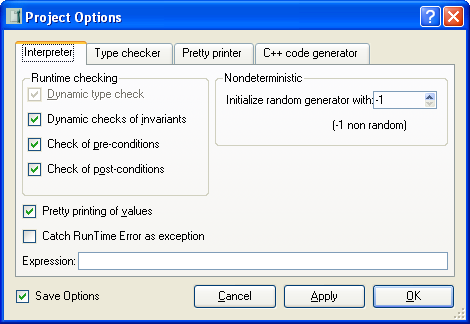
\includegraphics[width=12.5cm]{interpreterOptions-slENG.png}
\caption{Setting Interpreter Options}
\label{fig:interoptions}
\index{Options!Interpreter}
\end{center}
\end{figure}

Enabling dynamic type checking causes the interpreter to check actual
types during an evaluation.

To see an example of this, enable dynamic type checking by selecting
it in the \guicmd{Interpreter} pane of the \guicmd{Project Options}
window and pressing the \guicmd{OK} button to accept the new
options. Then evaluate the expression 


\begin{verbatim}
  debug MergeSort([ 3.1415, -56, 34-12, 0 ])
\end{verbatim}


again in the \guicmd{Dialog} pane. This time the interpreter reports a
dynamic type error. (If you have not deleted or disabled all
breakpoints you will need to step through the specification to see
this.) This is because according to its signature the function
\ifthenelse{\boolean{VDMsl}}{{\aaa Merge}}{{\aaa MergeSort`Merge}}
expects sequences of integers as its parameters whereas the actual
parameters contain the value {\tt 3.1415} which is not an integer but
a real number. This dynamic type error thus reveals a possible error
in the specification -- the top-level function {\aaa MergeSort}
\ifthenelse{\boolean{VDMsl}}{}{ in the {\aaa MergeSorter} class} can
accept sequences of real numbers as its parameters but it calls the
function {\aaa Merge} \ifthenelse{\boolean{VDMsl}}{}{in the same
    class} which is only defined for lists of integers.

In a similar way, the interpreter can be configured to dynamically
check that invariants on types and preconditions and postconditions of
functions and operations are respected (i.e.\ evaluate to {\aaa true})
during evaluation. These options are also enabled through the
\guicmd{Interpreter} pane of the \guicmd{Project Options} window 
shown in Figure~\ref{fig:interoptions}.\index{Precondition Checking}
\index{Postcondition Checking}\index{Invariant Checking}

As an example, return to the \guicmd{Interpreter} pane of the
\guicmd{Project Options} window and enable the option \guicmd{Check of
  pre-conditions}. Now evaluate the previous expression again but this
time omitting the number {\tt 3.1415} from the list. Now the
interpreter reports a precondition violation as shown in
Figure~\ref{fig:dtcerror}. This is because the precondition of the
function \ifthenelse{\boolean{VDMsl}}{{\aaa Merge}}{{\aaa
    MergeSort`Merge}} requires that all the input values 
should be non-negative.

\begin{figure}[tbh]
\begin{center}
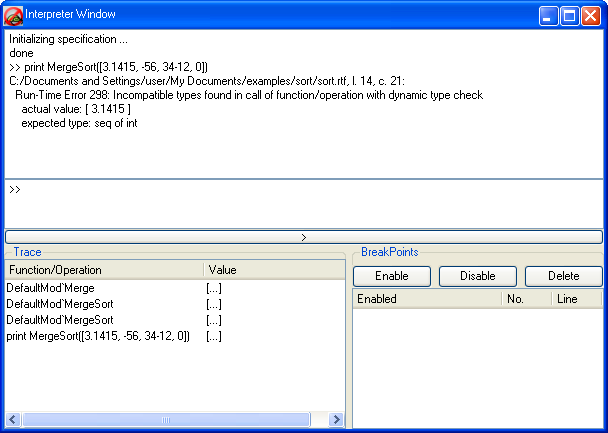
\includegraphics[width=12.5cm]{dynamicTCError-slENG.png}
\caption{Dynamic Type Checking Error}
\label{fig:dtcerror}
\end{center}
\end{figure}

\subsubsection{Checking Integrity Properties}\label{pogWalk}
\index{Integrity Properties}

Dynamic checking of types, invariants, preconditions and
postconditions as described above is basically one form of testing --
it checks for run-time errors for some \emph{specific} input
values. The integrity examiner offers a more general way of
investigating possible run-time errors, though it is perhaps less
intuitive for people who are more familiar with programming than with
mathematics.

The integrity examiner analyses the specification looking for places
where run-time errors could potentially occur and generates a series
of integrity properties which represent conditions under which no
run-time errors should occur. These integrity properties are more
general than dynamic checking because they are presented as
 \vdmslpp\ predicates that involve quantification over all
possible values of the appropriate variables\footnote{In some cases
  the full context is not shown explicitly and the scope of some
  variables has to be determined by inspection of the specification.},
which means that if it 
can be demonstrated that an integrity property is true there will
not be run-time errors associated with that integrity check whatever
the values of the variables involved (dynamic checking of course
only checks that there are no run-time errors for the particular
values of the variables chosen). Of course if an integrity property
can instead be shown to be false this would point to there being a
potential problem with the corresponding part of the specification.

To see how the integrity examiner works in practice, select the 
\ifthenelse{\boolean{VDMsl}}{{\aaa DefaultMod} module}{ {\aaa
    ExplSort} class} then invoke the integrity examiner for this
\ifthenelse{\boolean{VDMsl}}{module}{class} by pressing the 
\raisebox{-1.0mm}{
\includegraphics[width=0.03\textwidth]{integritycheck.png}}  
(\guicmd{Generate Integrity Properties}) button on the (\guicmd{Actions})
toolbar. The \guicmd{Integrity Properties Window} then opens and
displays the integrity properties generated. This is shown in 
Figure~\ref{fig:integWin}.


\begin{figure}[tbh]
\begin{center}
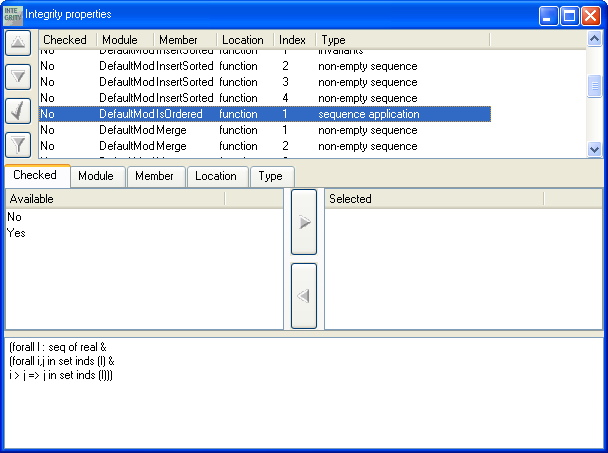
\includegraphics[width=12.5cm]{integWin-slENG.png}
\caption{The Integrity Properties Window}
\label{fig:integWin}
\end{center}
\end{figure}

The top pane of the \guicmd{Integrity Properties Window} shows a list
of the integrity properties together with information about their
status (the \guicmd{Checked} column), their position in the specification (the
\guicmd{Module}, \guicmd{Member} and \guicmd{Location} columns) and
their type (the \guicmd{Type} column). The numbers in the
\guicmd{Index} column simply serve to distinguish different integrity
properties which have the same position. As can be seen from this
example, even a small specification can generate many integrity
properties -- in fact thirty different types of integrity properties
are checked in all -- so in a large specification it is useful to be
able to filter these. The middle two panes of the \guicmd{Integrity
  Properties Window} offer various filtering
methods\ifthenelse{\boolean{VDMsl}}{}{ (see Section~\ref{sec:pog} for
  details)}. Finally, if a particular integrity 
property is selected in the top pane of the window the corresponding
\vdmslpp\ predicate is displayed in the bottom pane of the window, and
at the same time the cursor in the \guicmd{Source Window} indicates
the exact point in the specification to which the selected integrity
property relates. Each integrity property can thus be inspected in
order to try to determine whether or not it is true.


Select the \guicmd{Member} attribute in the left-hand pane of the
middle pane of the window, then select the four functions
\guicmd{ExplSort}, \guicmd{IsOrdered}, \guicmd{Permutations}, and
\guicmd{RestSeq} in the same pane and press the
\raisebox{-1.0mm}{
\includegraphics[width=0.03\textwidth]{right.png}}  
(\guicmd{Add to Filter}) button to add them to the filter. Pressing the 
\raisebox{-1.0mm}{
\includegraphics[width=0.03\textwidth]{filter.png}}  
(\guicmd{Filter}) button on the left-hand side of the top pane of
the window then causes the list of integrity properties to be filtered
to show only those which relate to these functions.


Select the first (i.e.\ index number 1) integrity property relating to
the function {\aaa isOrdered}. This has the form:


\begin{verbatim}
  (forall l : seq of real &
  (forall i,j in set inds (l) &
  i > j =>
   i in set inds (l)))
\end{verbatim}


and, as can be seen from the position of the cursor in the
\guicmd{Source Window}, corresponds to the condition that the sequence
application \verb+l(i)+ in the expression

\begin{verbatim}
  forall i,j in set inds l & i > j => l(i) >= l(j)
\end{verbatim}

must be well-defined, i.e.\ the value {\aaa i} must always belong to the
indices of the sequence {\aaa l}.

In this particular case it is in fact easy to see that the integrity
property is true -- the second quantification in the predicate
directly tells us that both {\aaa i} and {\aaa j} belong to the
indices of {\aaa l}, and whether or not {\aaa i} is bigger than {\aaa
  j} (the third line of the predicate) is irrelevant. The property can
therefore be marked as having been checked, which is done by pressing
the
\raisebox{-1.0mm}{\includegraphics[width=0.03\textwidth]{checkmark.png}}  
(\guicmd{Toggle Status}) button to the left of the top pane of the
\guicmd{Integrity Properties Window}.

Now look at the other three integrity properties related to sequence
application. It is also easy to see that these are true: the one
relating to {\aaa isOrdered} is exactly analogous to the one discussed
above except that it relates
to the sequence application \verb+l(j)+ rather than to \verb+l(i)+, so
the same argument applies; the one relating to {\aaa
  Permutations} is immediately true because the second quantification
gives exactly the result required (\verb+i in set inds (l)+); and in
the case of {\aaa RestSeq} the third quantification tells us that
{\aaa j} belongs to the indices of {\aaa l} with {\aaa i} removed
which means that {\aaa j} must belong to the indices of {\aaa
  l}. These three integrity properties can therefore be selected and
marked as checked in the same way.

In cases such as these, the integrity properties could in fact be
verified automatically by a mechanical checker. However, this is not
always possible and in the more complicated cases the reasoning
process needs to be steered by a human even though the actual
reasoning can be mechanised.

%\footnote{A prototype automatic checker and
%  reasoning support system has in fact been produced but this is not
%  yet sufficiently developed for full integration with the
%  Toolbox.}. 

One such more complicated property is the one relating to the 
\ifthenelse{\boolean{VDMsl}}{{\aaa ExplSort} function}{{\aaa
  Sort} operation}, which basically states that there must be at least
  one value {\aaa r} which satisfies the predicate in the implicit
  {\aaa let} statement otherwise the specification does not make
  sense\ifthenelse{\boolean{VDMsl}}{}{\footnote{There is an implicit
      quantification here over the variable {\aaa l} which, according
      to the specification, is an arbitrary sequence of
      integers.}}. It is not so easy to see that this 
  property is true because it involves three user-defined functions
  -- {\aaa Permutations}, {\aaa isOrdered}, and {\aaa RestSeq} which
  is used in the definition of {\aaa Permutations} -- and in
  addition {\aaa Permutations} is defined recursively. However, it is
  easy to see that the integrity property is true \emph{provided} the
  functions {\aaa Permutations} and {\aaa isOrdered} are defined
  correctly -- clearly it is possible to sort any given sequence of
  numbers, so we just need to be sure that the set of sequences
  returned by the function {\aaa Permutations} comprises all possible
  permutations of the input sequence and that the function {\aaa
  isOrdered} defines ordered sequences of numbers correctly.

Look at the definition of the function {\aaa isOrdered} in the
\guicmd{Source Window}. It is relatively easy to see that this is
correct -- its defining predicate states directly that, given any two
positions in the sequence, the number at the later position cannot be
smaller than the number at the earlier position, and this clearly
means that the elements must be in (ascending) order.

Now look at the function {\aaa Permutations}. The first branch of the
cases expression is easy 
to deal with -- there is only one possible permutation of the empty
sequence and sequences with only one element, namely the sequence
itself. For the {\aaa others} branch, we first need to look at the
function {\aaa RestSeq}. It is fairly easy to see that this simply
removes the element at a given position from a given sequence. In the
{\aaa others} branch of the function {\aaa Permutations}, therefore,
we are constructing permutations by choosing an arbitrary element from
the original sequence as the first element of the permutation and
concatenating all possible permutations of the remaining elements of
the original sequence onto this. This therefore gives us all possible
permutations, so the integrity property is satisfied.

Looking now at the remaining two integrity
properties\ifthenelse{\boolean{VDMsl}}{}{, both} relating to the 
function {\aaa RestSeq}, it is easy to see that the one of type {\aaa
  Postcondition}, which requires that the explicit result of the
function satisfies the postcondition if the precondition is satisfied,
is valid -- the function removes one element from the sequence so the
length of the sequence is reduced by one and the elements of the
sequence are either unchanged (in the case when the element removed
occurs more than once in the sequence) or smaller. However, the
property of type {\aaa Invariant} states that every natural number is
different from zero, and this is of course false.

Looking at the specification of {\aaa RestSeq} in the \guicmd{Source
  Window}, you can see that the property is generated by the
  precondition of the function:

\begin{verbatim}
  i in set inds l
\end{verbatim}

In fact it arises because the indices of a sequence is a set of
positive natural numbers (i.e.\ is of type 
\verb+set of nat1+) so that if {\aaa i} is not of type {\aaa nat1} the 
precondition will automatically be false. This indicates that the
{\aaa nat} in the signature of the function should be changed to {\aaa
  nat1}. If this is done, the new integrity property will be 

\begin{verbatim}
  (forall l : seq of real, i : nat1 &
  i <> 0)
\end{verbatim}


and this is of course true.

Finally, look at the last integrity property, the invariant property
for the function \guicmd{ExplSort}. This has the form
\begin{verbatim}
  (forall l : seq of PosReal &
  (forall xx_10 in set elems (let r in set Permutations(l) be st 
    isOrdered(r) in r ) &
  DefaultMod`inv_PosReal(xx_10)))
\end{verbatim}

This looks quite complicated but in fact it just states that if we
start with a sequence of positive real numbers and order the sequence
then every number in the resulting sequence satisfies the invariant on
the type {\aaa PosReal}, i.e.\ is also a positive real number. This is
clearly true so this property can also be marked as checked.

The integrity properties for the other
\ifthenelse{\boolean{VDMsl}}{functions}{classes} can be dealt with in
a similar way.




\subsection{Introducing Systematic Testing}
\label{tour:testing}

As part of its support for validation, the \Toolbox\ provides a
facility for testing \vdmslpp\ specifications, including test
  coverage measurement.\index{Test
  Coverage}  Test coverage measurement helps you to see
how well a given test suite\index{Test Coverage!Test suite} covers the
specification. This is done by collecting information in a special
test coverage file about which statements and expressions are
evaluated during the execution of the test suite.

There are three steps involved in producing a test coverage report:


\begin{enumerate}
\item
Prepare a {\em test coverage file}\index{Test
Coverage!File}. This file contains
  information about the specification's structure. 
\item Test the specification by making the interpreter execute calls
to the constructs in the specification. This process updates the test
coverage information in the test coverage file.
\item Pretty print the test coverage report: the pretty printer takes
  the specification and test coverage files and produces a nicely typeset
  version of the specification with test coverage information
  included. We will return to this part below in Section~\ref{subsec:pp}.

\end{enumerate}

\begin{figure}[tbh]
\begin{center}
\includegraphics[width=12.5cm]{testCov-slENG.png}
\caption{Collecting Test Coverage Information}
\label{fig:guitcov}
\end{center}
\end{figure}

This process is illustrated in Figure~\ref{fig:guitcov}. First the 
{\tt tcov reset}\index{tcov reset command} is issued to
reset the test coverage file so that it has no information about any
prior testing carried out for the given specification. Then the
\guicmd{print} command is used to evaluate different constructs from
the specification. The command \guicmd{tcov write}\index{tcov
  write command} then saves all the test coverage information
generated since the last \guicmd{tcov reset} command to the file
\texttt{vdm.tc}. Finally, the command \guicmd{rtinfo}\index{rtinfo command} 
displays a table summarising the information in
this test coverage 
file. This consists of a list of the various functions and operations
in the specification together, each annotated with the number of times
that function/operation has been called during testing and the
percentage of its specification which has been tested at least once.

Note that the command-line version of the \vdmslpp\ \Toolbox\ 
(\ifthenelse{\boolean{VDMsl}}{\texttt{vdmde}}{\texttt{vppde}}) also
has facilities to support the collection of test coverage
information.

Naturally realistic testing would involve many more tests before the
information is written to the test coverage file \texttt{vdm.tc} using the
\guicmd{tcov write} command. Indeed, for
real projects you would generally set up an entire test environment 
where you make a small script file which automates this whole
process. This can also compare the actual results of individual tests
against expected results (it is necessary to use the {\tt -O} option
for this).  Appendix~\ref{sec:testscript} contains an example of such
a script file for both Windows and Unix.


\subsection{Pretty Printing}\label{subsec:pp}

\index{Pretty Printing}
%\index{generating \LaTeX|see{pretty printing}}
%\index{latex@\LaTeX|see{pretty printing}}

The pretty printer transforms a specification from its input format to
a pretty printed version of the specification. Typically this pretty
printed version is used for documentation purposes.

In order to see pretty printing at work, first go to the \guicmd{Pretty
Printer} pane of the \guicmd{Project Options} window and enable one of the
options to produce indexes (it does not matter which of the 
two options you choose when the RTF format is used) and also the test
coveraging colouring option. You also need to copy the {\tt vdm.tc}
file you have just produced to the working directory of the
\Toolbox, which you can determine using the {\tt pwd}\index{pwd command}
which you can run in the \guicmd{Dialog} pane of the
interpreter\footnote{If the project you are working on has been saved
  then the directory in which it was saved will be the working
  directory.}.

Select \ifthenelse{\boolean{VDMsl}}{the {\tt sort-init.rtf} file}{all
six {\tt .rtf} files} in the \guicmd{Project View} in the
\guicmd{Manager}, then press the % should this work in VDM/Module Views? 
\raisebox{-1.0mm}{\includegraphics[width=0.03\textwidth]{prettyprint.png}}
(\guicmd{Pretty Print}) button on the
(\guicmd{Actions}) toolbar. In the \guicmd{Log Window} you will
see that this produces \ifthenelse{\boolean{VDMsl}}{a file {\tt
sort-init.rtf.rtf}}{a {\tt .rtf.rtf} file for each of the selected
input files}. Start Microsoft Word on the
\ifthenelse{\boolean{VDMsl}}{{\tt sort-init.rtf.rtf}}{{\tt dosort.rtf.rtf}}
file. Notice how all the \vdmslpp\ keywords have been converted to
boldface type. The
other parts of your specification have been typeset using the Word
styles {\tt VDM\_COV} and {\tt VDM\_NCOV} which relate to the covered
and non-covered parts respectively. The definition of these styles can
be changed and unless you use a colour printer for your documents it
is necessary to modify the definition of the {\tt VDM\_NCOV} style
(e.g.\ by using grey for the non-covered parts).

Go to the bottom of the \ifthenelse{\boolean{VDMsl}}{{\tt
sort-init.rtf.rtf}}{{\tt dosort.rtf.rtf}} file. Note how the
text written in the {\tt VDM\_TC\_TABLE} style has been replaced with a
table showing the test coverage statistics. The three columns give
respectively the name of the function/operation, the number of calls
of that construct in 
the test coverage file, and the percentage coverage for it. The table
looks like\footnote{Note that this is quite similar to part of the
information we saw directly inside the \guicmd{Response} pane of
the interpreter in the previous section.}:


\begin{center}
\begin{tabular}{|l|r|r|}\hline
\textbf{name}   & \textbf{\#calls} & \textbf{coverage} \\ \hline
DoSort          & 4     & 100\% \\
ExplSort        & 0     & 0\%\\
InsertSorted    & 3     & 62\%\\
IsOrdered       & 0     & 0\%\\
IsPermutation   & 0     & 0\%\\
Merge           & 0     & 0\%\\
MergeSort       & 0     & 0\%\\
Permutations    & 0     & 0\%\\
RestSeq         & 0     & 0\%\\
\textbf{total}  &       & 15\%\\\hline
\end{tabular} 
\end{center}

Finally, go to the end of the file and select the \guicmd{Index
and Tables ...} item from the \guicmd{Insert} pull down menu inside
Microsoft Word. Decide the layout you wish to use for the index
overview of the definitions in the \ifthenelse{\boolean{VDMsl}}{{\tt
sort-init.rtf.rtf}}{{\tt dosort.rtf.rtf}} file. Press \guicmd{Ok} and see how
an index of VDM definitions can be created automatically.

Using the alternative pretty printing mechanisms with \LaTeX\ is quite
different but this is explained in the reference section of this
manual (see Section~\ref{sec:testing}).


\subsection{Generating Code}
\index{C++ Code Generation}
\index{Code Generation|see {\\ C++ Code Generation, \\ Java Code Generation}}

If you have a license \index{License} for the \vdmslpp\ to C++
Code Generator you can automatically have your specification
translated into C++ code by pressing the 
\raisebox{-1.0mm}{\includegraphics[width=0.03\textwidth]{cplusplus.png}}
(\guicmd{Generate C++}) button. See
\ifthenelse{\boolean{VDMsl}}{\cite{CGMan-SCSK}}{\cite{CGManPP-SCSK}} for further
information about the C++ Code Generator.



\subsection{The Dynamic Link Facility}\index{Dynamic Link Facility}

Another additional feature which needs a special license
\index{License} is 
called the Dynamic Link facility. This feature
enables you to interpret a 
combination of a system which is partly specified in \vdmslpp\ and is
partly present in C++ code\index{C++ Files}. This feature is not
illustrated by the sort example, but it is illustrated in
\cite{DLMan-SCSK}. Also see \cite{DLMan-SCSK}
for further information about the Dynamic Link facility.


\subsection{The \protect\VDMTools\ API}

All of the functionality of \VDMTools\ is exposed to external programs
via a Corba-compliant application programmers interface (API). Details
of how to use this API may be found in \cite{APIMan-SCSK}.


%\subsubsection{Display of test coverage information in the GUI} \label{guirti}

%The tool \texttt{Test Coverage Tool} in the GUI can be used for
%displaying the collected test coverage information. The tool should be
%opened, the file for which test coverage information is wanted should
%be selected, and the button \texttt{Show Coverage} should be pressed.
%The specification file will be shown in the display window with the
%uncovered expressions and statements marked on the leading character
%with a red background (or underlined for B\&W displays).

\subsection{Exiting \protect\VDMTools}

When you wish to exit the \Toolbox\ you should select the
\guicmd{Exit} item on the \guicmd{Project} menu in
the main window. If you exit without saving the project, a dialog
window will appear asking if you want to save your project.

This completes the guided tour of the \Toolbox. We hope that you now have
a better understanding of the kind of fuctionality it can provide. Now
you should be able to start using the \Toolbox\ for your own
\vdmslpp\ models. The remaining parts of this manual are a detailed
reference guide providing more details about particular features.


\newpage
\section{The \protect\VDMTools\ Reference Manual}\label{sec:ref}

This section is structured into a number of subsections covering each
of the tools in the \Toolbox. For each tool, its use through each of
the three interfaces (the graphical user interface, the Emacs
interface and the command line interface) is described.


\subsection{The Overall Graphical User Interface}\label{sec:GUI}
\index{Graphical User Interface}\index{Graphical User Interface!Starting}

The graphical user interface to the \Toolbox\ is started by selecting
it from the programs entry in the Windows setup under Windows or with
the command {\tt \vdmgde}\index{vdmgde command} on Unix platforms.
This opens the main graphical user interface window, which is shown in 
Figure~\ref{fig:startgui2}. 


\begin{figure}[tbh]
\begin{center}
\includegraphics[width=11cm]{startgui-slENG.png}
\caption{Graphical User Interface Startup}
\label{fig:startgui2}
\end{center}
\end{figure}

The top of this window consists of a menu line with six pull-down
menus, below which are six toolbars \footnote{When the \Toolbox\ is
  started, only three toolbars are displayed open, the other three
  being displayed in iconised form above them.} comprising buttons
which offer the same actions as the menus \footnote{Except that the
  function for exiting from the toolbox is only available on the
  \guicmd{Project} menu.}. The bottom part of the window is used to
display various subwindows which either present information about the
status of the current project or offer interfaces to tools within the
\Toolbox. We describe each of the menus/toolbars and the available
subwindows, grouped according to functionality, in the following
subsections.

\subsubsection{Project handling}\index{Project}
A project consists of a collection of files that together form a
\vdmslpp\ specification. Projects can be saved to and read from disk,
which means that you do not need to configure the \Toolbox\ with the
individual files every time you wish to use it: you simply
open the relevant project file. Projects are only available in the
graphical user interface.

The \guicmd{Manager}\index{Manager}, which is opened/closed by
pressing the 
\raisebox{-1.0mm}{\includegraphics[width=0.03\textwidth]{browser.png}}
button on the \guicmd{Window Operations} toolbar or by
selecting the appropriate item from the \guicmd{Windows} menu,
displays the current status of the current
project and is also  the place where you select which subset of
project files you want the various \Toolbox\ operations to be applied
to. It consists of two parts: the \guicmd{Project View} and the
\ifthenelse{\boolean{VDMsl}}{\guicmd{Module View}}{\guicmd{Class
      View}}.

The \guicmd{Project View} displays a tree representation of the contents
of the project comprising the files in the project and (only after
successfully syntax checking the file) the
\ifthenelse{\boolean{VDMsl}}{modules}{classes} declared in each file. 
It is shown in Figure~\ref{fig:projectView}.


\begin{figure}[tbh]
\begin{center}
\mbox{}
\includegraphics[width=9cm]{projectView-slENG.png}
\caption{The Project View}
\label{fig:projectView}
\end{center}
\end{figure}


When \vdmslpp\ files have been successfully syntax checked the names
of the \ifthenelse{\boolean{VDMsl}}{modules}{classes} defined in those
files are listed in the \vdmModView. This view also displays the
status of each of the individual 
\ifthenelse{\boolean{VDMsl}}{modules}{classes} in the project: the
symbols 
\raisebox{-0.7mm}{\includegraphics[width=0.03\textwidth]{syntaxcheckdone.png}},
\raisebox{-1.0mm}{\includegraphics[width=0.03\textwidth]{typecheckdone.png}},
\raisebox{-1.0mm}{\includegraphics[width=0.03\textwidth]{cplusplusdone.png}},
and
\raisebox{-1.0mm}{\includegraphics[width=0.03\textwidth]{prettyprintdone.png}}
in the appropriate columns indicate respectively that the
\ifthenelse{\boolean{VDMsl}}{module}{class} has been successfully
syntax checked, type checked, translated to C++,
\ifthenelse{\boolean{VDMsl}}{}{translated to Java,} and pretty
printed;
similarly, the corresponding symbols with a (red) line through them (%
\raisebox{-0.7mm}{\includegraphics[width=0.03\textwidth]{syntaxcheckerror.png}},
\raisebox{-1.0mm}{\includegraphics[width=0.03\textwidth]{typecheckerror.png}},
\raisebox{-1.0mm}{\includegraphics[width=0.03\textwidth]{cpluspluserror.png}},
and
\raisebox{-1.0mm}{\includegraphics[width=0.03\textwidth]{prettyprinterror.png}})
indicate that the particular action failed. Note that a blank in a
column means that no attempt has yet been made to perform that
particular action. Note also that if one of the files in the project
is modified on the file system the symbol
\raisebox{-0.7mm}{\includegraphics[width=0.03\textwidth]{syntaxcheckmodified.png}}
is displayed in the \guicmd{Syntax} column  to indicate
that there is an inconsistency between the version currently in the \Toolbox\ and the
version on the file system and that the file should be syntax checked
again before proceeding.



Various operations for manipulating projects, including opening and
saving projects, adding files to and removing files from projects, and
creating new projects, are available from the \guicmd{Project}
menu and the corresponding \guicmd{Project
  Operations} toolbar, which are
shown in Figure~\ref{fig:projectMenuToolbar}.


\begin{figure}[tbh]
\begin{center}
\mbox{}
\includegraphics[width=11cm]{projectMenuToolbar-sl.png}
\caption{The Project Menu and Project Operations Toolbar}
\label{fig:projectMenuToolbar}
\end{center}
\end{figure}

The same menu/toolbar also offer facilities for setting options
relating to the \Toolbox\ environment, for setting options for the
various tools within the \Toolbox, and for exiting the \Toolbox\
(only available on the menu). In more  detail, the available actions
are as follows:


\begin{description}

\item[\guicmd{New Project} (\hspace{-1.8mm}
\raisebox{-0.8mm}{\includegraphics[width=0.03\textwidth]{projectnew.png}}):]
Select this item if you are currently working on 
  a \vdmslpp\ project and you would like to start working on a new
  one.

\item[\guicmd{Load Project ...} (\hspace{-1.2mm}
\raisebox{-0.8mm}{\includegraphics[width=0.03\textwidth]{load.png}}\hspace{.6mm}):]
Select this item if you wish to open an already 
  existing project. A file browser will appear and you can select the
  desired project file. When it has been loaded the \Toolbox\ will
  automatically syntax check all the files in the project.

\item[\guicmd{Save Project} (\hspace{-1.8mm}
\raisebox{-0.8mm}{\includegraphics[width=0.03\textwidth]{projectsave.png}}):]
  Use this item if you have changed the 
  configuration of your current project and want to save the new
  configuration.

\item[\guicmd{Save Project As ...} (\hspace{-1.5mm}
\raisebox{-0.8mm}{\includegraphics[width=0.03\textwidth]{projectsaveas.png}}):]
  Use this item to save your current 
  configuration under a different name. A file browser will appear and
  you can place the new project file where you like and give it the
  name you prefer.

\item[\guicmd{Add File to Project ...} (\hspace{-1.5mm}
\raisebox{-0.8mm}{\includegraphics[width=0.03\textwidth]{plus.png}}):] 
  Use this to add files to the
  project  the \Toolbox\ is currently working with. A window like the
  one shown in Figure~\ref{fig:addFiles} will appear allowing you to
  select the appropriate files. 

\item[\guicmd{Remove File from Project} (\hspace{-1.5mm}
 \raisebox{-0.8mm}{\includegraphics[width=0.03\textwidth]{minus.png}}):]
 Use this to remove files from
 the current project. A dialog box will appear asking you to confirm
 the removal. 

\item[\guicmd{Project Options ...} (\hspace{-1.5mm}
\raisebox{-0.8mm}{\includegraphics[width=0.03\textwidth]{projectoptions.png}}):].
  This opens the \guicmd{Project Options} window, which allows various options
  to be set for the following elements of the \Toolbox:
  \index{Options!Project}
  \begin{itemize}
    \item \guicmd{interpreter} (described in
  Section~\ref{sec:interpreter});
    \item \guicmd{type checker}  (described in Section~\ref{sec:tc});
    \item \guicmd{pretty printer}  (described in Section~\ref{sec:pp});
    \item \guicmd{C++ code generator} (described in Section~\ref{sec:cg})%

% Nothing...
  \end{itemize}

\item[\guicmd{Tool Options ...} (\hspace{-1.5mm}
\raisebox{-0.8mm}{\includegraphics[width=0.03\textwidth]{tooloptions.png}}):].
  This opens the \guicmd{Tool Options} window, which allows various
  environment variables and interface options to be set for the
  \Toolbox\ as a whole. These options are described in
  Appendix~\ref{sec:set_env}. \index{Options!Tool}

\item[\guicmd{Recent Projects}:]
  This opens a list of the recent projects that have been used on the
  computer.

\item[\guicmd{Exit}:] Choose this item to leave the \Toolbox. If you
  have not already saved your project the \Toolbox\ will ask whether
  you wish to do so. Note that this action is not available on the
  toolbar. 


\end{description}

\subsubsection{Operations on specifications}

The \Toolbox\ offers a range of functions which can be applied to a
specification: syntax checking; type checking; generating integrity
properties; generating C++
\ifthenelse{\boolean{VDMsl}}{}{or Java} code;
\ifthenelse{\boolean{VDMsl}}{}{translation from Java to \vdmslpp;} and
pretty printing. These are invoked through the \guicmd{Actions} menu
or the corresponding \guicmd{Actions} toolbar, which are
illustrated in Figure~\ref{fig:actionsMenuToolbar}.


\begin{figure}[tbh]
\begin{center}
\mbox{}
\includegraphics[width=11cm]{actionsMenuToolbar-slENG.png}
\caption{The Actions Menu and Toolbar}
\label{fig:actionsMenuToolbar}
\end{center}
\end{figure}

Each action is applied to every
file/\ifthenelse{\boolean{VDMsl}}{module}{class} which is currently
selected in the \guicmd{Manager}, though the actions are to a certain
extent interdependent so that some of them can only be carried out 
 when the selected \ifthenelse{\boolean{VDMsl}}{modules}{classes} have
 a status which enables the desired functionality to be applied. For
 example, the type checker and the pretty printer features are 
enabled only when the \ifthenelse{\boolean{VDMsl}}{module}{class} has
been accepted by the syntax checker.

The various actions are described in more detail in later sections as follows:


\begin{description}

\item[\guicmd{Syntax Check} (\hspace{-1.8mm}
\raisebox{-0.8mm}{\includegraphics[width=0.03\textwidth]{syntaxcheck.png}}):] see Section~\ref{sec:parser} 

\item[\guicmd{Type Check} (\hspace{-1.8mm}
\raisebox{-0.8mm}{\includegraphics[width=0.03\textwidth]{typecheck.png}}):] see Section~\ref{sec:tc} 

\item[\guicmd{Generate Integrity Properties} (\hspace{-1.8mm}
\raisebox{-0.8mm}{\includegraphics[width=0.03\textwidth]{integritycheck.png}}):] see Section~\ref{sec:pog} 

\item[\guicmd{Generate C++} (\hspace{-1.8mm}
\raisebox{-0.8mm}{\includegraphics[width=0.03\textwidth]{cplusplus.png}}):] see Section~\ref{sec:cg} 


\item[\guicmd{Pretty Print} (\hspace{-1.8mm}
\raisebox{-0.8mm}{\includegraphics[width=0.03\textwidth]{prettyprint.png}}):] see Section~\ref{sec:pp}




\end{description}

\subsubsection{The log window, error list and source window}

The \guicmd{Log Window} displays messages from the \Toolbox, including
messages reporting on the success or failure of applying the actions
described above. It opens automatically (if it is not already open)
when a new message is displayed. Alternatively, it can be
opened/closed by hand by pressing the 
\raisebox{-0.8mm}{\includegraphics[width=0.03\textwidth]{log.png}}
button on the \guicmd{Window Operations} toolbar or by
selecting the corresponding item from the \guicmd{Windows} menu.

%   The \guicmd{Log Window} has three icons:
%   \begin{list}{}{}
%   \item[\includegraphics{clearBig}] This erases the content of the
%     log window.
%   \item[\resizebox{1cm}{!}{\includegraphics{print}}] This prints
%     the content of the frame to your printer. (Not available on the
%     Windows platform).
%   \item[\resizebox{1cm}{!}{\includegraphics{pipe}}] This pipes the
%     content of the buffer. When you select this icon a window pops up
%     and asks for a command to do the pipe command. (Not available on
%     the Windows platform).
%   \end{list}

The \guicmd{Error List} reports errors discovered by the \Toolbox\
while performing actions. It has two panes as shown in
Figure~\ref{fig:error2}. The top pane shows a list of the places (file
name, line number, column number) at which errors and warnings arose,
while the bottom displays a more detailed explanation of the currently
selected error. The format of the various errors which can arise
  during syntax checking and type checking is described in
  Sections~\ref{subsub:synerr} and~\ref{subsub:tcerr} respectively.  
Initially, the first error in the list is selected
automatically. You can get to the next/previous reported error by
pressing respectively the {\fbox{\tt >}} or \fbox{{\tt <}} button
which appears to the left of the error list. Alternatively you can
move to an arbitrary error by selecting the error notifier directly in
the top pane of the \guicmd{Error List}.


\begin{figure}[tbh]
\begin{center}
\includegraphics[width=\textwidth]{errorList-slENG.png}
\caption{The Error List}
\label{fig:error2}
\end{center}
\end{figure}

The \guicmd{Error List} opens automatically (if it is not already
open) when a new error is discovered. Alternatively, it can be
opened/closed by hand by pressing the  
\raisebox{-0.8mm}{\includegraphics[width=0.03\textwidth]{error.png}}
button on the \guicmd{Window Operations} toolbar or by
selecting the corresponding item from the \guicmd{Windows} menu.

The \guicmd{Source Window} also opens automatically (if it is not
already open) when a new error is discovered. It displays the part of 
the source specification in which the currently selected error was
discovered, the actual position of the error being marked by the
window's cursor. The \guicmd{Source Window} corresponding to the
\guicmd{Error List} illustrated in Figure~\ref{fig:error2} is shown in  
Figure~\ref{fig:source2}.


\begin{figure}[tbh]
\begin{center}
%\includegraphics[width=\textwidth]{sourceWindow-slENG.png}
\includegraphics[width=9cm]{sourceWindow-sl.png}
\includegraphics[width=9cm]{sourceWindow-sl.png}
\caption{The Source Window}
\label{fig:source2}
\end{center}
\end{figure}

Many source files can be present in the \guicmd{Source Window} at the
same time but only the contents of one of them is shown. The display
can be changed to show a different source file by selecting the tab
corresponding to that file at the top of the \guicmd{Source
  Window}. New source files can be added to the display by hand by
double-clicking the left mouse button on the file name (or on one of
the \ifthenelse{\boolean{VDMsl}}{modules}{classes} contained in the
file) in the \guicmd{Manager}. Source files can be removed from the
display by pressing either the 
\raisebox{-0.8mm}{\includegraphics[width=0.03\textwidth]{fileclose.png}}
(\guicmd{Close file}) button or the 
\raisebox{-0.8mm}{\includegraphics[width=0.03\textwidth]{filecloseall.png}}
(\guicmd{Close all files}) button on the \guicmd{File Operations}
toolbar: the former (%
\raisebox{-0.8mm}{\includegraphics[width=0.03\textwidth]{fileclose.png}})
closes only the file which is currently visible, while the latter (%
\raisebox{-0.8mm}{\includegraphics[width=0.03\textwidth]{filecloseall.png}})
closes all files.

The \guicmd{Source Window} can be opened/closed by hand by pressing
the  
\raisebox{-0.8mm}{\includegraphics[width=0.03\textwidth]{source.png}}
button on the \guicmd{Window Operations} toolbar or by
selecting the corresponding item from the \guicmd{Windows} menu.


\subsubsection{Editing files}

In order to allow you to fix errors reported by the \Toolbox\ without
leaving the \Toolbox\ you can invoke your preferred editor (see
Appendix~\ref{sec:set_env}) directly on files in the current project:
simply select the appropriate file(s) in the \guicmd{Manager} and
press the \guicmd{External Editor}\index{External Editor} button (%
\raisebox{-0.8mm}{\includegraphics[width=0.03\textwidth]{externaleditor.png}}) 
on the (\guicmd{Project Operations}) toolbar. Note that if more than
one file is selected when you invoke the \guicmd{External Editor} in
this way you actually get one \guicmd{External Editor} for each of the
selected files.

The \Toolbox\ automatically registers the changes that you make to the
file(s) when you save them in the editor. However, the edited versions
of the files are not re-processed automatically so whenever you edit a
source file you must run the syntax checker on it again before the
other tools in the \Toolbox\ will be aware of the changes you have
made.


% \subsubsection{Tracking dependencies}

% The \guicmd{References} window displays the dependencies between
% classes, that is the classes which use the selected class and the
% classes which the selected class uses~(a class {\em uses\/} another
% class if it has references to objects of that class, for example
% through its instance variables or operation calls). It can be opened
% by pressing the  
% \raisebox{-0.8mm}{\includegraphics[width=0.03\textwidth]{references}}
% button on the \guicmd{Window Operations} toolbar or by selecting the
% corresponding item from the \guicmd{Windows} menu, and closed by
% pressing the \guicmd{Ok} in the bottom right-hand corner of the window
% itself. %\fbox{{\bf needs completing! -- RM}}.
% This feature is not yet implemented. 

\subsubsection{Using the interpreter}

The interpreter allows you to evaluate and debug expressions and
statements. The \guicmd{Interpreter Window}, which provides an
interface to the interpreter, is opened by pressing the 
\raisebox{-1.0mm}{\includegraphics[width=0.03\textwidth]{interpreter.png}}  
(\guicmd{Interpreter}) button on the (\guicmd{Window Operations})
toolbar, and the \guicmd{Interpreter} menu and toolbar offer a range
of operations which can be applied in the interpreter. The interpreter
is described in detail in Section~\ref{sec:interpreter}.


\subsubsection{On-line help}
\index{Help}
% 
% %%%%% This next paragraph should be reinserted when help window is
% %%%%% implemented -- RM
%
% At any time when you are using the \Toolbox\ you can press the ``{\tt
%   F1}'' button and a help window~(as shown in
% Figure~\ref{fig:guihelp}) will appear with on-line help for the
% graphical user interface. The part of the help text that is shown at
% the top of the help window is related to the particular part of the
% \Toolbox\ window in which the cursor is placed. The help text is
% organised in a hypertext format so it is possible to follow links from
% one part of the help text to another.

% The help window can also be accessed by pressing the  
% \raisebox{-0.8mm}{\includegraphics[width=0.03\textwidth]{help}}
% button on the \guicmd{Help} toolbar or by selecting the corresponding
% item from the \guicmd{Help} menu. 

On-line help for the \Toolbox\ and the interface in general can %also
be accessed through the \guicmd{Help} toolbar or the \guicmd{Help}
menu. Currently only the following very limited help is available:


\begin{description}
 \item[\guicmd{About} (\hspace{-1.8mm}
\raisebox{-0.8mm}{\includegraphics[width=0.03\textwidth]{help.png}}):]
  Displays the version number of the \Toolbox.

 \item[\guicmd{aboutqt}  (\hspace{-1.8mm}
\raisebox{-0.8mm}{\includegraphics[width=0.03\textwidth]{qt.png}}):]
  Displays information about and a reference to Qt, the multiplatform
  C++ GUI toolkit which the \Toolbox\ interface uses.

% \item[\guicmd{What's This?} (\hspace{-1.8mm}
%\raisebox{-0.8mm}{\includegraphics[width=0.03\textwidth]{whatsthis}}):]  
%  Select this item then click the left mouse button over some part of
%  the \Toolbox\ to get a brief description of it. (Currently only
%  partly implemented.) \\

\end{description}


\subsection{The Overall Command Line Interface}\label{subsec:maincommand}
\index{Command Line Interface}\index{Command Line Interface!Starting}

The command line interface is started from a command prompt by
typing\footnote{Either the executable {\tt \vdmde}\ must be in the
  search path or the full path to it must be given as well.}:

{\tt \vdmde\ [-o scriptfile] [-q] [specfiles]}

When {\tt \vdmde} is called from the command line 
with file arguments (which must contain a \vdmslpp\ 
specification), the tool will enter the command mode and begin by
syntax checking the argument file.
With the {\tt -o scriptfile} option, after reading specfile {\tt \vdmde}
execute scripts in scriptfile. With the {\tt -q} option, {\tt \vdmde} quit
when all scripts have been executed.

The user manipulates, executes and debugs a specification using a
number of commands typed at the prompt produced by the \Toolbox.  The
commands given below are supported by {\tt \vdmde}.  The abbreviations
in parentheses are short forms for the commands.

A number of the commands cannot be called before the specification has
been initialised (see the {\cmd init} command in
Section~\ref{sec:interpreter}).  These commands are marked with a star
({\tt *}).

A number of commands can be used to display the names of different
constructs. These are,
\ifthenelse{\boolean{VDMsl}}{\textbf{modules},}{\textbf{classes},}
\textbf{functions}, \textbf{operations},
\ifthenelse{\boolean{VDMsl}}{\textbf{states}}{\textbf{instvars}},
\textbf{types} and \textbf{values}.  Help for the \Toolbox\ commands
can be obtained using either \textbf{info} or \textbf{help}. Sequences
of frequently used commands can be collected in script files and
activated using the \textbf{script} command. General operating system
calls can be made using the \textbf{system} command. The \textbf{dir}
command can be used to add more directories to the search path used by
the \Toolbox. \textbf{pwd} gives the current
working directory. Finally the \textbf{quit} and \textbf{cquit}
commands can be used to leave the command line version of the
\Toolbox.  These commands are described as follows:


\begin{description}


\item[modules] \index{modules command}\mbox{}\\
  Displays the names of defined modules and information about their
  status.

\item[*functions]  \ifthenelse{\boolean{VDMpp}}{{\tt class}}{}\index{functions command}\mbox{}\\ 
  Displays the names of the functions defined in
  \ifthenelse{\boolean{VDMsl}}{the current module}{class {\tt class}}.
  Includes precondition, postcondition and invariant functions which are
  automatically created when the specification includes such constructs.


\item[*operations] \index{operations command}\mbox{}\\
  Displays the names of all operations defined in the current module.

  
\item[*states]\index{states command}\mbox{}\\
  Displays the names of defined global state names.

\item[*types] \ifthenelse{\boolean{VDMpp}}{{\tt class}}{}\index{types command}\mbox{}\\ 
  Displays the names of the types defined in
  \ifthenelse{\boolean{VDMsl}}{the current module}{the given class}.

\item[*values] \ifthenelse{\boolean{VDMpp}}{{\tt class}}{}\index{values command}\mbox{}\\ 
  Displays the names of the values defined in the 
  \ifthenelse{\boolean{VDMsl}}{current module}{given class}.

\item[help \mbox{[{\tt command}]}] \index{help command}\mbox{}\\
  On-line help explaining all available commands in
  the same style as is used in this section. Without an argument it
  lists all the available commands. Otherwise the command {\tt
    command} is described.

\item[info \mbox{[{\tt command}]}] \index{info command}\mbox{}\\
  Same as {\tt help}.

\item[script {\tt file}] \index{script command}\mbox{}\\
  Reads and executes the script in {\tt file}.  A script is a
  sequence of \vdmslpp\ commands.  These can be any of the commands
  described in this section and in other sections about the
  command line interface.  When the script has been executed, the
  control is returned to the \Toolbox.

\item[system (sys) {\tt command}]\index{system command}\mbox{}\\
  Executes a shell command.

\item[dir \mbox{[{\tt path ...}]}] \index{dir command}\mbox{}\\
  Adds a directory to the list of active directories. These are the
  directories that will be searched automatically when trying to
  locate a specification file.
  
  When calling this command with no arguments the list of active
  directories is printed to the screen. The directories will be
  searched in the displayed order.

\item[pwd] \index{pwd command} \mbox{}\\
  Gives the current working directory i.e.\ the directory in which
  the current project file is placed (if a project file exists). In
  all cases this is the directory in which the \texttt{vdm.tc} file must
  be placed, and where files generated by the code generator
  \ifthenelse{\boolean{VDMpp}}{and the Rose-VDM++ Link}{} are written.

\item[cquit] \index{cquit command} \mbox{}\\
  Quits the debugger without asking for confirmation.  This is useful
  when using the debugger in a batch job.

\item[quit (q)] \index{quit command}\mbox{}\\
  Same as {\tt cquit}.
%Quits the \Toolbox. Asks for confirmation.  \\


\end{description}

\subsubsection{Initialisation file}\index{Command Line Interface!Initialisation File} 

It is possible to put command line interface commands into an
``initialisation file''. These commands will be executed automatically 
when the \Toolbox\ is started from the command line.

The initialisation file must be called {\tt .\vdmde}\index{.\vdmde\ file} 
and must be located either in the directory from which the
\Toolbox\ is started or in the same directory as the specification
file which is given as argument.


\newpage
\subsection{The Syntax Checker}\label{sec:parser}

The syntax checker checks whether your specification conforms to the
syntax given in the language definition. The other tools in the system
rely on the specification being syntax-correct, so your
specification must have been syntax checked with no syntax errors
before the other tools in the \Toolbox\ can be applied. Note that when you
change a source file you must syntax check it again before the other
tools will be aware of the changes you have made.
\ifthenelse{\boolean{VDMsl}}{{\bf Note also that it is not possible to
mix modular specifications and flat specifications in one project.}}{}

The syntax checker can be accessed from either the graphical, command
line or Emacs interface.

The syntax checker aims to report as many of the syntax errors in a
specification as possible at the same time. Consequently, it uses an
advanced recovery mechanism which allows it to detect and recover from
a syntax error before passing on to report subsequent syntax errors in
the specification. It does this either by ignoring some symbols in the 
specification or by assuming additional symbols. The error messages it
gives 
include information about what was expected at an error point in the
specification and what was ignored or assumed in order to allow the
checker to carry on. Initially, it is easiest to understand the error
messages by concentrating on what was assumed or ignored because this
guess by the syntax checker is often close to the real error.


\subsubsection{The graphical user interface}

To start the syntax checker from the graphical user interface, select 
the files or \ifthenelse{\boolean{VDMsl}}{modules}{classes} (more than
one, if you wish) you want to check or recheck in the \guicmd{Project
  View} or the \vdmModView\ of the \guicmd{Manager} as
appropriate\footnote{If you select 
  \ifthenelse{\boolean{VDMsl}}{modules}{classes} in the 
  \vdmModView\ of the \guicmd{Manager} the syntax checker is
  actually applied to the set of files which contain the selected
  \ifthenelse{\boolean{VDMsl}}{modules}{classes} -- the \Toolbox\ only
  knows which files have been edited. This of course means
  that if a particular file contains more than one
  \ifthenelse{\boolean{VDMsl}}{module}{class} definition and you 
  select only some of those \ifthenelse{\boolean{VDMsl}}{modules}{classes}
  then the other \ifthenelse{\boolean{VDMsl}}{modules}{classes} in the
  same file are implicitly included.}, then press the
\raisebox{-0.7mm}{\includegraphics[width=0.03\textwidth]{syntaxcheck.png}}  
(\guicmd{Syntax Check})
button on the (\guicmd{Actions})
toolbar to invoke the syntax checker. The \guicmd{Log Window} opens
automatically (if it is not already open) and displays information
about the checking process for each selected file or class in turn. If
syntax errors\index{Syntax Errors} are discovered, the \guicmd{Error 
List}\index{Error List} and the \guicmd{Source Window} are also 
au\-to\-matically invoked. 


\subsubsection{Format of syntax errors} \label{subsub:synerr}

When a syntax error in the specification is discovered the syntax
checker\index{Syntax Errors!Format} displays information about the
error in the \guicmd{Error List} as follows:


\begin{enumerate}

\item It prints the symbols which were \textbf{expected} at the place
  of the syntax error.

\item It prints how it tried to recover from the syntax error, which
  could be by \textbf{inserting} one or more symbols, by
  \textbf{ignoring} one or more symbols, or by \textbf{replacing} 
  some input symbols with other symbols at the point of the syntax
  error. The specification file is {\em not\/} changed by this
  operation, i.e.\ the change is only performed internally within the
  syntax checker to enable it to detect multiple syntax errors.


\end{enumerate}

The symbols are displayed in a mixture of three formats:

\begin{itemize}
\item Display of text within single quotes, e.g.\ {\tt
    `functions'}.

\item Display of a meta-symbol, e.g.\ \verb!<end of file>!, the
  designation of the end of the file.

\item Display of a group of similar tokens as a single token, e.g.\ 
  \verb!<<type>>!, the syntactic unit {\tt type} whose definition can
  be found in
  \ifthenelse{\boolean{VDMsl}}{\cite{UMLMan-SCSK}}{\cite{LangManPP-SCSK}}. This
  is done to shorten the list of expected symbols.

\end{itemize}

\subsubsection{The command line interface}\label{subsec:parcom}
\index{Command Line Interface!Syntax Checker}

The syntax of the command to invoke the syntax checker at the command
line is:

{\tt \vdmde\ -p [-w] [-R testcoverage] specfile(s) ...}

\vspace{0.5cm}

\noindent
With the {\tt -p} option, {\tt \vdmde} syntax checks a number of files,
each containing \ifthenelse{\boolean{VDMsl}}{one or more modules or
  parts of a flat specification}{one or more classes}.  Syntax errors
are reported to {\aaa stderr}.

The additional options that can be used with the syntax checker are:


\begin{description}
\item[{\tt -w}] This option causes the \Toolbox\ to write the
  \vdmslpp\ parts of RTF files in ASCII files. The names of these
  ASCII files will be the RTF file names with the extra extension {\tt
    .txt}, e.g.\ {\tt sort.rtf} will yield {\tt sort.rtf.txt}.
  
  This option is typically used in a test environment to reduce the
  time used to parse specification files. If the documentation parts
  of RTF files are very large this can slow down the parsing since
  the entire file must be parsed. For example, figures tend to make the
  documentation part of a file very large.

\item[{\tt -R}] Causes the \Toolbox\ to produce a test coverage file
  {\tt testcoverage} which is used to keep track of how often different
  constructs have been exercised during testing of a \vdmslpp\ 
  specification. In the current version this test coverage file must
  be called {\tt vdm.tc} for the pretty printer to work.  See
  Section~\ref{vdmtc} for an example.

\end{description}

\subsubsection{The Emacs interface}

In the Emacs interface all commands are given at the command
prompt. Syntax checking is made by the \textbf{read} command and
traversing the syntax errors is done using the \textbf{first},
\textbf{last}, \textbf{next} and \textbf{previous} commands. The
location of the errors is shown in the specification
window. In more detail, the commands are:


\begin{description}
\item[read (r) {\tt file(s)}] \index{read command}\mbox{}\\
  Syntax checks specifications from {\tt file(s)}
  \ifthenelse{\boolean{VDMsl}}{The file(s) must contain either module
    definitions or definitions of functions, values, operations, types,
    and possibly a state definition.}%
    {The file(s) must contain definitions of classes
    including operations, functions, values, types, and instance
    variables.}

  The contents of each file is treated as a whole.  This means that
  if a syntax error occurs then none of the \vdmslpp\ constructs in
  the file are included.  This is also the case if the file contains
  \ifthenelse{\boolean{VDMsl}}{more than one module}{more than one
    class}~(i.e.~none of the
  \ifthenelse{\boolean{VDMsl}}{modules}{classes} are included).  If a
  file is syntax checked successfully and redefines a 
  \ifthenelse{\boolean{VDMsl}}{module}{class} which
  is already defined in a syntax checked file then a warning is
  given.

\item[first (f)] \index{first command}\mbox{}\\
  This command displays the position of the first recorded error or
  warning message from the syntax checker, type checker, code
  generator or pretty printer.

\item[last] \index{last command}\mbox{}\\
  This command displays the position of the last recorded error or
  warning message from the syntax checker, type checker, code
  generator or pretty printer.

\item[next (n) \index{next command}]\mbox{}\\
  This command displays the position of the next recorded message in
  the source file window.  It is used to display error or warning
  messages from the syntax checker, type checker, code generator and
  pretty printer.

\item[previous (pr)] \index{previous command}\mbox{}\\
  This command displays the position of the previous recorded message.
  It is also used to display error or warning messages from the syntax
  checker, type checker, code generator and pretty printer.


\end{description}

\newpage
\subsection{The Type Checker}\label{sec:tc}
\label{sec:def-typechedk}\label{type check} \index{Type Checking}

The type checker assesses whether expressions are of the types
expected for their positions in a specification. However, type
correctness is not always as clear-cut as it seems. For example, if a
function takes an {\aaa int} as argument but is applied to an
expression of type {\aaa real}, then, since {\aaa int} is a subtype of
{\aaa real}, the application might be correct
provided the function is called at run-time with actual parameters
which happen to be integer reals. On the other hand, the application
might also be incorrect since {\aaa real} contains elements that are
not part of {\aaa int}. We say that such an application is {\em
  possibly\/} well-formed but not {\em definitely\/} well-formed.

In fact the type checker can perform type checking at either of these
two different levels: possible and definite well-formedness. In short
the difference between them is that specifications which are possibly
well-formed can be type correct but are not guaranteed to be so,
whereas specifications that are definitely well-formed are guaranteed
to be type correct.\index{Type Correctness|see{\\ Possible Well-formedness,
    \\ Definite Well-formedness}}\index{Well-formedness|see{\\ Possible
    Well-formedness, \\ Definite Well-formedness}} Thus, the function
application discussed in the previous paragraph  would pass a possible
well-formedness (``pos'') type check \index{Possible Well-formedness}
but fail a definite well-formedness (``def'') type check: \index{Definite Well-formedness}
the ``def'' check would identify it as a possible source of a run-time error.

The definite well-formedness check \index{Definite Well-formedness} will identify all places where
run-time errors could potentially occur. These include applications of
functions which have a precondition (the precondition must be
satisfied before an application of that function is made) and
applications of partial operators which are built directly into VDM
(e.g.\ the arithmetic division operator which gives a run-time error
if its second argument is zero), as well as possible inconsistencies
resulting from the use of a subtype in a definition, either through an
invariant or through the use of one part of a union type.

In general a ``def'' type check will yield more error messages than
a ``pos'' type check. Therefore we recommend that you always run a ``pos''
check on your specification first in order to deal with all the points
where the specification is not even possibly type correct, then run the ``def''
check in order to identify possible causes of run-time errors. In many
cases, you will be able to eliminate these from consideration, for
example because an expression is protected by being in one limb of an
``if \ldots then \ldots else \ldots'' expression where the condition
prevents the run-time error condition from arising. In other cases,
the ``def'' check may identify conditions for which you do want to
introduce protection  by modifying the specification.

The type checker can be accessed either from the GUI, from the command
line version of the \Toolbox, or from the Emacs interface.
  


\subsubsection{The graphical user interface}

In order to invoke the type checker from the graphical user interface
select the files or classes (more than one, if you wish) to be checked
or rechecked in the \guicmd{Project View} or the \vdmModView\ of
the \guicmd{Manager} as appropriate, then press the 
\raisebox{-0.7mm}{\includegraphics[width=0.03\textwidth]{typecheck.png}} 
(\guicmd{Type Check})
button on the (\guicmd{Actions})
toolbar. The \guicmd{Log Window} opens
automatically (if it is not already open) and displays information
about the checking process for each selected file or class in turn. If
type errors\index{Type Errors} are discovered, the \guicmd{Error
List}\index{Error List} and the \guicmd{Source Window} are also 
au\-to\-matically invoked. 
\ifthenelse{\boolean{VDMsl}}{}{Note
that since the \Toolbox\ knows the dependencies between all classes,
all the super classes of the selected classes will also be type
checked.}


\subsubsubsection{Setting options}

The choice between checking for possible \index{Possible Well-formedness} or definite type \index{Definite Well-formedness} 
well-formedness is 
made in the \guicmd{Type checker} pane of the \guicmd{Project Options} window,
which is displayed by pressing the
\raisebox{-1.0mm}{\includegraphics[width=0.03\textwidth]{projectoptions.png}}
(\guicmd{Project Options}) button on the (\guicmd{Project Operations})
toolbar. This is shown in Figure~\ref{fig:opttc}. Either ``pos'' type
checking or ``def'' type checking will always be enabled. The default
is possible well-formedness checking.


\begin{figure}[tbh]
\begin{center}
\includegraphics[width=12cm]{tcOptions-slENG.png}
\caption{Setting Type Checker Options}
\label{fig:opttc}
\index{Options!Type Checker}
\end{center}
\end{figure}

Two further options are also offered:

\begin{list}{}{}
\item[{\sf Extended type check}:] If enabled, a number of additional
  warnings such as ``Result of `conc' can be an empty sequence'' will
  be included when type checking. \\
  default: disabled.

\item[\textsf{Warning/error message separation}:] If enabled,
  separates error messages and warnings from the type checker when
  they are displayed in the \guicmd{Error List}: error messages are
  displayed before warnings.\\
  default: enabled. 

\end{list}


\subsubsection{Format of type errors and warnings}\label{subsub:tcerr}

All warnings provided by the type checker are textual descriptions
explaining what the potential problem is. Some errors such as unknown
identifiers are also simply textual. However, the majority of type
errors are structured into three lines, in which the first line gives
a textual explanation about what the problem is, the second line gives
the actual type inferred by the type checker (identified by the keyword
\texttt{act:}), and the third line gives the type expected by the type
checker (identified by the keyword \texttt{exp:}). The syntax for these
type descriptions is almost identical to the normal \vdmslpp\ type syntax
with the following exceptions:


\begin{itemize}
\item {\tt seq of A } is represented as {\tt seq1 of A | []}, where
  {\tt []} is the type for an empty sequence.
  
\item {\tt map A to B } is represented as {\tt map A to B | \{|->\}},
  where {\tt \{|->\}} is the type for an empty map.
  
\item {\tt set of A } is represented as {\tt set of A | \{\}}, where
  {\tt \{\}} is the type for an empty set.
  
\item {\tt [A]} is represented as {\tt A | nil}.
  
\item {\tt \#} stands for any type. The type checker typically infers
  this type if it cannot infer anything better in an error situation.

\end{itemize}

Examples of type errors can be found in Section~\ref{sec:gde-tc}.

\subsubsubsection{Understanding errors from ``def'' type check} \index{Definite Well-formedness}

Recall that the ``def'' check produces an error report wherever it is not
possible to guarantee that an expression will always be of the correct type. 
In order to understand some of the warning and error messages
generated during a check for definite well-formedness, it can often be
helpful to  insert the word `DEFINITELY' in the error message
implicitly. Thus, for example, if the message

{\tt Error : Pattern in Let-Be-expression cannot match}

is returned in a check for definite well-formedness you should read it as

{\tt Error : Pattern in Let-Be-expression cannot DEFINITELY match}

i.e.\ that there could be values for which the pattern may not match.
When the type checker reports an error, it will often display which
type it inferred and which type it expected at a given point. This can
be valuable when trying to find out what is wrong.


\subsubsection{The command line interface}
\index{Command Line Interface!Type Checker}

{\tt \vdmde\ -t [-df] specfile(s) ...}

\vspace{0.5cm}

\noindent
With the {\tt -t} option {\tt \vdmde} type checks the {\tt
  specfile(s)}.  First, the specification is parsed. Then, if no syntax
errors are detected, the specification is type checked (the default
is to check for possible well-formedness). Type errors are reported to
{\aaa stderr}.

The additional options which can be used with the type checker are:


\begin{description}
\item[{\tt -d}] Causes the type checker to check for definite
  well-formedness.  The difference between possible and definite
  well-formedness is described in the language reference manual
  (\ifthenelse{\boolean{VDMsl}}{\cite{UMLMan-SCSK}}{\cite{LangManPP-SCSK}}). In 
  short the check for definite well-formedness returns the
  type-related proof obligations.
  
\item[{\tt -f}] Causes the type checker to perform an extended type
  check.  This will give some extra warning and error messages for
  both possible and definite well-formedness checks such as ``Result
  of `conc' can be an empty sequence''.

\end{description}

\subsubsection{The Emacs interface}

In the Emacs interface all commands are given at the command prompt.
Type checking is performed by the \textbf{typecheck} command and
traversing the warnings and type errors is done using the
\textbf{first}, \textbf{last}, \textbf{next} and \textbf{previous}
commands, as for syntax errors. The location of the errors is
shown in the specification window. The extended type check option for
the type checker can be enabled using the \textbf{set} command and
disabled using the \textbf{unset} command. In more detail, the
available commands are as follows:


\begin{description}  
%\item[typecheck (tc) \ifthenelse{\boolean{VDMsl}}{{[}{\tt module}{]}}
\item[typecheck (tc) \ifthenelse{\boolean{VDMsl}}{[{\tt module}]}
{{\tt class}} {\tt option}]\index{typecheck command}\mbox{}\\ 
  This command makes a static type check of the given
  \ifthenelse{\boolean{VDMsl}}{module.  If no module is supplied the
    current module is checked}{class}.
  (``{\tt *}'' is used to do \ifthenelse{\boolean{VDMsl}}{module}{class} all current directories in type check.)
  The {\tt option} can be either {\tt pos} or {\tt def}, indicating whether the
  specification should be checked for possible or definite
  well-formedness.

  If a type error occurs it is reported, with position
  information, in the specification window.

\item[first (f)] \index{first command}\mbox{}\\
  This command displays the position of the first recorded error or
  warning message from the syntax checker, type checker, code
  generator or pretty printer.

\item[last] \index{last command}\mbox{}\\
  This command displays the position of the last recorded error or
  warning message from the syntax checker, type checker, code
  generator or pretty printer.

\item[next (n) \index{next command}]\mbox{}\\
  This command moves the current position to the next recorded error
  or warning message in the source file window.  It is used to
  display error or warning messages from the syntax checker, type
  checker, code generator or pretty printer.

\item[previous (pr)] \index{previous command}\mbox{}\\
  This command moves the current position to the previous recorded
  error or warning message in the source file window. It is also used to
  display error or warning messages from the syntax checker, type
  checker, code generator or pretty printer.

\item[set full]\index{set command}\index{set full command}\mbox{}\\
  The command {\tt set} enables setting of the internal options of the
  \Toolbox.  If the command is called without parameters it displays
  the current settings.
  \begin{description}
    \item[{\tt full}] enables extended type checks. This option has
      effect for both possible and definite well-formedness checks. By
      default this option is disabled.
  \end{description}
% JSF: should probably give a full list of options here.
\item[unset full]\index{unset full command}\mbox{}\\
  Disables the extended type checks.

\end{description}

\newpage
\subsection{The Interpreter and Debugger}\label{sec:interpreter}

The interpreter and debugger enable execution of \vdmslpp\ 
specifications. It is not necessary to have type checked any
\ifthenelse{\boolean{VDMsl}}{modules}{classes} before the interpreter
can be used (but naturally more run-time errors are likely to occur
when a specification is not type correct). The interpreter/debugger
can be accessed from either the GUI, the command line
interface or the Emacs interface.

The only \vdmslpp\ constructs that cannot be executed are implicitly
defined functions and operations,\index{Functions!Implicit} 
\ifthenelse{\boolean{VDMsl}}{}{specification statements,}  type
bindings, and expressions conforming to the restrictions that our
modelling of the \vdmslpp\ three-valued logic
impose. \ifthenelse{\boolean{VDMsl}}{}{Support for the concurrency 
and real-time parts of \vdmslpp\ is also not yet available within the
interpreter.} These constructs are described further in
\ifthenelse{\boolean{VDMsl}}{\cite{UMLMan-SCSK}}{\cite{LangManPP-SCSK}}.


\subsubsection{The graphical user interface}\label{sec:interp-gui}

The \guicmd{Interpreter Window}\index{Interpreter Window} can be
opened/closed by pressing the  
\raisebox{-1.0mm}{\includegraphics[width=0.03\textwidth]{interpreter.png}}  
(\guicmd{Interpreter}) button on the (\guicmd{Window Operations})
toolbar or by selecting the corresponding item from the
\guicmd{Windows} menu.

The top two panes of the tool are respectively the
\guicmd{Response} and \guicmd{Dialog} panes: you
can give commands directly to the \guicmd{Interpreter} in the
\guicmd{Dialog} pane and you receive output from the
interpreter in the \guicmd{Response} pane. To evaluate a \vdmslpp\
expression, you type it directly on the command line in the
\guicmd{Dialog} pane.

The two panes at the bottom of the tool are the \guicmd{Trace} and the
\guicmd{Breakpoints} panes. The first of these shows the
function/operation call stack\index{Call stack} which logs the various
function/operation calls made as well as the actual parameters to
each of those calls. The parameters are generally elided by default
and just appear in the form \Sig{...}. They can be revealed  by
clicking the left mouse button on the \Sig{...}. Clicking the left
mouse button on the revealed parameters will replace them with
\Sig{...} again.

% The start of an execution is
%   identified by inverse video such that it is possible to see where
%   nested debugging is used.

The \guicmd{Breakpoints} pane shows a list of the locations of all the
current breakpoints together with their status, which may be
\guicmd{enabled} (indicated by a \raisebox{0.5mm}{{\fbox{\tt\tiny
      $\surd$}}}\ to the left of the function/operation name) or
\guicmd{disabled} (indicated by a
\raisebox{1mm}{{\fbox{\rule[-0.75mm]{0mm}{1.5mm}{\hspace*{1.5mm}}}}}\
to the left of the function/operation name). The buttons at the top of
the pane respectively enable\index{Breakpoints!Enabling},
disable\index{Breakpoints!Disabling}, or
delete\index{Breakpoints!Deleting} the breakpoints currently selected
in this list.

The \guicmd{Interpreter} menu and toolbar offer a range of
operations which can be applied in the
interpreter:\index{Interpreter!Commands}


\begin{description}
\item[\guicmd{Init} (\hspace{-1.8mm}
\raisebox{-0.8mm}{\includegraphics[width=0.03\textwidth]{runI.png}}):]
\index{Interpreter!Initialising}
Initialise the specification. This means that all the
  global values and \ifthenelse{\boolean{VDMsl}}{states}{instance
variables} are initialised. Initialisation of the interpreter must be
made first to enable use of the definitions which have been syntax checked.

\item[\guicmd{Step} (\hspace{-1.8mm}
\raisebox{-0.8mm}{\includegraphics[width=0.03\textwidth]{stepI.png}}):] 
Execute the next statement, without stepping into
  function and operation calls,
  and then break. This button is not useful with functions because it
  evaluates the entire body expression.
  
\item[\guicmd{Step In} (\hspace{-1.8mm}
\raisebox{-0.8mm}{\includegraphics[width=0.03\textwidth]{stepintoI.png}}):] 
Execute the next expression or statement, including
  stepping into function and operation calls, and then
  break.
  
\item[\guicmd{Single Step} (\hspace{-1.8mm}
\raisebox{-0.8mm}{\includegraphics[width=0.03\textwidth]{singlestepI.png}}):] 
Execute the next subexpression or substatement, without
  stepping into function and operation calls, and then
  break.

\item[\guicmd{Continue} (\hspace{-1.8mm}
\raisebox{-0.8mm}{\includegraphics[width=0.03\textwidth]{continueI.png}}):] 
Use this to continue execution after a
  breakpoint until the next breakpoint or the end of the
  expression/statement evaluation is reached.
  
\item[\guicmd{Finish} (\hspace{-1.8mm}
\raisebox{-0.8mm}{\includegraphics[width=0.03\textwidth]{stopI.png}}):] 
Finish the evaluation of the current function
  or operation and return to the caller. The command is traditionally
  used together with {\tt Step In}.
  
\item[\guicmd{Up} (\hspace{-1.8mm}
\raisebox{-0.8mm}{\includegraphics[width=0.03\textwidth]{upI.png}}):] 
This command can only be called after the
specification has been initialised and the debugger has stopped at a
breakpoint. It has the effect that the current context is shifted one
level up compared to the place currently shown in the display
window. Thus, the context is changed to the place in the current
function trace where the current function/operation was called.

\item[\guicmd{Down} (\hspace{-1.8mm}
\raisebox{-0.8mm}{\includegraphics[width=0.03\textwidth]{downI.png}}):]
This command can only be called after the specification has been
initialised and the debugger has stopped at a breakpoint. It has the
effect that the current context is shifted one level down compared to
the place currently shown in the display window. Thus, the context is
changed to the place in the current function trace where the current
function/operation called its sub-function/operation.

\item[\guicmd{Stop} (\hspace{-1.8mm}
\raisebox{-0.8mm}{\includegraphics[width=0.03\textwidth]{pauseI.png}}):] 
Stop the evaluation of an
  expression. Access to local and global variables depends on whether
  the button has been pressed within a \guicmd{print} or a
  \guicmd{debug} command~(see the description of these commands below
  for a description of this). The command is traditionally
  used to break a possible infinite loop in one's specification.

\end{description}

\subsubsubsection{Commands available in the dialog pane}

In addition to the operations described above, commands to the
interpreter can be input directly by typing them in the
\guicmd{Dialog} pane. These are described below. However, a number of
these commands can only be executed after the interpreter has
been initialised (by pressing the
\raisebox{-0.8mm}{\includegraphics[width=0.03\textwidth]{runI.png}}
(\guicmd{Init}) button).\index{Interpreter!Initialising}  These are
marked with a star ({\tt *}).

An expression can be evaluated using either the
\textbf{print}\index{print command} or the
\textbf{debug}\index{debug command} command.  The only difference
between the two commands 
is that {\bf debug} causes the interpreter to stop at breakpoints
whereas {\bf print} ignores breakpoints.\index{Breakpoints!Ignoring}

Breakpoints can be set using the \textbf{break} command\index{break command}
\index{Breakpoints!Setting} or by 
double-clicking on the desired position in the \guicmd{Display}
window\footnote{When the RTF format is used double-clicking does not
work. Instead one must press Ctrl-Alt-Spacebar on the line where one
wishes to break inside Microsoft Word.}.

When a break point is reached
it is possible to continue the execution using either the
\guicmd{Step}~(\hspace{-1.8mm}
\raisebox{-0.8mm}{\includegraphics[width=0.03\textwidth]{stepI.png}}),
\guicmd{Single Step}~(\hspace{-1.8mm} 
\raisebox{-0.8mm}{\includegraphics[width=0.03\textwidth]{singlestepI.png}}),
\guicmd{Step In}~(\hspace{-1.8mm}
\raisebox{-0.8mm}{\includegraphics[width=0.03\textwidth]{upI.png}}),
\guicmd{Continue}~(\hspace{-1.8mm}
\raisebox{-0.8mm}{\includegraphics[width=0.03\textwidth]{continueI.png}})
or \guicmd{Finish}~(\hspace{-1.8mm} 
\raisebox{-0.8mm}{\includegraphics[width=0.03\textwidth]{stopI.png}})
buttons to proceed with the execution. Breakpoints can be deleted
using the \textbf{delete} command.\index{delete command}\index{Breakpoints!Deleting} 



The name of the ``current'' module (during an execution) can be
inspected using the \textbf{curmod} command.\index{curmod command} It is possible to push a 
new module on top of the stack of modules using the \textbf{push}
command.\index{push command} In the same way a module can be popped from the top of the
stack using the \textbf{pop} command.\index{pop command} The current stack of modules can
be inspected using the \textbf{stack} command.\index{stack command}

In addition to these commands, which are explained in more detail below,
Section~\ref{subsec:maincommand} also contains a number of commands
which are useful in the \guicmd{Dialog} window.

The up-arrow and down-arrow keys can be used to scroll through
previous commands. Pressing enter in this history list will execute
the corresponding command.  If some characters have been written
before beginning to scroll through the history list only those
previous commands that start with these exact characters are shown.

Pressing enter without typing a new command executes the previous
command.


\begin{description}

\item[*break (b) \mbox{[{\tt name}]}] 
\index{break command}\index{Breakpoints!Setting}\mbox{}\\
  Sets a breakpoint at the function or
  operation with the given name.
  \ifthenelse{\boolean{VDMpp}}{The name must consist of
    the function/operation name qualified with the name of the class
    in which it is defined~(i.e.\ in the form {\tt
  ClassName`OperationName}).}{}

  When this command is evaluated a number is allocated for the new 
  breakpoint and this is shown in the \guicmd{Response} pane. The name
  and number of the new breakpoint are also added to the list of
  breakpoints in the \texttt{Breakpoints} pane.

  If called with no argument, it displays a list of all the currently 
  defined breakpoints.

\item[*break (b) \mbox{\texttt{name number} [\texttt{number}]}]\mbox{}\\
\index{break command}\index{Breakpoints!Setting}\mbox{}\\
 This sets a breakpoint on the line with the given number in the file
 with the given name. If a second number is given, this is 
 interpreted as the column at which the breakpoint should be set.

Note that if the source file is not an RTF file you can also set
breakpoints by double-clicking the left or middle mouse button on the
desired position in the file in the \guicmd{Source Window}. If you are
using an RTF source file you can similarly set a breakpoint by
positioning the cursor at the appropriate position in the file in
Microsoft Word, then pressing
\texttt{Control-Alt-spacebar}\index{Breakpoints!Setting in Microsoft
  Word}%
  \footnote{This works with versions of the VDM template,
  VDM.dot,\index{VDM.dot file} 
  distributed with Toolbox version \vdmtoolsver\
  and onwards.}.

\item[curmod] \index{curmod command}\mbox{}\\
  When the specification is structured into modules, this command
  prints the name of the current module.


\item[debug (d) {\tt expr}] \index{debug command} \mbox{}\\
  Evaluates and prints the value of the \vdmslpp\ expression {\tt
    expr}.  The execution will be stopped at all enabled breakpoints
  \index{Breakpoints} with the current position of the execution being
  displayed in the  \guicmd{Source Window} and the call stack being
  shown in the 
  \guicmd{Trace} pane. If a run-time error occurs, the
  execution is stopped in the context where the error occurred
  with the position of the error being displayed in the \guicmd{Source Window}
  window and the call stack being shown in the \guicmd{Trace}
  pane.
  
  When evaluating an expression in the interpreter you can use the 
  symbol {\tt \$\$}\index{\$\$} to refer to the result of the last
  evaluation. See the description of the {\tt print} command for more
  information.
  
  If the \guicmd{Stop} button is pressed during a
  debug\index{Interpreter!Stopping} 
  command the evaluation of the command is stopped at the expression
  or statement being evaluated when the button is pressed. All the
  variables within scope of that expression or statement can be
  accessed afterwards.
  
\item[*delete {\tt number, ...}] 
\index{delete command}\index{Breakpoints!Deleting}\mbox{}\\
  Deletes the breakpoint(s) with the given number(s). The breakpoints
  are also removed from the \texttt{Breakpoints} pane.
  

\item[*disable \texttt{number, ...}]
\index{disable command}\index{Breakpoints!Disabling}\mbox{}\\
  Disables the breakpoint(s) with the given number(s).
  
\item[*enable \texttt{number, ...}]
\index{enable command}\index{Breakpoints!Enabling}\mbox{}\\
  Enables the breakpoint(s) with the given number(s).
  
\item[init (i)] \index{init command}\mbox{}\\ Initialises
  the interpreter with all definitions from the specification. This
  includes initialising the
  \ifthenelse{\boolean{VDMsl}}{states}{instance variables} and all
  values. If a value is multiply defined this will be reported during
  this initialisation. The initialisation command will initialise all
  files read into the \Toolbox\ in the same session. Therefore it is
  not necessary to initialise each file separately after it has been
  read.
  


\item[*popd] \index{popd command}\mbox{}\\
  This command is used when nested debugging is taking place i.e.\ when
  an expression is debugged while already at a breakpoint in another
  evaluation. The effect of a 
  \textbf{popd} command is to restore the environment to that which
  existed when the last \textbf{debug} command was invoked.

\item[print (p) {\tt expr}, ...] \index{print command}\mbox{}\\
  Evaluates and prints the value of the \vdmslpp\ expression(s) {\tt
    expr} with all breakpoints disabled. If a run-time error occurs
  the execution stops and the position of the error is
  displayed in the \guicmd{Source Window}.
  
  In addition to the normal \vdmslpp\ values the {\tt print} command
  can also return the values {\tt FUNCTION\_VAL} and {\tt
    OPERATION\_VAL}\@.  This happens if the result of the evaluation is
  a function or an operation (for example if a function
  is evaluated just by giving the function name without supplying any
  parameters enclosed in parentheses).
  
  When evaluating an expression in the interpreter you can use the 
  symbol {\tt \$\$}\index{\$\$} to refer to the result of the last
  evaluation. This symbol is treated as an expression and can
  therefore be embedded in other \vdmslpp\ expressions as shown in
  the following examples:

\begin{quote}
\begin{verbatim}
vdm> p 10
10
vdm> p $$+$$, 2*$$
20
40
vdm> 
\end{verbatim}
\end{quote}

  If the \guicmd{Stop} button\index{Interpreter!Stopping}
  is pressed during a 
  print command the evaluation of the command is stopped. No variables
  can be accessed afterwards.
  



\item[*push {\tt name}]\index{push command} \mbox{}\\
  The module {\tt name}\/ is pushed onto the modules stack and becomes
  the active module after initialisation.
  
\item[*pop] \index{pop command}\mbox{}\\
  The current module ({\tt curmod}) is popped off the stack ({\tt
    stack}). If there is no active module a warning is issued and
  nothing happens.
  
\item[*popd] \index{popd command}\mbox{}\\
  This command is used when nested debugging is taking place i.e.\ when
  an expression is debugged while already at a breakpoint in another
  evaluation. The effect of a
  \textbf{popd} command is to restore the environment to that which
  existed when the last \textbf{debug} command was invoked.

\item[*stack]\index{stack command}\mbox{}\\
  Displays the names of the pushed modules.

\item[tcov]\index{tcov command}\mbox{}\\
The test coverage command {\bf tcov} makes it possible to control 
the collection of test coverage information. It is used in combination 
with various keywords as follows:

\begin{description}
\item[tcov read \mbox{\texttt{filename}}] \index{tcov read command}\mbox{}\\ 
  Reads the test coverage information saved in the given file.
  
  Note that if you syntax check a file after reading in a test coverage 
  file the coverage information for that file will be reset and the test coverage
  information will be lost unless you  write the test coverage information
  before the file is syntax checked.
  Also be aware that the pretty printing function always uses the test coverage
  file that is specified in the specification file.

\item[tcov write \mbox{\texttt{filename}}] \index{tcov write command}\mbox{} \\ 
  Writes the existing test coverage information to the given file.
  
\item[tcov reset]\index{tcov reset command} \mbox{} \\
  Resets all test coverage information to zero.
  
\end{description}


\end{description}


\subsubsubsection{Setting options}


The interpreter has a number of options which can be set in the 
\guicmd{Interpreter} pane of the \guicmd{Project Options} window (see
Figure~\ref{fig:optint}). These options are:

\begin{figure}[tbh]
\begin{center}
\includegraphics[width=12.5cm]{interpreterOptions-slENG.png}
\caption{Setting Interpreter Options}
\label{fig:optint}
\index{Options:Interpreter}
\end{center}
\end{figure}

\begin{list}{}{}
\item[{\sf Dynamic type check}:] If this check is enabled the
  type of expressions will be checked according to the definition
  given in the \vdmslpp\ specification whenever a type has been
  fixed. \\
  default: enabled.
  
\item[{\sf Dynamic checks of invariants}:] If this check is
  enabled, expressions will be checked against the invariant on their
  type whenever such an invariant exists. \\
  default: enabled.
  
%\item[{\sf Check of pre-conditions}:]\index{Precondition Checking} If this check is enabled
%  the precondition of every \ifthenelse{\boolean{VDMsl}}{function and
%    operation}{function} which is evaluated will be checked before
%  the \ifthenelse{\boolean{VDMsl}}{function or operation}{function} is called. \\
%  default: enabled.
\item[{\sf Check of pre-conditions}:]\index{Precondition Checking} If this check is enabled
  the precondition of every function and operation which is evaluated will be checked before
  the function or operation is called. \\
  default: enabled.
  
\item[{\sf Check of post-conditions}:]\index{Postcondition Checking}
  If this check is enabled 
  the postconditions of every function and operation which is
  evaluated will be checked after the function or operation has been
  evaluated. \\
  default: enabled.
  
\item[{\sf Pretty printing of values}:] Causes the pretty printer to
  use a nice, easy-to-read style for printing values in which line
  breaks and a homogeneous indentation are inserted. \\
  default: enabled.
  
\item[{\sf Initialise random generator with}:]
Initialises a random number generator with the given integer.  This
causes a random order of evaluation of substatements in
non-deterministic statement constructs.  The integer must be larger
than or equal to zero. A
negative number disables random evaluation of non-deterministic statements. \\
default value: -1.



\item[\textsf{Expression}:]
  Sets the default expression that be evaluated using
  either the \textbf{print} or the \textbf{debug} command.
  If either the \textbf{print} or the \textbf{debug} is used without argument,
  this expression will be evaluated.

\end{list}



\subsubsection{Standard libraries}\label{subsec:standardlib}

Currently there are three standard libraries: one for VDM utilities, 
one for maths and one
for input/output functionality.

\subsubsection*{The VDMUtil Library}
The interpreter provides a VDMUtil standard library. The functions and
values available and their concrete syntax are described in
\cite{LangMan-SCSK}. To use this library the file
\ifthenelse{\boolean{VDMsl}}{{\tt VDMUtil.vdm}}{{\tt VDMUtil.vpp}} 
must be part of the project. 
The file is located in the \ifthenelse{\boolean{VDMsl}}{{\tt vdmhome/stdlib}}
{{\tt vpphome/stdlib}} directory.

The \ifthenelse{\boolean{VDMsl}}{{\tt VDMUtil.vdm}}{{\tt VDMUtil.vpp}} 
file contains a number of functions that are all defined as \keyw{is not yet specified}. 
In a general \vdmslpp\ specification such functions cannot be executed by the interpreter, 
but for these particular functions definitions
exist within the toolbox.  Thus, if you include the
\ifthenelse{\boolean{VDMsl}}{{\tt VDMUtil.vdm}}{{\tt VDMUtil.vpp}} 
file in you project these utility functions will be available with your specification.


\subsubsection*{The Maths Library}

The interpreter provides a maths standard library. The functions and
values available and their concrete syntax are described in
\cite{LangMan-SCSK}. To use this library the file
\ifthenelse{\boolean{VDMsl}}{{\tt math.vdm}}{{\tt math.vpp}} must be part of the
project. The file is located
in the \ifthenelse{\boolean{VDMsl}}{{\tt vdmhome/stdlib}}{{\tt
    vpphome/stdlib}} directory.

The \ifthenelse{\boolean{VDMsl}}{{\tt math.vdm}}{{\tt math.vpp}} file contains a number of
functions that are all defined as \keyw{is not yet specified}. In a
general \vdmslpp\ specification such functions cannot be executed by
the interpreter, but for these particular functions definitions
exist within the toolbox.  Thus, if you include the
\ifthenelse{\boolean{VDMsl}}{{\tt math.vdm}}{{\tt math.vpp}} file in you project these maths
functions will be available with your specification.


\subsubsection*{The IO Library}

The interpreter provides an IO (input/output) standard library. The
functions and values available and their concrete syntax are described
in \cite{LangMan-SCSK}. 
To use this library the file
\ifthenelse{\boolean{VDMsl}}{{\tt io.vdm}}{{\tt io.vpp}}
must be part of the project.
The file is located
in the \ifthenelse{\boolean{VDMsl}}{{\tt vdmhome/stdlib}}{{\tt
vpphome/stdlib}} directory.

The \ifthenelse{\boolean{VDMsl}}{{\tt io.vdm}}{{\tt io.vpp}} 
file contains a number of functions that
are all defined as \keyw{is not yet specified}. In a general \vdmslpp\
specification such functions cannot be executed by the interpreter,
but for these particular functions definitions exist within the
toolbox.  Thus, if you include the \ifthenelse{\boolean{VDMsl}}{{\tt
io.vdm}}{{\tt io.vpp}} file in you
project these IO functions will be available with your
specification.


\subsubsection{The command line interface}\label{subsec:intercom}
\index{Command Line Interface!Interpreter}\index{Command Line Interface!Debugger} 

The interpreter/debugger is invoked by the following command:

  {\tt \vdmde\ -i [-DIPQ] [-R testcoverage] [-O res-file] argfile specfile(s)}

\vspace{0.5cm}

\noindent
With the {\tt -i} option {\tt \vdmde}\index{\vdmde\!command line
  options} evaluates a \vdmslpp\ expression (or a sequence of
\vdmslpp\ expressions separated by commas) in the file {\tt argfile} in the
context of the specification in the {\tt specfile}(s). The result of
the evaluation is reported to {\aaa stdout}.
When a sequence of
expressions is used, it is possible to refer to the result of the
previous expression by writing {\tt \$\$}.\index{\$\$}

If a run-time error is encountered, the interpretation is terminated
and an error message is displayed. The error message contains position
information for the construct that caused the error and a message
describing the type of error.

The additional options that can be used with the interpreter are:


\begin{description}

\item[{\tt -D}] Enables dynamic type checking.
    \index{Dynamic Type Checking|see {\\ Type Checking, \\ Dynamic}}\index{Type Checking!Dynamic}
  
\item[{\tt -I}] Enables invariant checking. This option only has effect if the {\tt -D} option is enabled as well.

\item[{\tt -P}] Enables precondition checking for all
\ifthenelse{\boolean{VDMsl}}{functions and operations}{functions}
which are evaluated. \index{Precondition Checking}

\item[{\tt -Q}] Enables postcondition checking for all functions and
operations which are evaluated\index{Postcondition Checking}.

\item[{\tt -R}] 
  The result of the interpretation will be the same as if the argument
  file was evaluated with the specification files used for generating
  the {\tt testcoverage} file. The difference is that the interpreter
  will update the {\tt testcoverage} file with run-time information and
  save it to the hard disk after the evaluation. See Section~\ref{vdmtc}
  for an example.
  
\item[{\tt -O res-file}] Prints the result of evaluating the {\tt
    argfile} to the {\tt res-file}. If {\tt res-file} already exists
  it will be overwritten. This option is typically used in test
  scripts in which the result is automatically compared with expected
  results.





\end{description}

\subsubsection{The Emacs interface}

In the Emacs interface all commands are given at the command
prompt. Initialisation of the interpreter must be made first to enable
use of the definitions which have been syntax checked. This is done
using the \textbf{init} command. A number of commands cannot be
called before the specification has 
been initialised (see the {\cmd init} command below).  These commands
are marked with a star ({\tt *}).

An expression can be evaluated using
either the \textbf{print} or the \textbf{debug} command.  The only
difference between the two commands is that {\bf debug} will force
the interpreter to stop at breakpoints whereas {\bf print} ignores
breakpoints.\index{Breakpoints!Ignoring} Breakpoints can be set using
the \textbf{break} command. When a breakpoint is reached it is
possible to continue the execution using either the \textbf{step},
\textbf{singlestep}, \textbf{stepin}, \textbf{cont} or \textbf{finish}
commands to
proceed with the execution. Breakpoints can be deleted using the
\textbf{delete} command.

The \textbf{backtrace} command can be used to inspect the call stack.
Options to the interpreter can be set using the \textbf{set} command
and they can be reset using the \textbf{unset} command.

The name of the ``current'' module (during an execution) can be
inspected using the \textbf{curmod} command. It is possible to push a
new module on top of the stack of modules using the \textbf{push}
command. In the same way a module can be popped from the top of the
stack using the \textbf{pop} command. The current stack of modules can
be inspected using the \textbf{stack} command.


\begin{description}

\item[*backtrace (bt)] \index{backtrace command}\mbox{}\\
  Displays the function/operation
  call stack.
\item[*break (b) \mbox{[{\tt name }]}] 
\index{break command}\index{Breakpoints!Setting}\mbox{}\\
  Sets a breakpoint at the function or
  operation with the given name.
  
  \ifthenelse{\boolean{VDMpp}}{The name must consist of
    the function/operation name qualified with the name of the class
    it is defined in.}{} 
    
    A number is allocated for the  breakpoint and this is displayed
    as the result of the command.

    If \textbf{break} is called without parameters it displays all the
    current breakpoints.

\item[*break (b) \mbox{\texttt{name number} [\texttt{number}]}]\mbox{}\\
\index{break command}\index{Breakpoints!Setting}\mbox{}\\
 This sets a breakpoint in the file with the given name at the line
 with the given number. If a second number is given, this is
 interpreted as the column at which the breakpoint should be set.
 

\item[*cont (c)] \index{cont command}\mbox{}\\
  Continues execution after a breakpoint until another breakpoint or
  the end of the evaluation is reached.

\item[curmod] \index{curmod command}\mbox{}\\
  If the specification is structured into modules this command
  prints the name of the current module.


\item[debug (d) {\tt expr}] \index{debug command} \mbox{}\\
  Evaluates and prints the value of the \vdmslpp\ expression/statement
  {\tt expr}.  The execution stops at enabled breakpoints
  \index{Breakpoints} and the breakpoint position is displayed. If a
  run-time error occurs, the execution stops in the context
  where the error occurred and the position of the error is
  displayed in the specification window.
  
  In order to use the last evaluated result in a following
  expression, {\tt \$\$}\index{\$\$} can be used. See the description
  of the {\tt print} command for more information.
    
\item[*delete {\tt name ...}] \index{delete command}\mbox{}\\
  Deletes the breakpoint set at the function(s) or
  operation(s) with the given
  name(s). \ifthenelse{\boolean{VDMpp}}{Function and operation names must be
    qualified with the name of the class they are defined in.}{}

\item[*disable \texttt{number}]
\index{disable command}\index{Breakpoints!Disabling}\mbox{}\\
  Disables the breakpoint with the given number.

\item[*enable \texttt{number}]
\index{enable command}\index{Breakpoints!Enabling}\mbox{}\\
  Enables the previously disabled breakpoint with the given number.

\item[*finish]\index{finish command}\mbox{}\\
  Finishes the evaluation of the current function or
  operation and returns to the
  caller. The command is traditionally used together with {\tt stepin}.


\item[init (i)] \index{init command}\mbox{}\\ This command initialises
  the interpreter with all definitions from the specification. This
  includes initialising the
  \ifthenelse{\boolean{VDMsl}}{states}{instance variables} and all
  values. If a value is multiply defined this will be reported during
  this initialisation. The initialisation command will initialise all
  files read into the \Toolbox\ in the same session. Therefore it is
  not necessary to initialise each file separately after it has been
  read in using the {\tt read} command.


\item[*popd] \index{popd command}\mbox{}\\
  This command is used when nested debugging is taking place i.e.\ when
  an expression is debugged while already at a breakpoint in another
  evaluation. The effect of a
  \textbf{popd} command is to restore the environment to that which
  existed when the last \textbf{debug} command was invoked.
 
\item[print (p) {\tt expr},...] \index{print command}\mbox{}\\
  Evaluates and prints the value of the \vdmslpp\ expression(s) {\tt
    expr} with all breakpoints disabled. If a run-time error occurs
  the execution will be stopped and the position of the error is
  displayed.

  In addition to the normal \vdmslpp\ values the {\tt print} command
  can also return the values {\tt FUNCTION\_VAL} and {\tt
    OPERATION\_VAL}\@.  This happens if the result of the evaluation is
  a function or an operation (for example if a function
  is evaluated just by giving the function name without supplying any
  parameters enclosed in parenthesis).
  
  In order to use the last evaluated result in a following expression,
  {\tt \$\$} can be used.  {\tt \$\$} is treated as an expression and
  can therefore be embedded in other \vdmslpp\ expression(s) as shown
  in the following   example:

\begin{quote}
\begin{verbatim}
vdm> p 10
10
vdm> p $$+$$, 2*$$
20
40
vdm> 
\end{verbatim}
\end{quote}


\item[remove \mbox{\texttt{number}}]
\index{remove command}\index{Breakpoints!Removing}\mbox{}\\
  Removes the breakpoint with the given number.

\item[set {\tt option} \ifthenelse{\boolean{VDMsl}}{\mbox{[{\tt
        argument}]}}{}]\index{option command}\mbox{}\\
  Enables setting of the internal options of the interpreter.  If the
  command is called without parameters it displays the current
  settings. {\tt option}\/ can be one of the following:
  
  \begin{description}
  \item[{\tt dtc}] enables dynamic type checking.
  \item[{\tt inv}] enables dynamic checks of invariants. In order for
    {\tt inv} to have any effect, {\tt dtc} must be enabled as well.
  \item[{\tt pre}] enables check of preconditions.
  \item[{\tt post}] enables check of postconditions.
  \item[{\tt ppr}] enables pretty print format. All values will be
    displayed with line-breaks and indentation according to the
    structure of the value.
  \item[{\tt seed integer}] initialises a random number generator with
    the given integer.  This causes a random order of evaluation of
    sub-statements in nondeterministic statement constructs.  The
    integer must be $\geq 0$. A negative number will disable random
    evaluation of nondeterministic statements.
  \end{description}
  
  All options are false by default, except {\tt ppr}.
 
\item[*singlestep (g)] \index{singlestep command}\mbox{}\\
  Executes the next expression, sub-expression or statement
  and breaks.

\item[*step (s)] \index{step command}\mbox{}\\
  Executes the next statement and breaks. This command will not step
  into function and operation calls. This command is not useful with
  functions because it evaluates the entire expression.

\item[*stepin (si)] \index{stepin command}\mbox{}\\
  Executes the next expression or statement and then breaks. This
  command will also step into function and operation calls.



\item[tcov]\index{tcov command}\mbox{}\\
The test coverage command {\bf tcov} makes it possible to control 
collection of test coverage information:

  \begin{description}
  \item[tcov read filename]\index{tcov read command}\mbox{}\\
    Reads the test coverage information saved in the given file.

    Note, that if you syntax check a file after reading in a test coverage 
    file, the coverage information for that file will be reset and the test coverage
    information will be lost unless you write the test coverage information
    before the file is syntax checked.
    Also be aware that the pretty printing function always uses the test coverage
    file that is specified in the specification file.

  \item[tcov write filename]\index{tcov write command}\mbox{} \\
    Writes the existing test coverage information to the given file.
  
  \item[tcov reset]\index{tcov reset command}\mbox{} \\
    Resets all test coverage information to zero.
  \end{description}

  
\item[unset {\tt option}, ...]\index{unset command}\mbox{}\\
  Disables one or more of the internal options of the \Toolbox. See the
  {\tt set} command for a description of the possible options.

\item[*push {\tt name}]\index{push command} \mbox{}\\
  The module {\tt name}\/ is pushed onto the modules stack and becomes
  the active module after initialisation.

\item[*pop] \index{pop command}\mbox{}\\
  The current module ({\tt curmod}) is popped off the stack ({\tt
    stack}). If there is no active module a warning is issued and
  nothing happens.

\item[*stack]\index{stack command}\mbox{}\\
  Displays the names of the pushed modules.

\end{description}







% 
% %%%%%%% Next bit needs reinstating and updating when References
% %%%%%%% window is working -- RM 
%

% #ifdef VDMPP
% \newpage
% \subsection{The Inheritance Tool}\label{sec:inherit-ref}

% The \guicmd{Inheritance} tool shows the inheritance structure of
% \vdmslpp\ specifications. The inheritance tool can only be accessed
% using the graphical user interface of the \Toolbox.\index{Inheritance
%   Tool} It is invoked from the \guicmd{Tools} menu in the main window.
% A new window with an inheritance tree for the \vdmslpp\ specification
% will appear.  The inheritance tree presents information about all the
% classes which has been been accepted by the syntax checker. For
% illustration purposes a simple example is shown in
% Figure~\ref{fig:inhtree2}. This example is presented in plain ASCII
% format in Appendix~\ref{sec:inheritex}. The inheritance tree shows
% that {\tt A} is superclass to {\tt B} and {\tt C}, and that both {\tt
%   B} and {\tt C} and superclasses of {\tt D} (i.e.\ multiple
% inheritance). {\tt B} is also a superclass for {\tt E}. The {\tt F}
% class has no super- or subclasses.

% \begin{figure}[tbh]
% \begin{center}
% \resizebox{11cm}{!}{\includegraphics{inhtree2}}\
% \caption{The Inheritance Tree of the simple example\label{fig:inhtree2}}
% \end{center}
% \end{figure}

% Besides giving an overview of the inheritance structure of the
% specification, the inheritance tree can also be used to navigate
% through your specification. When a class is selected in the
% inheritance tree by clicking with the leftmost mouse button the class
% will also be selected in the main window of the \Toolbox.


% \newpage
% \subsection{The Dependency Tool}\label{sec:depend-ref}

% The \guicmd{Dependency Tool}\index{Dependency Tool} is capable
% for a selected class to show:
% \begin{itemize}
% \item its superclasses, 
% \item its subclasses,
% \item the classes it uses. A class uses another class if it has
%   references to other objects, for example through its instance
%   variables or operation calls.
% \item the classes which uses the class.
% \end{itemize}
% The information about the super- and sub-classes can also be seen from
% the \guicmd{Inheritance tool} (see Section~\ref{sec:inherit-ref}). However, the
% information about where a class is used and which classes it uses may
% be valuable for the developer.

% The dependency tool can only be accessed using the graphical user
% interface of the \Toolbox.\index{Dependency Tool} It is invoked from
% the \guicmd{Tools} menu in the main window. A new window with
% dependency information for the currently selected class will pop up.

% For illustration purposes a simple example is shown in
% Figure~\ref{fig:dep_sorter2}. This example is presented in plain ASCII
% format in Appendix~\ref{sec:inheritex}. Here the {\tt B} class is
% selected. It can be seen that {\tt B} has {\tt A} as superclass and
% {\tt D} and {\tt E} as subclasses. It uses the class {\tt F} via an
% instance variable. Likewise it is used in the class {\tt C} via an
% instance variable.

% \begin{figure}[tbh]
% \begin{center}
% \resizebox{9cm}{!}{\includegraphics{dependency2}}
% \caption{The Dependency Tool with a simple example\label{fig:dep_sorter2}}
% \end{center}
% \end{figure}

% Sometimes the selected class will be marked with a {\tt *}. This
% indicates that the information listed in the {\tt uses} and {\tt used
%   by} lists is not complete. This occurs in those cases where all the
% classes need to be type checked before the class dependencies can be
% inferred. (See Section~\ref{sec:tc}).
% The information shown will be correct, however, the lists might not
% include all the classes used.  Therefore, if you want to be sure
% that the information shown in the association lists is complete you
% should type check all your classes in the specification.

% As with the \guicmd{Inheritance Tool}, you can navigate through the
% specification in the \guicmd{Dependency Tool}. Just click on a class
% in the \guicmd{Dependency Tool} and that class will be selected, both
% in the main window, in the \guicmd{Dependency Tool} and in the
% \guicmd{Inheritance Tool} if it is open.

% The calculation of which classes use each other can be a CPU intensive
% task affecting the speed of syntax and type checking. To reduce this
% effect the information in the \guicmd{Dependency Tool} is updated only
% when it is opened in the \guicmd{Tools} menu or when the \guicmd{Update
%   Dependencies} button is pressed, not when syntax or type checking.

% #endif //VDMPP

\newpage
\subsection{The Integrity Examiner}\label{sec:pog}

The integrity examiner analyses the specification looking for places
where run-time errors could potentially occur and generates a series
of integrity properties which, if true, are sufficient to ensure that
no run-time errors should occur. In all thirty different types of
integrity properties are checked by the examiner.

Thee integrity properties are presented as \vdmslpp\ predicates that 
involve quantification over all possible values of the appropriate
variables\footnote{In some cases the full context is not shown
  explicitly and the scope of some variables has to be determined by
  inspection of the specification.}, which means that if it can be
demonstrated that an integrity property is true there will not be
run-time errors associated with that integrity check whatever the
values of the variables involved. Of course if an integrity property
can instead be shown to be false this would point to there being a
potential problem with the corresponding part of the specification.

The integrity examiner can only be accessed from the graphical
interface. 

To run the integrity examiner, select the files or
\ifthenelse{\boolean{VDMsl}}{modules}{classes} (more than one, if you
wish) you want to run it on in the \guicmd{Project View} or the
\vdmModView\ of the \guicmd{Manager}, then press the
\raisebox{-0.7mm}{\includegraphics[width=0.03\textwidth]{integritycheck.png}}  
(\guicmd{Generate Integrity Properties}) button on the (\guicmd{Actions})
toolbar. The \guicmd{Log Window} opens automatically (if it is not
already open) and displays information about the examination process
for each selected file or \ifthenelse{\boolean{VDMsl}}{module}{class}
in turn, and the \guicmd{Integrity Properties Window} opens and
displays the integrity properties generated. The \guicmd{Integrity
  Properties Window} is shown in Figure~\ref{fig:integWin2}.


\begin{figure}[tbh]
\begin{center}
\includegraphics[width=12.5cm]{integWin-slENG.png}
\caption{The Integrity Properties Window}
\label{fig:integWin2}
\end{center}
\end{figure}

The top pane of the \guicmd{Integrity Properties Window} shows a list
of the integrity properties together with information about their
status (the \guicmd{Checked} column), their position in the
specification (the \guicmd{Module}, \guicmd{Member} and
\guicmd{Location} columns) and 
their type (the \guicmd{Type} column). The numbers in the
\guicmd{Index} column simply serve to distinguish different integrity
properties which have the same position. Clicking on a list heading
orders the properties based on that particular attribute.

Selecting a particular integrity property in the top pane of the
window causes the corresponding \vdmslpp\ predicate to be displayed in
the bottom pane of the window. At the same time the cursor in the
\guicmd{Source Window} indicates the exact point in the specification to
which the selected integrity property relates. Each integrity property
can thus be inspected in order to try to determine whether or not it
is true. For a more detailed explanation of this, see the example in
Section~\ref{pogWalk}.

The buttons 
\raisebox{-0.7mm}{\includegraphics[width=0.03\textwidth]{up.png}} and
\raisebox{-0.7mm}{\includegraphics[width=0.03\textwidth]{down.png}} on the
left-hand side of the top pane move the selection to the previous or
the next integrity property respectively, while the 
\raisebox{-1.0mm}{\includegraphics[width=0.03\textwidth]{checkmark.png}}  
(\guicmd{Toggle Status}) button toggles the status of the selected
integrity property between checked and unchecked.

The
\raisebox{-1.0mm}{\includegraphics[width=0.03\textwidth]{filter.png}}  
(\guicmd{Filter}) button is used in conjunction with the middle two
panes of the window to filter the list of integrity properties. The
left-hand pane of the two shows lists of the possible values for each
of 
the attributes, while the right-hand pane shows the particular values
of each attribute that the filter will use. Attribute values can be
added to or removed from the filter by selecting them in the
appropriate pane and pressing the 
\raisebox{-1.0mm}{\includegraphics[width=0.03\textwidth]{right.png}}  
(\guicmd{Add to Filter}) or the 
\raisebox{-1.0mm}{\includegraphics[width=0.03\textwidth]{left.png}}  
(\guicmd{Remove from Filter}) button respectively. Pressing the 
\raisebox{-1.0mm}{\includegraphics[width=0.03\textwidth]{filter.png}}  
(\guicmd{Filter}) button then causes the list of integrity properties
to be filtered to show only those whose attributes match the selected
attribute values. When no attributes are selected no filter is used so
all integrity properties are shown.
\raisebox{-1.0mm}{\includegraphics[width=0.03\textwidth]{filter.png}}


\newpage
\subsection{The Pretty Printer}\label{sec:pp}

The pretty printer transforms a specification from its input format to
a pretty printed version of the specification. Typically this pretty
printed version is used for documentation purposes. The output format
for the pretty printer depends on the input format of the
specification. If the input format is RTF the output format will also
be RTF. If the input format is a mixture of \LaTeX\ commands and
\vdmslpp\ specification the output format is a file which can be processed
by \LaTeX. 
The main difference between the layout of the
two different outputs produced by the pretty printer is that the one
to Microsoft Word uses the ASCII version of \vdmslpp\ whereas the
\LaTeX\ one uses a mathematical representation of \vdmslpp\ which
is used in most VDM text books and articles.

The pretty printer can construct cross-referenced indexes and can also
take test coverage information into account, both in the form of
colouring of the parts of the specification that have not been covered
and in the form of tables describing the percentage coverage of
functions and operations.

If your input files are in  RTF format, you can insert a table
summarising the percentage test coverage by including the name of the
\ifthenelse{\boolean{VDMsl}}{module}{class} written in the
\texttt{VDM\_TC\_TABLE} style at the desired position in the {\tt
  .rtf} file, and test coverage colouring information is written by the
pretty printer using the styles \texttt{VDM\_COV} and
\texttt{VDM\_NCOV}. All three styles are included in the {\tt VDM.dot} 
file\index{VDM.dot file} from the \Toolbox\ distribution.

The \LaTeX\ generator uses the \VdmSlPp\ macros together with the
appropriate corresponding style file:
\ifthenelse{\boolean{VDMsl}}{{\tt vdmsl.sty}\index{vdmsl.sty file}}{{\tt vpp.sty}\index{vpp.sty file}} for \LaTeX\ and 
{\tt vdmsl-2e.sty} for \LaTeX$2_{\varepsilon}$. These macros and style
files are also supplied as part of the \Toolbox\
distribution. Section~\ref{vdmtc} and Appendix~\ref{sec:latexANDvdm}
describe in detail how to set up the necessary \LaTeX\ environment for
using the generated \LaTeX\ file.

The testing facilities are discussed further in
Section~\ref{sec:testing}.

The pretty printer can be accessed from either the GUI, the
command line interface or the Emacs interface.


\subsubsection{The graphical user interface}

In order to invoke the pretty printer from the graphical user
interface, first select the files you want the \Toolbox\ to pretty
print in the \guicmd{Project View} of the
\guicmd{Manager}\footnote{You can alternatively select
  \ifthenelse{\boolean{VDMsl}}{modules}{classes} in the 
  \vdmModView\ of the \guicmd{Manager} and the pretty printer is
  then applied to the set of files which contain the selected
  \ifthenelse{\boolean{VDMsl}}{modules}{classes}. This of course means
  that if a particular file contains 
  more than one \ifthenelse{\boolean{VDMsl}}{module}{class} definition and you
  select only some of those \ifthenelse{\boolean{VDMsl}}{modules}{classes}
  then the other \ifthenelse{\boolean{VDMsl}}{modules}{classes} in the
  same file are implicitly included.}, then 
invoke the pretty printer by  pressing the  
\raisebox{-1.0mm}{\includegraphics[width=0.03\textwidth]{prettyprint.png}}
(\guicmd{Pretty Printer}) button.


\subsubsubsection{Setting options}

The pretty printer has a number of options which can be set in the 
\guicmd{Pretty printer} pane of the \guicmd{Project Options} window (see
Figure~\ref{fig:optpp}). These options are:

\begin{list}{}{}

\item[{\sf No output index}:] Does't produce any index. \\
  default: selected.

\item[{\sf Output index of definitions}:] Produces an index for
  definitions of functions, operations, types,
  \ifthenelse{\boolean{VDMsl}}{states and modules}{instance variables and classes}. \\
  default: not selected.
  
\item[{\sf Output index of definitions and uses}:] Produces an index for
  definitions of functions, operations, types,
  \ifthenelse{\boolean{VDMsl}}{states and modules}{instance variables and classes},
    and for used occurrences of types,
    functions and operations. The Microsoft Word pretty printer is not
    able to take any uses of constructs into account and thus there is
    no difference between this option and the first option under Windows.\\ 
  default: not selected.

\item[{\sf Test coverage colouring}:] This enables highlighting
  in colour of those parts of the specification which have not been
  executed during testing. The coverage information is written to the
  test coverage file along with the standard test coverage information
  if this option is enabled. \\
  default: disabled.


\end{list}

%#ifdef 
%Note that only one of the options {\sf Output index of definitions}
%  and {\sf Output index of definitions and uses} can be enabled at any time.
%#endif 
%#ifdef JPN
%いつでも、\guicmd{定義の索引を出力} と \guicmd{定義と仕様の索引を出力}のどちらか
%だけが有効になることに注意。
%#endif JPN

% teramoto ここまで見直し 06/09/15

\begin{figure}[tbh]
\begin{center}
\includegraphics[width=12cm]{ppOptions-slENG.png}
\caption{Setting Pretty Printer Options}
\label{fig:optpp}
\index{Options!Pretty Printer}
\end{center}
\end{figure}

\subsubsection{The command line interface} \label{vdm2tex}
\index{Command Line Interface!Pretty Printer}

{\tt \vdmde\ -l [-nNr] specfile(s) ...}

\vspace{0.5cm}

\noindent
With the {\tt -l} option {\tt \vdmde} takes a \vdmslpp\
specification as its input and generates a pretty printed
document. The format of this document depends on the
input format. If the input format was RTF the name of the output file
will be the same as the input file extended with {\tt .rtf}. This
generated file can stand alone and be taken into Microsoft Word
directly. If the input format is a mix of \LaTeX\ and \vdmslpp\ 
specification the name of the output file will be the same as the
input file extended with {\tt .tex}. This generated file(s) can be
included directly in any \LaTeX\ document.

The additional options which can be used with the pretty printer are:


\begin{description}

\item[{\tt -r}] Runs the pretty printer, inserting additional coverage
  information obtained from the test coverage file. For \LaTeX\ 
  documents special macros are used in the specification to show which
  parts have or have not been exercised by the test suites.  In the
  current version the test coverage file\index{Test Coverage!File}
  must be called {\tt vdm.tc} 
  and it must be placed in the working directory (which can be found
  using the \texttt{pwd} command). The test
  coverage file will have been generated by running the syntax
  analyser with its own {\tt -R} option~(see Section~\ref{sec:parser}).
  
  Section~\ref{sec:latexANDvdm} describes in detail how to produce the
  test coverage report from the \LaTeX\ file produced by this command.

\item[{\tt -n}] For RTF documents this option will mark all
  function/operation definitions with indexes. Inside the generated
  {\tt .rtf} file you can then insert a table with all indexes by
  including the name of the
  \ifthenelse{\boolean{VDMsl}}{module}{class} written in the
  \texttt{VDM\_TC\_TABLE} style at the desired position.
  For \LaTeX\ documents the option inserts \LaTeX\ 
  macros around all definitions of functions, operations, types,
  states and modules to be used to generate an index.  Then an
  index can be produced using the {\tt makeindex} utility.

\item[{\tt -N}] For RTF documents this option is identical to the {\tt
    -n} option. For \LaTeX\ documents this option works as {\tt -n}
  but also inserts the macros around all applications of functions,
  operations, types and values. 


\end{description}

\subsubsection{The Emacs interface}

In the Emacs interface there is only one command for the pretty
printer. This command is, for historical reasons, called \textbf{latex}
and, as for all other commands in the Emacs interface, it must be given at
the command prompt.

\begin{description} 

\item[latex (l) \mbox{[{\tt -nNr}]} {\tt file}] \index{latex command}\mbox{}\\
  The pretty printer is invoked with {\tt file}.  If the \LaTeX\ format is
  used the \vdmslpp\ 
  parts are typeset in the mathematical font with the \VdmSlPp\ 
  macros.  If text parts exist, these and the \vdmslpp\ parts
  (\VdmSlPp\ macros) are merged in the same order as in {\tt file}.
  By using the {\tt -n} or {\tt -N} option indexes for defined and
  used occurrences will be generated (see
  Appendix~\ref{sec:latexANDvdm}).
  
  The option {\tt -r} inserts coverage information collected in the
test coverage file {\tt vdm.tc}. For RTF documents
the styles {\tt VDM\_COV} and {\tt VDM\_NCOV} must be defined in the
input document.  For \LaTeX\ documents this option inserts colours in
the \VdmSlPp\ macros such that all specification parts which have not
been covered by the test suites are marked.


\end{description}


\newpage
\subsection{The VDM-SL to C++ Code Generator}\label{sec:cg}


If you have a license \index{License} for the \vdmslpp\ to C++
Code Generator you can have your specification automatically 
translated into C++ code by the \Toolbox. Here we only explain how the
code generator is invoked and what options it has; further details can
be found in \ifthenelse{\boolean{VDMsl}}{\cite{CGMan-SCSK}}{\cite{CGManPP-SCSK}}.

The C++ code generator can be accessed either from the GUI, from the
command line version of the \Toolbox, or from the Emacs interface.


\subsubsection{The graphical user interface}

In order to invoke the C++ code generator from the graphical user
interface, first use the \guicmd{Manager} to select the files or
classes you want the \Toolbox\ to translate, then invoke the
translator by pressing the 
\raisebox{-1.0mm}{\includegraphics[width=0.03\textwidth]{cplusplus.png}}
(\guicmd{Generate C++}) button. More than one file/class can be
selected, in which case all of them are translated to C++.

The following options for the code generator can be set via the
\guicmd{C++ code generator} pane of the \guicmd{Project Options} window
which is shown in Figure~\ref{fig:optccg}:


\begin{description}

\item[Output position information] Causes the code
  generator to generate code containing position information for
  run-time errors. \\
  Default: \texttt{off}. 
\item[Check pre and post conditions] Causes the code
  generator to generate code containing in-line checks of
  preconditions and postconditions of functions and of preconditions
  of operations. \\
  Default: \texttt{on}. 


\end{description}

\begin{figure}[tbh]
\begin{center}
\includegraphics[width=12cm]{ccgOptions-slENG.png}
\caption{Setting Options for the C++ Code Generator}
\label{fig:optccg}
\index{Options!C++ Code Generator}
\end{center}
\end{figure}

\subsubsection{The command line interface}
\index{Command Line Interface!C++ code generator}

{\tt \vdmde\ -c [-r] specfile, ...}

With the {\tt -c} option {\tt \vdmde} generates code from the given
{\tt specfile}(s). The specification is first parsed. Then, if no syntax
errors are detected, the specification is type checked for possible
well-formedness.\index{Possible Well-formedness} Finally, if no type
errors are detected, the specification is translated into a number of
C++ files.\index{C++ Files} The structure of the generated code and
how to interface it are described in
\ifthenelse{\boolean{VDMsl}}{\cite{CGMan-SCSK}}{\cite{CGManPP-SCSK}}.

One additional option can be used with the \vdmslpp\ to C++ Code
Generator:


\begin{description}
\item[{\tt -r}] Includes run-time position information in the
  generated C++ code (for a detailed description see
  \ifthenelse{\boolean{VDMsl}}{\cite{CGMan-SCSK}}{\cite{CGManPP-SCSK}}).
\end{description}

\subsubsection{The Emacs interface}

In the Emacs interface there is only one command for the code generator.
This command is called \textbf{codegen}
and, as for all other commands in the Emacs interface, it must be given at
the command prompt.

\begin{description}
\item[*codegen (cg) \ifthenelse{\boolean{VDMsl}}{{[}{\tt
      module}{]}}{{\tt class}} {[}{\tt rti}{]}] \index{codegen command}  \mbox{}\\
  This command generates C++ code for the
  \ifthenelse{\boolean{VDMsl}}{module {\tt module}. If no module is
    supplied code is generated for the current module}{class {\tt class}}.
  If the option {\tt rti} is used run-time
  position information is included in the generated code.
\end{description}

\newpage

\newpage
\subsection{Systematic Testing of VDM models}\label{sec:testing}
\label{vdmtc}\index{Testing|see {\\ Test Coverage}}\index{Test Coverage} 

As part of its support for validation, the \Toolbox\ provides a
facility for testing \vdmslpp\ specifications, including test
  coverage measurement.  Test coverage measurement helps you to see
how well a given test suite\index{Test Suite|see {\\ Test Coverage, \\ 
Test suite}}\index{Test Coverage!Test suite} covers the
specification. This is done by collecting together in a special 
test coverage file\index{Test Coverage!File} information  about which
statements and expressions are 
evaluated during the execution of the test suite. The approach
described here is a script-based one and is intended for application
involving a large number of test cases. The approach described in
Section~\ref{sec:guidedtour} using the \texttt{tcov} command is better
suited to a small number of test cases.


\begin{figure}[tbh]
\begin{center}
\includegraphics[width=10cm]{testenv.png}
\caption{Systematic test of VDM models}
\label{fig:testenv}
\end{center}
\end{figure}

There are three steps involved in producing a test coverage
report~(see Figure~\ref{fig:testenv}):

\begin{enumerate}

\item Prepare a {\em test coverage file}\index{Test Coverage!File}.
  \vdmslpp\ files in one of the input formats are first given to the
  \vdmslpp\ parser with a special option. This produces a test
  coverage file which contains information about the specification's
  structure but with none of the  definitions covered yet.

\item The \vdmslpp\ interpreter is called with a number of arguments
   which are placed in small {\em argument files\/}. The interpreter is used
  with all the specification files and the test coverage file and
  then, in addition to returning the result of evaluating the argument
  file, it updates the test coverage file with information about how
  often the different constructs have been exercised. The call of the
  interpreter is repeated with all the arguments in the test
  environment one wishes to take into account.
  
\item Finally the pretty printer is used with a special option which
  takes all the specification files and the test coverage file as
  input and 
  produces a pretty printed version of the specification showing the
  detailed test coverage information from the test coverage file.
  Note that in the input \vdmslpp\ specification files only the
  textual parts which do not contain \vdmslpp\ definitions can be
  updated while this process is going on. If changes to the \vdmslpp\ 
  parts happen the test coverage file does not know how to map its
  information back to the \vdmslpp\ specification files. Note also that on
  Windows the current version of the \Toolbox\ requires that the test
  coverage file must be called \texttt{vdm.tc} and must be
  placed in the working directory.


\end{enumerate}


\subsubsection{Preparing the test coverage file}

The generation of the test coverage information must be performed in a
command prompt (under Windows this can be obtained by selecting the
command prompt in the programs entry in the Windows setup; under
Unix this is done in a normal shell). The parser must be invoked with
 the {\tt -R} option. See
Section~\ref{subsec:parcom} for details of the parameters to be used.

Example:
\begin{verbatim}
 "vdmhome/bin/vdmde" -p -R vdm.tc sort.rtf
\end{verbatim}

\subsubsection{Updating the test coverage file}

A test suite is normally structured into a hierarchy of directories
where small argument files are placed in different categories
depending upon what they are meant to test.  In a development project
you will wish to set up such a test environment and also make
a small script file which will automate the testing process and even
compare the actual results against expected results. In
Appendix~\ref{sec:testscript} 
there is an example of such a script file for both Windows and Unix.
The test script must then call the command line interface of the
\Toolbox\ with the {\tt -R} option. See Section~\ref{subsec:intercom}
for details of the parameters to be used.

Example:
\begin{verbatim}
  "vdmhome/bin/vdmde" -i -R vdm.tc -O sort.res sort.arg sort.rtf
\end{verbatim}

\subsubsection{Producing the test coverage statistics}

The result of running such a test suite can be displayed by using the
pretty printer with appropriate options enabled.  The pretty printer
can be accessed from the graphical user interface, the command
line interface and the Emacs interface. The important thing to
remember is to use the option which enables coverage information to be
incorporated. See Section~\ref{sec:pp} for details of the
parameters to be used.

Example:
\begin{verbatim}
  "vdmhome/bin/vdmde" -lr sort.rtf
\end{verbatim}

In the pretty printed version of the files which are generated it is
possible to see tables of the percentage coverage of the functions
and operations in the specification. In addition detailed test
coverage information showing how parts of functions and operations
have been covered by the tests is available.

The \textbf{rtinfo} command, which can be input either through the command
line interface or in the \guicmd{Dialog} pane of the interpreter in  the
graphical user interface, displays test coverage information as
explained below:


\begin{description}

\item[rtinfo {\tt vdm.tc}] \index{rtinfo command}\mbox{}\\ Before
  applying this command run-time information must have been collected
  in the test suite {\tt vdm.tc}. The test suite is read and an
  overview of all functions and operations is displayed. For
  each element in this list, the number of times that element has been
  evaluated and the percentage coverage of its definition are
  shown. (This percentage is the  
  number of covered expressions in the function/operation divided by the
  total number of expressions.)  The total coverage of the
  test coverage file, which is the average of all the percentages in
  the list, is also shown.


\end{description}

\subsubsection{Test coverage example using \LaTeX\ }
\label{sec:testcoverage}
%\index{run-time information|see{test coverage information}}
\index{Test Coverage} \index{Test Coverage!Examples}

The way the different parts of the \vdmslpp\ input files differ with
respect to test coverage depends on the input format. An example
illustrating how to incorporate test coverage information into RTF
files was presented in Section~\ref{tour:testing}. The process for \LaTeX\
files is quite different and is illustrated here for one of the sorting
algorithms specified in the sorting example used throughout this
manual.  The specification can be found in the
\ifthenelse{\boolean{VDMsl}}{{\tt {\vdmhome}/examples/sort/sort.vdm}
  file}{{\tt {\vdmhome}/examples/sort/*.vpp} files}.

In this small example
\ifthenelse{\boolean{VDMsl}}{{\tt DoSort([-12,0,45])}}{{\tt new
    DoSort().Sort([-12,5,45])}} will be evaluated 
    to show how well this small test covers the specification of
\ifthenelse{\boolean{VDMsl}}{{\tt DoSort}}{the {\tt DoSort} class}.

The first step is to generate a test suite file using the parser:


\begin{alltt}
prompt> \vdmde\ -p -R vdm.tc sort.vdm
Parsing and installing "./sort.vdm" ...
prompt>
\end{alltt}

It is now possible to evaluate the argument file {\tt sort.arg},
which contains a call to the \ifthenelse{\boolean{VDMsl}}{{\tt
    DoSort}}{{\tt DoSort.Sort}} \vdmslpp\ 
\ifthenelse{\boolean{VDMsl}}{function}{operation}:


\begin{alltt}
prompt> \vdmde\ -i -R vdm.tc sort.arg sort.vdm
Evaluating the arguments ...

The expression evaluates to :
[ -12,0,45 ]
prompt>
\end{alltt}

When the interpreter is called with the {\tt 
-R} option, it updates the test coverage file named {\tt vdm.tc}.

Now the level of coverage of the \ifthenelse{\boolean{VDMsl}}{sorting
  specification}{{\tt DoSort} class} which has just been recorded in
  the file {\tt vdm.tc} can be shown in the \Toolbox.  A
table listing all the functions and operations in the specification
together with the number of times they have been called and the
percentage of coverage can be shown using the {\cmd rtinfo} command.

Each percentage is the number of covered expressions in the
  corresponding function/operation 
divided by the total number of expressions it contains.  The total
coverage of the whole test coverage file, which is the average of the
percentages for the individual functions/operations, is also
shown. Figure~\ref{fig:rtinfo} illustrates this.


\begin{figure}[tbh]
\begin{center}
\includegraphics[width=11cm]{guitcov-slENG.png}
\caption{Showing test coverage information in the \protect\Toolbox}
\label{fig:rtinfo}
\end{center}
\end{figure}

Now we call the pretty printer with an input file in \LaTeX\ format:

\begin{alltt}
prompt> \vdmde\ -lr sort.vdm 
Generating latex
Latex generated to file sort.vdm.tex
prompt>
\end{alltt}


When the pretty printer is called with the {\tt -r} option it will
mark all those parts of the \ifthenelse{\boolean{VDMsl}}{{\tt DoSort}
  and {\tt InsertSorted} functions}{{\tt DoSort}, {\tt InsertSorted}
  and {\tt Sort} operations and functions} which have not been covered by our small
test. Note that the option {\tt -r} should only be used with
\LaTeX2$\varepsilon$ because older versions of \LaTeX\ do not
support colours. After running \LaTeX\ on
\ifthenelse{\boolean{VDMsl}}{{\tt sort.vdm.tex}}{{\tt sorter.vpp.tex}}
the result will appear as shown in Figure~\ref{fig:tc-sort}.

\begin{figure}[tbh]
\small{
\begin{vdm}
\begin{fn}[e]{DoSort}%
\signature{\seqof*{\Real } \To \seqof*{\Real }}
\parms*{\Lp l\Rp }
\annlab[o]{DoSort}
\If l = \seq{}
\Then\\ \seq{}
\Else\\ \begin{letexpr}
\patdef{sorted}{\fnapply{DoSort}{ \Tl l}}
\end{letexpr}\\
\fnapply{InsertSorted}{ \Hd l,sorted}
\Fi;
\end{fn}

\begin{fn}[e]{InsertSorted}%
\signature{PosReal \Mult \seqof*{PosReal} \To \seqof*{PosReal}}
\parms*{\Lp i,l\Rp }
\annlab[o]{InsertSorted}
\begin{Cases}{\True }
\alt{\pex{l = \seq{}}}{\seq{i}}
\alt{\pex{i \Le  \Hd l}}{\seq{i} \Sconc l}
\others{\color{not_covered}\seq{ \Hd l} \Sconc \fnapply{InsertSorted}{i, \Tl l}\color{covered}}
\end{Cases}
\end{fn}
\end{vdm}}
\caption{Test coverage of sorting example}
\label{fig:tc-sort}
\end{figure}

Note that the {\tt others} clause of the {\tt cases} expression in
\ifthenelse{\boolean{VDMsl}}{{\tt InsertSorted}}{{\tt
    DoSort`InsertSorted}} is not covered because
\ifthenelse{\boolean{VDMsl}}{{\tt DoSort}}{{\tt DoSort`Sort}} was
called with an already sorted sequence.

Appendix~\ref{sec:latexANDvdm} gives a detailed description of how to
combine \vdmslpp\ specifications with \LaTeX.


\subsubsubsection{Format of input file for \LaTeX\ test coverage}

This section describes how to include colouring of parts of the
specification not covered by the test suites and tables showing
coverage percentages in the \LaTeX\ format. We illustrate this using
the same sorting example used above. We discuss the generation of test
coverage tables and the generation of colouring in turn.

\subsubsubsection{Test coverage tables and the \LaTeX\ test coverage environment}

To insert tables that describe the number of calls and the coverage
percentage of functions and operations the \LaTeX\ environment {\tt
  rtinfo} must be used.  We first give an example illustrating the use
of this environment, then we give part of a formal BNF-like definition
of the usage.

In the sorting example \ifthenelse{\boolean{VDMsl}}{a flat
  specification is defined, so the {\tt rtinfo} environment
  is defined for the {\tt DefaultMod} module}{the {\tt rtinfo}
  environment is defined for the class {\tt DoSort}}.  The {\tt
  rtinfo} environment looks like:


\begin{verbatim}
\begin{rtinfo}
[TotalxCoverage]{vdm.tc}[DefaultMod]
DoSort
InsertSorted
\end{rtinfo}
\end{verbatim}

The first argument in the {\tt rtinfo} environment ({\tt
  TotalxCoverage} in the example) is optional. 
It is used to define the width of the column in the table which
contains the function/operation names -- the width will be the width
of the argument.  The second argument
(\ifthenelse{\boolean{VDMsl}}{{\tt vdm.tc}}{{\tt vdm.tc}} in the example) is the  
name of the test coverage file.  This argument is mandatory.  The third
(optional) argument (\ifthenelse{\boolean{VDMsl}}{{\tt DefaultMod}}{{\tt
    DoSort}} in the example) is the name of the
\ifthenelse{\boolean{VDMsl}}{module}{class} if the table is to be
restricted to a  particular
\ifthenelse{\boolean{VDMsl}}{module}{class}. If this argument is
omitted all \ifthenelse{\boolean{VDMsl}}{modules}{classes} in the test
coverage file are listed in the table.

Within the {\tt rtinfo} environment, specific function and
operation names can be written, in which case only those
functions and operations are listed in the table. Otherwise all
functions and operations are listed.  In our example only the 
\ifthenelse{\boolean{VDMsl}}{functions {\tt DoSort}
  and {\tt InsertSorted}}{functions/operations {\tt DoSort`DoSorting}, {\tt 
    DoSort`InsertSorted} and {\tt DoSort`Sort}} are listed.

The resulting table is shown in Figure~\ref{fig:examble-tctable}.


\begin{figure}
\begin{tabular}{p{25mm}l}
{\bf Test Suite :} & vdm.tc \\ 
{\bf Module :} & DefaultMod \\ 
\end{tabular}

\begin{longtable}{|l|r|r|}\hline
{\bf InsertSorted} & {\bf \#Calls} & {\bf Coverage} \kill
{\bf Name} & {\bf \#Calls} & {\bf Coverage} \\ \hline\hline
\endhead
DoSort & 4 & $\surd$ \\ \hline
InsertSorted & 3 & 62\% \\ \hline
\hline
{\bf Total Coverage} & & {\bf 76\%} \\ \hline
\end{longtable}
\caption{Example of a test coverage table}
\label{fig:examble-tctable}
\end{figure}



\index{Test Coverage!Environments}
The syntax of a test coverage environment is defined as follows:

\Rule{test coverage environment}{ \Lop{$\backslash$begin\{rtinfo\}},
  test coverage section, \lfeed
  \Lop{$\backslash$end\{rtinfo\}}}

\Rule{test coverage section}{ \OptPt{long name}, test suite file,
  \OptPt{\ifthenelse{\boolean{VDMsl}}{module}{class} name}, \lfeed
  \OptPt{function list}}

\Rule{long name}{
  \Lit{[}, string, \Lit{]}}

\Rule{test suite file}{
  \Lit{\{}, file identifier, \Lit{\}}}

\Rule{file identifier}{
  identifier, \SeqPt{\Lit{.}, identifier}}

\Rule{\ifthenelse{\boolean{VDMsl}}{module}{class}}{  
  \Lit{[}, identifier, \Lit{]}}

\Rule{function list}{  
  \SeqPt{identifier}}


\subsubsubsection{Colouring}

Colouring of the parts of a specification not covered by a test suite
can only be shown if \LaTeX2$\varepsilon$ is used.  The \LaTeX\  
file must be generated from the \vdmslpp\ specification to include test
coverage colouring information, which is done by setting the
\guicmd{Enable test coverage colouring} option in the graphical user
interface or by using the {\tt -r} option in the command line
interface and the {\tt emacs} interface.

The following example shows the extra style files and definitions
which are necessary to show the colouring:


\newpage
\begin{verbatim}
\documentclass[dvips]{article}
\usepackage[dvips]{color}                       <--- extra style
\usepackage{vdmsl-2e}

\definecolor{covered}{rgb}{0,0,0}      %black   <--- extra 
                                       %             definition
\definecolor{not-covered}{gray}{0.5}   %gray    <--- extra 
                                       %             definition

\begin{document}
...
\end{document}
\end{verbatim}


In the generated \LaTeX\ code the macros \path|\color{covered}| and
\path|\color{not-covered}| are inserted in front of the specification
parts that respectively have and have not been covered by the test
suite.  The \verb|\definecolor| macros define that covered parts will
be printed in black while the parts which were not covered will be
grey. The result is shown in Figure~\ref{fig:tc-sort} above.

The fact that the {\tt others} clause of the {\tt cases} expression in 
\ifthenelse{\boolean{VDMsl}}{{\tt InsertSorted}}{{\tt
    DoSort`InsertSorted}} is coloured grey in the \LaTeX\ output means
that this clause has not been covered (because
\ifthenelse{\boolean{VDMsl}}{{\tt DoSort}}{{\tt 
    DoSort`Sort}} has only been called with an already sorted sequence). On
the basis of such information, the test suite can be improved
to cover more of the specification.

For colour screens and colour printers red can also be used for
not covered parts.  In that case the definition macro should look like:


\begin{verbatim}
\definecolor{not-covered}{rgb}{1,0,0}  %red
\end{verbatim}


The {\cmd rtinfo} environment must also be included in order to use
colouring, because the information used to generate the colouring is
stored in the test coverage file.


\newpage
\bibliographystyle{plain}
\bibliography{user_man}


\newpage

\section*{Glossary}
\addcontentsline{toc}{section}{Glossary}

\begin{description}

\item[C++ Code Generator:] The C++ Code Generator can automatically generate
  C++ code from your specification. You need a separate
  license for the \guicmd{C++ Code Generator} in order to access the
  \guicmd{C++ Code Generator} from the \Toolbox.
  
  
\item[Debugger:] With the debugger you can explore the behaviour of
  your specification. The debugger can execute the specification and
  break at function and
  \ifthenelse{\boolean{VDMsl}}{operation}{method} applications. At
  any point in the execution you can explore the local or global state
  and local identifiers in your specification.


%\ifthenelse{\boolean{VDMsl}}{}{
%\item[Dependency tool:] This tool gives an overview of inheritance and
%association information for a given class.}

\item[Dynamic Semantics:] The dynamic semantics describes the meaning
  of a language. Thus, the dynamic semantics describes
  how the language behaves if it can be executed.


\item[Emacs:] Emacs is an ASCII editor.


\item[GUI:] Graphical User Interface.


%\ifthenelse{\boolean{VDMsl}}{}{
%\item[Inheritance Tool:] The inheritance tool draws the inheritance
%  tree, that is the inheritance structure of your specification.}

\item[Interpreter:] The interpreter can interpret a specification
  according to the dynamic semantics of the language. That is, it can
  execute a program/specification. 


\ifthenelse{\boolean{VDMsl}}{}{
\item[Java Code Generator:] The Java Code Generator can automatically generate
  Java code from your specification. You need a separate
  license for the \guicmd{Java Code Generator} in order to access the
  \guicmd{Java Code Generator} from the \Toolbox.}
 
 
\item[\LaTeX:] is a generic typesetting system.


\item[Pretty Printer:] The pretty printer processes a file
  and produces a pretty printed version of the \vdmslpp\ parts in the
  input \vdmslpp\ file. The output format depends on the input format.


\item[Project:] A project is a collection of ASCII file names that make up
  a specification.


\item[RTF:] This is an acronym for ``Rich Text Format'' which is one
of the formats which can be used with the Microsoft Word editor.


\item[Semantics:] describes the meaning of the language. 


\item[Specification:] A specification is a \vdmslpp\ model of a system
  written in one or more files using potentially different input formats.
  
  
\item[Static Semantics:] The static semantics describes the
  relationships between the symbols of the language which must be
  obeyed in order for a syntactically correct specification to be
  well-formed (i.e.\ to have a consistent meaning). A well-formed
  specification is also called a type-correct specification.  


\item[Syntax:] The syntax of a language describes how the symbol
  elements of the language (e.g.\ key words and identifiers) can be related.
  The syntax only describes how the symbols can be ordered in the
  language, not the meaning of the ordering.


\item[Syntax Checker:] A syntax checker verifies if the syntax of a
  specification is correct.


\item[Test Coverage Information:] Information about how many times
  each construct in the specification has been executed.
  
  
\item[Test Coverage File:] The test coverage file contains test
  coverage information.
  
  
\item[Type Checker:] The type checker checks the type
  correctness of a specification. A specification can be definitely or
  possibly type correct.


\item[VDM:] The Vienna Development Method.


\item[\vdmsl:] The formal specification language of the {\em Vienna
    Development Method}. \vdmsl\ is an ISO standard
  language~\cite{ISOVDM96}. 


\item[\vdmpp:] An object-oriented specification language
 that is an extension of ISO VDM-SL.


\item[Well-formedness:] A specification can be well-formed with
  respect to the syntax and the static semantics of a language.


\end{description}



\appendix

\newpage
\section{Information Resources on VDM Technology}\label{sec:vdmlinks}

This short appendix contains pointers to information resources that
you may find helpful as you use VDM and the \Toolbox.

\subsection*{Tutorial Books on VDM with close links to VDMTools}
For \Toolbox\ users, the following textbooks are certainly
the most appropriate for tutorial purposes. They introduce concepts
such as abstraction and analysis of formal models using a subset of
the ISO Standard VDM-SL notation that is supported by the \Toolbox\
and the object-oriented extension VDM++ respectively.
In both books the ASCII notation, rather than the more arcane
mathematical notation, is used and the presentation is guided by a
series of examples based on industrial applications of the VDM
technology. Most importantly, both books include many exercises which can be
tackled using the \Toolbox.

The two books are:

\begin{quote}
  John Fitzgerald and Peter Gorm Larsen, \\
  ``Modelling Systems: Practical Tools and Techniques in Software
  Development'', \\
  Cambridge University Press 1998, \\
  ISBN 0-521-62348-0 \\
  \texttt{http://uk.cambridge.org/order/Webbook.asp?ISBN=0521623480}\\
  (but since the book is now out of print you will need to find it second hand now)
\end{quote}
% PGL In the Japanese version I would like to suggest making a reference to the Japanese version of this book!!!

\noindent and

\begin{quote}
  John Fitzgerald, Peter Gorm Larsen, Paul Mukherjee, Nico Plat and Marcel Verhoef\\
  ``Validated Designs for Object--oriented Systems''\\
  Springer, New York, 2005\\
  ISBN 1-85233-881-4 \\
  \texttt{http://www.springer.com/east/home/generic/- \\
  search/results?SGWID=5-40109-22-33837368-0}
\end{quote}


Supporting information (additional exercises, slides, web links, etc.) for both books can be
found on the world-wide web at \\

\begin{quote}
{\tt http://www.vdmbook.com/twiki/bin/view}.
\end{quote}


\subsection*{World-wide Web Sites}
The World-wide web contains a vast amount of information on formal
methods in general and VDM in particular. Here it is only necessary to
give a few sites because these contain links to the many
others available. \\

\begin{description}

\item[The VDM Portal] A web page containing basic
  information about VDM, including a bibliography,
  information on the VDM mailing list and a link to the VDM examples
  repository.\\ {\tt http://www.vdmportal.org/twiki/bin/view/Main/WebHome/}

\item[The VDM book site] A web page with information about the VDM++
  book and linked to varios other VDM books. \\
{\tt http://www.vdmbook.com/twiki/bin/view}

%\item[The VDM Bibliography] A searchable bibliography of papers and
%  books on VDM theory, practice and experience.\\ {\tt
%http://liinwww.ira.uka.de/bibliography/SE/vdm.html}\\
%VDM theory, practice and experience.

%\item[The VDM++ Bibliography] \mbox{}\\{\tt
%http://liinwww.ira.uka.de/bibliography/SE/vdm.plus.plus.html}

%\item[The NASA Formal Methods Page] Good source of introductory
%  material on formal methods in general.\\ {\tt
%http://shemesh.larc.nasa.gov/fm.html}

\item[Formal Methods Europe] The web pages for this organisation
includes an applications database which is particular
interesting. This in an indexed database of
  applications of formal techniques, mostly in commercial or
  industrial contexts. \\{\tt http://www.fmeurope.org/}

\item[The Formal Methods Archive] A huge source of information on
  research and application in formal methods. Links to companies and
  organisations in formal methods, recommended introductory papers, and
  books. \\{\tt http://www.comlab.ox.ac.uk/archive/formal-methods/}
  
\item[VDMTools information Web site]
  A web page containing the information about VDMTools. \\
{\tt http://www.vdmtools.jp/en/index.php}

\item[Overture Web site] 
  A web page containing information about the open-source initiative
  called Overture on top of the Eclipse platform. \\
  {\tt http://www.overturetool.org/twiki/bin/view}\\


\end{description}

\newpage
\section{Combining VDM-SL and \LaTeX\ }

\index{Pretty Printing!Example}\label{sec:latexANDvdm}\label{tex-description}

In this section a general description of how to construct a
\LaTeX\ document that contains \vdmslpp\ specification parts is given.

\subsection{Format of a Specification File}

If one wishes to use the \LaTeX\ text processing system two different
input formats can be used: one contains pure \vdmslpp\ ASCII
specification, the other contains ASCII specification mixed with
textual documentation.  The latter type can be
distinguished by the specification parts being enclosed within
``\verb+\begin{vdm_al}+'' and ``\verb+\end{vdm_al}+''. The text-parts
outside the specification blocks are ignored by the parser (but used
by the pretty-printer). The ``\verb+\begin{vdm_al}+'' cannot be placed
arbitrarily in a specification, but only in front of the keywords {\tt 
\ifthenelse{\boolean{VDMsl}}{module, state}{class, instance variables}, functions,
operations, values} and {\tt types} and in 
front of definitions of {\tt functions, operations, types and
values}. This means for instance that a text-part cannot be inserted
\ifthenelse{\boolean{VDMsl}}{into the import section of a module or}{}
in the middle of the body of a function. The file:


\begin{verbatim}
  vdmhome/examples/sort/sort.vdm
\end{verbatim}

gives an example of how specification and text can be mixed.


\subsection{Setting up a \LaTeX\ Document}
\index{Pretty Printing!Setting up \LaTeX\ document}

The general combination of \vdmslpp\ and \LaTeX\ can be used both with
the original \LaTeX\ program and with the newer \LaTeX2$\varepsilon$,
whereas the incorporation of test coverage is possible only when using
\LaTeX2$\varepsilon$ because some features, such as colouring within
documents, are only available with \LaTeX2$\varepsilon$.

The following example of \LaTeX\ code shows the \LaTeX\ style files
that must be included to generate a general \LaTeX\ document which
includes \vdmslpp\ parts:


%\fbox{\begin{minipage}[t]{8cm}
\begin{figure}[tbh]
\begin{verbatim}
                \documentstyle[vdmsl]{article}

                \begin{document}
                ...
                \end{document}
\end{verbatim}
\caption{Example of original \LaTeX\ Document}
\end{figure}

\begin{figure}[tbh]
\begin{verbatim}
                \documentclass{article}
                \usepackage{vdmsl-2e}

                \begin{document}
                ...
                \end{document}
\end{verbatim}
\caption{Example of \LaTeX2$\varepsilon$ Document}
\end{figure}


The \ifthenelse{\boolean{VDMsl}}{{\tt vdmsl-2e}}{{\tt vpp}} style file
is included in the \Toolbox\ distribution.

The \LaTeX\ heading can either be inserted into one of the \vdmslpp\ 
specification files or it can be put in an isolated file that includes
the \vdmslpp\ specification files.  In either case the specification
files must be translated into \LaTeX\ files by the \Toolbox, either by
pressing the \guicmd{Pretty Print} button in the graphical user
interface, by using the {\cmd latex} command in the {\tt Emacs}
interface, or by using the {\tt -l} option in a command line call to {\tt
  \vdmde}.  For the sorting example the heading has been inserted into
the \ifthenelse{\boolean{VDMsl}}{{\tt sort.vdm} file.}{{\tt sort.tex} file.}



\subsubsection*{Line numbering}

All definitions in the generated \LaTeX\ are by default given 
definition numbers and line numbers. These numbers can
be suppressed using the following commands:

\begin{verbatim}
\nolinenumbering
\setindent{outer}{\parindent}
\setindent{inner}{0.0em}
\end{verbatim}

For further information see \cite{Dickinson&95}.

\subsubsection*{Indexes}\index{Pretty Printing!Indexes}

Macros to generate index numbers can be generated as part of the
\LaTeX\ pretty printing output.  The index numbers refer to pages in
the final \LaTeX\ document.  Indexes can be generated at two levels:
indexes for all definitions of \ifthenelse{\boolean{VDMsl}}{functions,
  operations, types, states and modules}{classes, functions, operations,
  types and instance variables}, and indexes for all uses of
\ifthenelse{\boolean{VDMsl}}{functions, operations, and
  types}{functions, types, and classes}. Index macros for
definitions only are generated in the graphical interface by enabling
the \guicmd{Output index of definitions} option, and in the command line
and emacs interfaces by using the {\tt -n} option.
Index macros for both definitions and uses are generated in
the graphical interface by enabling the \guicmd{Output index of
  definitions and uses} option, and in the command line and
emacs interfaces by using the {\tt -N} option.

The index numbers are automatically inserted into different \LaTeX\ 
macros to clarify which kind of construct an index refers to. The
macros for definitions are:


\begin{itemize}

\item{{\tt StateDef}} indicating where a state is defined.
\item{{\tt TypeDef}} indicating where a type is defined.
\item{{\tt FuncDef}} indicating where a function or operation is defined.
\item{{\tt ModDef}}  indicating where a module is defined.


\end{itemize}

The macros for uses are:

\begin{itemize}

\item{{\tt TypeOcc}} indicating where a type is used.
\item{{\tt FuncOcc}} indicating where a function
  \ifthenelse{\boolean{VDMsl}}{or operation}{} is used.  Only the
  use of functions\ifthenelse{\boolean{VDMsl}}{/operations}{}
  that are explicitly defined in the document will be indexed.
  

\end{itemize}


These \LaTeX\ macros must be defined at the beginning of
the \LaTeX\ document in order to use indexing.  An example of this is:

\begin{verbatim}
\newcommand{\StateDef}[1]{{\bf #1}}
\newcommand{\TypeDef}[1]{{\bf #1}}
\newcommand{\TypeOcc}[1]{{\it #1}}
\newcommand{\FuncDef}[1]{{\bf #1}}
\newcommand{\FuncOcc}[1]{#1}
\newcommand{\ModDef}[1]{{\tiny #1}}
\end{verbatim}

Four additional parts have to be included in the \LaTeX\ document in
which you want to include the index:

\begin{enumerate}

\item Include the {\tt makeidx} style option in $\backslash${\tt
    documentstyle} if using the original \LaTeX, or include it as a
  package if using \LaTeX2$\varepsilon$..
\item Include $\backslash${\tt makeindex} in the preamble of the
  document.
\item Define the macros {\tt InstVarDef, TypeDef, ...}.
\item Include $\backslash${\tt printindex} at the position where you
  would like to have the index included in the document.


\end{enumerate}


\subsubsection*{Unsupported constructs}

There is one syntactical construct that is not supported currently
by the \LaTeX\ pretty printer: at present it is not possible to typeset
comments.\index{Pretty Printing!Comments} These will simply be ignored
by the \LaTeX\ pretty printer. It is recommended to mix specifications
and text instead of using \vdmslpp\ comments.

% #ifdef VDMPP
% \newpage
% \section{A Simple Example Illustrating Inheritance in \vdmslpp}\label{sec:inheritex} 

% The example here is used in Sections~\ref{sec:inherit-ref}
% and~\ref{sec:depend-ref}.

% \verbatiminput{inherit-ex.vpp}
% #endif VDMPP

\newpage
\section{Setting up your \protect\VDMTools{} Environment}\label{sec:set_env}

A number of environment variables and other options for the \Toolbox\
as a whole can be set according to your personal preferences. These
are described below.

%\subsection{Environment Variables}
%
%The following environment variables can be set for the \Toolbox:\\


%\begin{description}

%\item[EDITOR] This defines the editor used when invoking an editor
%  from within the \Toolbox. \\
%  
%  For Windows the default editor is \keyw{Notepad}. If you prefer to
%  use, say, \keyw{Word} instead, you should define the EDITOR environment
%  variable in your user profile (for 2000 and NT; in the \keyw{autoexec.bat}
%  file for 98) to the path to \keyw{winword.exe}.\\
%  
%  For UNIX the default editor is \keyw{vi}. To change this, set the
%  EDITOR environment variable, say to \keyw{emacs}.\\
%
%\item[TMPDIR] When you are using the \Toolbox\ some temporary
%    files \index{Temporary
%    Files} are written on your file system during syntax checking and
%  pretty printing. These files are written in \verb+/tmp+ or
%  \verb+/usr/tmp+ (depending on your architecture). However, the
%  environment variable \verb+TMPDIR+\index{TMPDIR} can be used to
%  change this: set its value to the name of the directory in
%  which you want the temporary files to be written.\\


  
%\end{description}


\subsection{General}\label{sec:generic}

The \Toolbox\ supports a range of fonts which allow a corresponding
range of scripts to be used both in the specification itself (i.e.\ in
the names of the identifiers used in the specification) and in the
more general text accompanying the specification. The relevant
language support should first be installed appropriately at the level
of the basic operating system (Windows or Unix) within which the
\Toolbox\ is running, then the \Toolbox\ can be configured to use this
through the \guicmd{Font} pane of the \guicmd{Tool Options} window 
(see Figure~\ref{fig:toolopts-font}) which is 
invoked via the \guicmd{Tool Options} item 
(\raisebox{-1.1mm}{\includegraphics[width=0.03\textwidth]{tooloptions.png}})
on the \guicmd{Project} toolbar/menu. Press the \guicmd{Select Font}
button in the \guicmd{Font} pane of the \guicmd{Tool Options} window
to open a browser containing a list of available fonts (at the level
of the operating system) and select the font you want. Finally, select
the appropriate encoding from the \guicmd{Text Encoding} menu in the
same pane. 

On the font pane it is also possible to select whether one wish to
have {\sf syntax coloring}\index{syntax coloring} and wish to use 
{\sf auto syntax checking}\index{auto syntax checking} (both are
selected by default). When {\sf syntax coloring} is selected the VDM
keywords will be highlighted in the {\sf source window}. When {\sf
auto syntax checking} is selected files will automatically be syntax
checked when they are saved in a newer version to the file system.


\begin{figure}[H]
\begin{center}
%\includegraphics[width=\textwidth]{toolOptions-fontENG.png}
\includegraphics[width=11cm]{toolOptions-fontENG.png}
\caption{General Options}
\label{fig:toolopts-font}
\end{center}
\end{figure}

Note that the range of scripts available in the \Toolbox\ is limited
to those which are supported by the general Qt interface. The possible
selections offered when setting the text encoding represent those
currently supported.


\subsection{Interface Options}

The following interface options can be set through the \guicmd{Edit
  and Print} pane of the \guicmd{Tool Options} window which is
  opened by selecting the \guicmd{Tool Options} 
(\raisebox{-1.1mm}{\includegraphics[width=0.03\textwidth]{tooloptions.png}})
  item from the
  \guicmd{Project} toolbar/menu and which is shown
  in Figure~\ref{fig:toolopts-ep}:


\begin{description}

\item[External Editor:] Options to define the external editor that can be
  invoked from within the \Toolbox.
  \begin{list}{}{}
  \item[{\sf Editor Name}:] The name of te external editor to
    use. Unix default value: emacsclient. Windows default value:
    notepad. Note that it is not yet possible to use Microsoft Word
    here directly. 
  \item[{\sf Format to load single file}:] default value: \verb|+%l| \verb|%f| 
  \item[{\sf Format to load multiple files}:]  default value: \verb+%f+ 
  \end{list}
\item[Print command:] default: \verb+lpr+ \textbf{Note:} on
  the Windows platform it is not possible to use this at all because
  the pipe and print icons are not present at all. 


\end{description}

\begin{figure}[H]
\begin{center}
\includegraphics[width=11cm]{toolOptions-epENG.png}
\caption{Setting Editor and Print Options}
\label{fig:toolopts-ep}
\index{Options!Editor and Print}
\end{center}
\end{figure}


\newpage
\section{The Emacs Interface}
\label{getting-started}
\index{Emacs Interface}


The Emacs Interface is only supported on the different Unix platforms
where the \Toolbox\ is available. The file {\tt \vdmdeNineteenEl}
contains the Emacs macros which enable one to get access to the
\Toolbox\ functionality directly from Emacs. The guided tour from
Section~\ref{guistart} can be followed by using the file
\ifthenelse{\boolean{VDMsl}}{{\tt sort.init}}{{\tt mergesort.init}}
instead of the \ifthenelse{\boolean{VDMsl}}{{\tt sort-init.rtf}}{{\tt
    mergesort-init.rtf}} file.

After installing the \Toolbox\ and updating your {\tt .emacs} file
\index{.emacs file} as described in the document
\ifthenelse{\boolean{VDMsl}}{\cite{InstallMan-SCSK}}{\cite{InstallPPMan-SCSK}}
you can run the Emacs editor.

%\index{\vdmde\!command line   options}
From the Emacs editor call the \vdmslpp\ Development Environment
  ({\tt \vdmde})\index{\vdmde} by typing {\tt M-x \vdmde} (Press
  the meta-key and 
the x-key and give {\tt \vdmde} as the argument). This can be done
from any Emacs buffer. You will now be prompted for a file name which
must contain a \vdmslpp\ specification. Type
\ifthenelse{\boolean{VDMsl}}{{\tt sort.vdm}}{{\tt mergesort.vpp}} and
press RETURN.

When {\tt \vdmde} is started it will parse the input file and if some
syntax errors \index{Syntax Errors} are discovered the Emacs window will be split
into two. One half will contain the \ifthenelse{\boolean{VDMsl}}{{\tt
    sort.vdm}}{{\tt mergesort.vpp}} file (from now on called the specification
window) and the other will be the command window for {\tt \vdmde}
(from now on called the command window). The syntax errors are
indicated directly in the specification window by the marker {\tt =>}.

This is similar to the explanation given in Section~\ref{guistart} and
you can continue the guided tour following that example. By typing {\tt
help} on the command line in the command window you will also be able
to get an overview of how the different features can be accessed.



\newpage
\section{Test Scripts for the Sorting Example}\label{sec:testscript}

The test scripts shown here consist of two scripts:

\begin{itemize}

\item The specific test script that tests a single argument. It takes
the name of an argument file as parameter.

\item The top level test script that loops over a number of arguments
files. These argument files can be organised in an entire directory
hierarchy. For each argument file it calls the specific test script
with that file name.


\end{itemize}

The test scripts depend on the platform and thus this appendix is
divided into different parts depending upon the platform. More
advanced test scripts can be made. Those presented here are simple
ones intended to demonstrate the basic approach.

\subsection{The Windows/DOS Platform}

The top level test script is called {\tt vdmloop.bat} and can be
executed in a DOS command prompt. This file is available in the
\Toolbox\ distribution in the \path+examples/sort/test+ directory.  It
looks like:


\verbatiminput{sort-ex/test/vdmloop.bat}

The test script, which takes one argument file, is called {\tt vdmtest.bat}.
This file is also available in the \Toolbox\ distribution. It looks like:

\verbatiminput{sort-ex/test/vdmtest.bat}

\ifthenelse{\boolean{VDMpp}}{The reason for defining both
  \texttt{SPEC1} and \texttt{SPEC2} instead of simply one variable is
  to avoid one very long line.}{} 
  
\subsection{The UNIX Platforms}

The top level test script is called {\tt vdmloop} and can be executed
in a normal shell. This file is available in the \Toolbox\
distribution in the \path+examples/sort/test+ directory.  It looks like:

\verbatiminput{sort-ex/test/vdmloop}

The test script, which takes one argument file, is called {\tt
  vdmtest.bat}.  This file is also available in the \Toolbox\ 
distribution. It looks like:

\verbatiminput{sort-ex/test/vdmtest}


\newpage
\section{Troubleshooting Problems with Microsoft Word}\label{sec:trouble}

\begin{description}

\item[Breakpoints on lines] \mbox{} \\
The {\tt VDM.dot}\index{VDM.dot file} Word template file included in the \VDMTools\ 
distribution includes a special macro enabling the setting of breakpoints on
lines inside functions and operations. However this has only been
included from version \vdmtoolsver\ of the \ToolboxName. The macro
can be activated by pressing \texttt{Control-Alt-spacebar} %\index{Control-Alt-Spacebar}
 when the cursor is placed on the desired line in an RTF file which is
 included in the current project.


 % In case you find that this does not
 %work for you in the way described in this document, there are a
 %number of simple fixes that you can try before contacting IFAD for
% support:
\begin{enumerate}
\item Before activating the macro the Toolbox interpreter must
be initialised  by pressing the \guicmd{Init} button.

\item Maybe you have forgotten to move the {\tt VDM.dot} file into the
template directory used by Word; usually this is


\begin{quote}
\verb+C:\Program Files\Microsoft Office\Templates+
\end{quote}

\item The document you are using may not have VDM.dot as its
template. This can be checked using the \guicmd{Files-$>$Properties}
facility inside Microsoft Word. If you are not using \texttt{VDM.dot}
make sure that the macro is copied over to the template you wish to
use instead.
\end{enumerate}

\item[Finding the test coverage file]  \mbox{} \\
If the test coverage file cannot be included correctly it could be
because you are using files which are placed on a Unix server which is
accessed from Windows via Samba. In this situation it is currently not
possible to correctly distinguish between upper and lower case letters
used in file names, so you should make sure that all file names are
using lower case.

\end{description}





\newpage
\addcontentsline{toc}{section}{Index}
\printindex
\end{document}

